% Created 2022-02-12 Sat 14:10
% Intended LaTeX compiler: pdflatex
\documentclass[11pt]{article}
\usepackage[utf8]{inputenc}
\usepackage[T1]{fontenc}
\usepackage{graphicx}
\usepackage{longtable}
\usepackage{wrapfig}
\usepackage{rotating}
\usepackage[normalem]{ulem}
\usepackage{amsmath}
\usepackage{amssymb}
\usepackage{capt-of}
\usepackage{hyperref}
% wrong resolution of image
% https://tex.stackexchange.com/questions/21627/image-from-includegraphics-showing-in-wrong-image-size?rq=1

%%%%%%%%%%%%%%%%%%%%%%%%%%%%%%%%%%%%%%
%% TIPS                                 %%
%%%%%%%%%%%%%%%%%%%%%%%%%%%%%%%%%%%%%%
% \substack{a\\b} for multiple lines text
% \usepackage{expl3}
% \expandafter\def\csname ver@l3regex.sty\endcsname{}
% \usepackage{pkgloader}
\usepackage[utf8]{inputenc}

% nfss error
% \usepackage[B1,T1]{fontenc}
\usepackage{fontspec}

% \usepackage[Emoticons]{ucharclasses}
\newfontfamily\DejaSans{DejaVu Sans}
% \setDefaultTransitions{\DejaSans}{}

% pdfplots will load xolor automatically without option
\usepackage[dvipsnames]{xcolor}

%                                                             ┳┳┓   ┓
%                                                             ┃┃┃┏┓╋┣┓
%                                                             ┛ ┗┗┻┗┛┗
% \usepackage{amsmath} mathtools loads the amsmath
\usepackage{amsmath}
\usepackage{mathtools}

\usepackage{amsthm}
\usepackage{amsbsy}

%\usepackage{commath}

\usepackage{amssymb}

\usepackage{mathrsfs}
%\usepackage{mathabx}
\usepackage{stmaryrd}
\usepackage{empheq}

\usepackage{scalerel}
\usepackage{stackengine}
\usepackage{stackrel}



\usepackage{nicematrix}
\usepackage{tensor}
\usepackage{blkarray}
\usepackage{siunitx}
\usepackage[f]{esvect}

% centering \not on a letter
\usepackage{slashed}
\usepackage[makeroom]{cancel}

%\usepackage{merriweather}
\usepackage{unicode-math}
\setmainfont{TeX Gyre Pagella}
% \setmathfont{STIX}
%\setmathfont{texgyrepagella-math.otf}
%\setmathfont{Libertinus Math}
\setmathfont{Latin Modern Math}

 % \setmathfont[range={\smwhtdiamond,\enclosediamond,\varlrtriangle}]{Latin Modern Math}
\setmathfont[range={\rightrightarrows,\twoheadrightarrow,\leftrightsquigarrow,\triangledown,\vartriangle,\precneq,\succneq,\prec,\succ,\preceq,\succeq,\tieconcat}]{XITS Math}
 \setmathfont[range={\int,\setminus}]{Libertinus Math}
 % \setmathfont[range={\mathalpha}]{TeX Gyre Pagella Math}
%\setmathfont[range={\mitA,\mitB,\mitC,\mitD,\mitE,\mitF,\mitG,\mitH,\mitI,\mitJ,\mitK,\mitL,\mitM,\mitN,\mitO,\mitP,\mitQ,\mitR,\mitS,\mitT,\mitU,\mitV,\mitW,\mitX,\mitY,\mitZ,\mita,\mitb,\mitc,\mitd,\mite,\mitf,\mitg,\miti,\mitj,\mitk,\mitl,\mitm,\mitn,\mito,\mitp,\mitq,\mitr,\mits,\mitt,\mitu,\mitv,\mitw,\mitx,\mity,\mitz}]{TeX Gyre Pagella Math}
% unicode is not good at this!
%\let\nmodels\nvDash

 \usepackage{wasysym}

 % for wide hat
 \DeclareSymbolFont{yhlargesymbols}{OMX}{yhex}{m}{n} \DeclareMathAccent{\what}{\mathord}{yhlargesymbols}{"62}

%                                                               ┏┳┓•┓
%                                                                ┃ ┓┃┏┓
%                                                                ┻ ┗┛┗┗

\usepackage{pgfplots}
\pgfplotsset{compat=1.18}
\usepackage{tikz}
\usepackage{tikz-cd}
\tikzcdset{scale cd/.style={every label/.append style={scale=#1},
    cells={nodes={scale=#1}}}}
% TODO: discard qtree and use forest
% \usepackage{tikz-qtree}
\usepackage{forest}

\usetikzlibrary{arrows,positioning,calc,fadings,decorations,matrix,decorations,shapes.misc}
%setting from geogebra
\definecolor{ccqqqq}{rgb}{0.8,0,0}

%                                                          ┳┳┓•    ┓┓
%                                                          ┃┃┃┓┏┏┏┓┃┃┏┓┏┓┏┓┏┓┓┏┏
%                                                          ┛ ┗┗┛┗┗ ┗┗┗┻┛┗┗ ┗┛┗┻┛
%\usepackage{twemojis}
\usepackage[most]{tcolorbox}
\usepackage{threeparttable}
\usepackage{tabularx}

\usepackage{enumitem}
\usepackage[indLines=false]{algpseudocodex}
\usepackage[]{algorithm2e}
% \SetKwComment{Comment}{/* }{ */}
% \algrenewcommand\algorithmicrequire{\textbf{Input:}}
% \algrenewcommand\algorithmicensure{\textbf{Output:}}
% wrong with preview
\usepackage{subcaption}
\usepackage{caption}
% {\aunclfamily\Huge}
\usepackage{auncial}

\usepackage{float}

\usepackage{fancyhdr}

\usepackage{ifthen}
\usepackage{xargs}

\definecolor{mintedbg}{rgb}{0.99,0.99,0.99}
\usepackage[cachedir=\detokenize{~/miscellaneous/trash}]{minted}
\setminted{breaklines,
  mathescape,
  bgcolor=mintedbg,
  fontsize=\footnotesize,
  frame=single,
  linenos}
\usemintedstyle{xcode}
\usepackage{tcolorbox}
\usepackage{etoolbox}



\usepackage{imakeidx}
\usepackage{hyperref}
\usepackage{soul}
\usepackage{framed}

% don't use this for preview
%\usepackage[margin=1.5in]{geometry}
% \usepackage{geometry}
% \geometry{legalpaper, landscape, margin=1in}
\usepackage[font=itshape]{quoting}

%\LoadPackagesNow
%\usepackage[xetex]{preview}
%%%%%%%%%%%%%%%%%%%%%%%%%%%%%%%%%%%%%%%
%% USEPACKAGES end                       %%
%%%%%%%%%%%%%%%%%%%%%%%%%%%%%%%%%%%%%%%

%%%%%%%%%%%%%%%%%%%%%%%%%%%%%%%%%%%%%%%
%% Algorithm environment
%%%%%%%%%%%%%%%%%%%%%%%%%%%%%%%%%%%%%%%
\SetKwIF{Recv}{}{}{upon receiving}{do}{}{}{}
\SetKwBlock{Init}{initially do}{}
\SetKwProg{Function}{Function}{:}{}

% https://github.com/chrmatt/algpseudocodex/issues/3
\algnewcommand\algorithmicswitch{\textbf{switch}}%
\algnewcommand\algorithmiccase{\textbf{case}}
\algnewcommand\algorithmicof{\textbf{of}}
\algnewcommand\algorithmicotherwise{\texttt{otherwise} $\Rightarrow$}

\makeatletter
\algdef{SE}[SWITCH]{Switch}{EndSwitch}[1]{\algpx@startIndent\algpx@startCodeCommand\algorithmicswitch\ #1\ \algorithmicdo}{\algpx@endIndent\algpx@startCodeCommand\algorithmicend\ \algorithmicswitch}%
\algdef{SE}[CASE]{Case}{EndCase}[1]{\algpx@startIndent\algpx@startCodeCommand\algorithmiccase\ #1}{\algpx@endIndent\algpx@startCodeCommand\algorithmicend\ \algorithmiccase}%
\algdef{SE}[CASEOF]{CaseOf}{EndCaseOf}[1]{\algpx@startIndent\algpx@startCodeCommand\algorithmiccase\ #1 \algorithmicof}{\algpx@endIndent\algpx@startCodeCommand\algorithmicend\ \algorithmiccase}
\algdef{SE}[OTHERWISE]{Otherwise}{EndOtherwise}[0]{\algpx@startIndent\algpx@startCodeCommand\algorithmicotherwise}{\algpx@endIndent\algpx@startCodeCommand\algorithmicend\ \algorithmicotherwise}
\ifbool{algpx@noEnd}{%
  \algtext*{EndSwitch}%
  \algtext*{EndCase}%
  \algtext*{EndCaseOf}
  \algtext*{EndOtherwise}
  %
  % end indent line after (not before), to get correct y position for multiline text in last command
  \apptocmd{\EndSwitch}{\algpx@endIndent}{}{}%
  \apptocmd{\EndCase}{\algpx@endIndent}{}{}%
  \apptocmd{\EndCaseOf}{\algpx@endIndent}{}{}
  \apptocmd{\EndOtherwise}{\algpx@endIndent}{}{}
}{}%

\pretocmd{\Switch}{\algpx@endCodeCommand}{}{}
\pretocmd{\Case}{\algpx@endCodeCommand}{}{}
\pretocmd{\CaseOf}{\algpx@endCodeCommand}{}{}
\pretocmd{\Otherwise}{\algpx@endCodeCommand}{}{}

% for end commands that may not be printed, tell endCodeCommand whether we are using noEnd
\ifbool{algpx@noEnd}{%
  \pretocmd{\EndSwitch}{\algpx@endCodeCommand[1]}{}{}%
  \pretocmd{\EndCase}{\algpx@endCodeCommand[1]}{}{}
  \pretocmd{\EndCaseOf}{\algpx@endCodeCommand[1]}{}{}%
  \pretocmd{\EndOtherwise}{\algpx@endCodeCommand[1]}{}{}
}{%
  \pretocmd{\EndSwitch}{\algpx@endCodeCommand[0]}{}{}%
  \pretocmd{\EndCase}{\algpx@endCodeCommand[0]}{}{}%
  \pretocmd{\EndCaseOf}{\algpx@endCodeCommand[0]}{}{}
  \pretocmd{\EndOtherwise}{\algpx@endCodeCommand[0]}{}{}
}%
\makeatother
% % For algpseudocode
% \algnewcommand\algorithmicswitch{\textbf{switch}}
% \algnewcommand\algorithmiccase{\textbf{case}}
% \algnewcommand\algorithmiccaseof{\textbf{case}}
% \algnewcommand\algorithmicof{\textbf{of}}
% % New "environments"
% \algdef{SE}[SWITCH]{Switch}{EndSwitch}[1]{\algorithmicswitch\ #1\ \algorithmicdo}{\algorithmicend\ \algorithmicswitch}%
% \algdef{SE}[CASE]{Case}{EndCase}[1]{\algorithmiccase\ #1}{\algorithmicend\ \algorithmiccase}%
% \algtext*{EndSwitch}%
% \algtext*{EndCase}
% \algdef{SE}[CASEOF]{CaseOf}{EndCaseOf}[1]{\algorithmiccaseof\ #1 \algorithmicof}{\algorithmicend\ \algorithmiccaseof}
% \algtext*{EndCaseOf}



%\pdfcompresslevel0

% quoting from
% https://tex.stackexchange.com/questions/391726/the-quotation-environment
\NewDocumentCommand{\bywhom}{m}{% the Bourbaki trick
  {\nobreak\hfill\penalty50\hskip1em\null\nobreak
   \hfill\mbox{\normalfont(#1)}%
   \parfillskip=0pt \finalhyphendemerits=0 \par}%
}

\NewDocumentEnvironment{pquotation}{m}
  {\begin{quoting}[
     indentfirst=true,
     leftmargin=\parindent,
     rightmargin=\parindent]\itshape}
  {\bywhom{#1}\end{quoting}}

\indexsetup{othercode=\small}
\makeindex[columns=2,options={-s /media/wu/file/stuuudy/notes/index_style.ist},intoc]
\makeatletter
\def\@idxitem{\par\hangindent 0pt}
\makeatother


% \newcounter{dummy} \numberwithin{dummy}{section}
\newtheorem{dummy}{dummy}[section]
\theoremstyle{definition}
\newtheorem{definition}[dummy]{Definition}
\theoremstyle{plain}
\newtheorem{corollary}[dummy]{Corollary}
\newtheorem{lemma}[dummy]{Lemma}
\newtheorem{proposition}[dummy]{Proposition}
\newtheorem{theorem}[dummy]{Theorem}
\newtheorem{notation}[dummy]{Notation}
\newtheorem{conjecture}[dummy]{Conjecture}
\newtheorem{fact}[dummy]{Fact}
\newtheorem{warning}[dummy]{Warning}
\theoremstyle{definition}
\newtheorem{examplle}{Example}[section]
\theoremstyle{remark}
\newtheorem*{remark}{Remark}
\newtheorem{exercise}{Exercise}[subsection]
\newtheorem{problem}{Problem}[subsection]
\newtheorem{observation}{Observation}[section]
\newenvironment{claim}[1]{\par\noindent\textbf{Claim:}\space#1}{}

\makeatletter
\DeclareFontFamily{U}{tipa}{}
\DeclareFontShape{U}{tipa}{m}{n}{<->tipa10}{}
\newcommand{\arc@char}{{\usefont{U}{tipa}{m}{n}\symbol{62}}}%

\newcommand{\arc}[1]{\mathpalette\arc@arc{#1}}

\newcommand{\arc@arc}[2]{%
  \sbox0{$\m@th#1#2$}%
  \vbox{
    \hbox{\resizebox{\wd0}{\height}{\arc@char}}
    \nointerlineskip
    \box0
  }%
}
\makeatother

\setcounter{MaxMatrixCols}{20}
%%%%%%% ABS
\DeclarePairedDelimiter\abss{\lvert}{\rvert}%
\DeclarePairedDelimiter\normm{\lVert}{\rVert}%

% Swap the definition of \abs* and \norm*, so that \abs
% and \norm resizes the size of the brackets, and the
% starred version does not.
\makeatletter
\let\oldabs\abss
%\def\abs{\@ifstar{\oldabs}{\oldabs*}}
\newcommand{\abs}{\@ifstar{\oldabs}{\oldabs*}}
\newcommand{\norm}[1]{\left\lVert#1\right\rVert}
%\let\oldnorm\normm
%\def\norm{\@ifstar{\oldnorm}{\oldnorm*}}
%\renewcommand{norm}{\@ifstar{\oldnorm}{\oldnorm*}}
\makeatother

% \stackMath
% \newcommand\what[1]{%
% \savestack{\tmpbox}{\stretchto{%
%   \scaleto{%
%     \scalerel*[\widthof{\ensuremath{#1}}]{\kern-.6pt\bigwedge\kern-.6pt}%
%     {\rule[-\textheight/2]{1ex}{\textheight}}%WIDTH-LIMITED BIG WEDGE
%   }{\textheight}%
% }{0.5ex}}%
% \stackon[1pt]{#1}{\tmpbox}%
% }

% \newcommand\what[1]{\ThisStyle{%
%     \setbox0=\hbox{$\SavedStyle#1$}%
%     \stackengine{-1.0\ht0+.5pt}{$\SavedStyle#1$}{%
%       \stretchto{\scaleto{\SavedStyle\mkern.15mu\char'136}{2.6\wd0}}{1.4\ht0}%
%     }{O}{c}{F}{T}{S}%
%   }
% }

% \newcommand\wtilde[1]{\ThisStyle{%
%     \setbox0=\hbox{$\SavedStyle#1$}%
%     \stackengine{-.1\LMpt}{$\SavedStyle#1$}{%
%       \stretchto{\scaleto{\SavedStyle\mkern.2mu\AC}{.5150\wd0}}{.6\ht0}%
%     }{O}{c}{F}{T}{S}%
%   }
% }

% \newcommand\wbar[1]{\ThisStyle{%
%     \setbox0=\hbox{$\SavedStyle#1$}%
%     \stackengine{.5pt+\LMpt}{$\SavedStyle#1$}{%
%       \rule{\wd0}{\dimexpr.3\LMpt+.3pt}%
%     }{O}{c}{F}{T}{S}%
%   }
% }

\newcommand{\bl}[1] {\boldsymbol{#1}}
\newcommand{\Wt}[1] {\stackrel{\sim}{\smash{#1}\rule{0pt}{1.1ex}}}
\newcommand{\wt}[1] {\widetilde{#1}}
\newcommand{\tf}[1] {\textbf{#1}}

\newcommand{\wu}[1]{{\color{red} #1}}

%For boxed texts in align, use Aboxed{}
%otherwise use boxed{}

\DeclareMathSymbol{\widehatsym}{\mathord}{largesymbols}{"62}
\newcommand\lowerwidehatsym{%
  \text{\smash{\raisebox{-1.3ex}{%
    $\widehatsym$}}}}
\newcommand\fixwidehat[1]{%
  \mathchoice
    {\accentset{\displaystyle\lowerwidehatsym}{#1}}
    {\accentset{\textstyle\lowerwidehatsym}{#1}}
    {\accentset{\scriptstyle\lowerwidehatsym}{#1}}
    {\accentset{\scriptscriptstyle\lowerwidehatsym}{#1}}
  }


\newcommand{\cupdot}{\mathbin{\dot{\cup}}}
\newcommand{\bigcupdot}{\mathop{\dot{\bigcup}}}

\usepackage{graphicx}

\usepackage[toc,page]{appendix}

% text on arrow for xRightarrow
\makeatletter
%\newcommand{\xRightarrow}[2][]{\ext@arrow 0359\Rightarrowfill@{#1}{#2}}
\makeatother

% Arbitrary long arrow
\newcommand{\Rarrow}[1]{%
\parbox{#1}{\tikz{\draw[->](0,0)--(#1,0);}}
}

\newcommand{\LRarrow}[1]{%
\parbox{#1}{\tikz{\draw[<->](0,0)--(#1,0);}}
}


\makeatletter
\providecommand*{\rmodels}{%
  \mathrel{%
    \mathpalette\@rmodels\models
  }%
}
\newcommand*{\@rmodels}[2]{%
  \reflectbox{$\m@th#1#2$}%
}
\makeatother

% Roman numerals
\makeatletter
\newcommand*{\rom}[1]{\expandafter\@slowromancap\romannumeral #1@}
\makeatother
% \\def \\b\([a-zA-Z]\) {\\boldsymbol{[a-zA-z]}}
% \\DeclareMathOperator{\\b\1}{\\textbf{\1}}

\DeclareMathOperator*{\argmin}{arg\,min}
\DeclareMathOperator*{\argmax}{arg\,max}

\DeclareMathOperator{\bone}{\textbf{1}}
\DeclareMathOperator{\bx}{\textbf{x}}
\DeclareMathOperator{\bz}{\textbf{z}}
\DeclareMathOperator{\bff}{\textbf{f}}
\DeclareMathOperator{\ba}{\textbf{a}}
\DeclareMathOperator{\bk}{\textbf{k}}
\DeclareMathOperator{\bs}{\textbf{s}}
\DeclareMathOperator{\bh}{\textbf{h}}
\DeclareMathOperator{\bc}{\textbf{c}}
\DeclareMathOperator{\br}{\textbf{r}}
\DeclareMathOperator{\bi}{\textbf{i}}
\DeclareMathOperator{\bj}{\textbf{j}}
\DeclareMathOperator{\bn}{\textbf{n}}
\DeclareMathOperator{\be}{\textbf{e}}
\DeclareMathOperator{\bo}{\textbf{o}}
\DeclareMathOperator{\bU}{\textbf{U}}
\DeclareMathOperator{\bL}{\textbf{L}}
\DeclareMathOperator{\bV}{\textbf{V}}
\def \bzero {\mathbf{0}}
\def \bbone {\mathbb{1}}
\def \btwo {\mathbf{2}}
\DeclareMathOperator{\bv}{\textbf{v}}
\DeclareMathOperator{\bp}{\textbf{p}}
\DeclareMathOperator{\bI}{\textbf{I}}
\def \dbI {\dot{\bI}}
\DeclareMathOperator{\bM}{\textbf{M}}
\DeclareMathOperator{\bN}{\textbf{N}}
\DeclareMathOperator{\bK}{\textbf{K}}
\DeclareMathOperator{\bt}{\textbf{t}}
\DeclareMathOperator{\bb}{\textbf{b}}
\DeclareMathOperator{\bA}{\textbf{A}}
\DeclareMathOperator{\bX}{\textbf{X}}
\DeclareMathOperator{\bu}{\textbf{u}}
\DeclareMathOperator{\bS}{\textbf{S}}
\DeclareMathOperator{\bZ}{\textbf{Z}}
\DeclareMathOperator{\bJ}{\textbf{J}}
\DeclareMathOperator{\by}{\textbf{y}}
\DeclareMathOperator{\bw}{\textbf{w}}
\DeclareMathOperator{\bT}{\textbf{T}}
\DeclareMathOperator{\bF}{\textbf{F}}
\DeclareMathOperator{\bmm}{\textbf{m}}
\DeclareMathOperator{\bW}{\textbf{W}}
\DeclareMathOperator{\bR}{\textbf{R}}
\DeclareMathOperator{\bC}{\textbf{C}}
\DeclareMathOperator{\bD}{\textbf{D}}
\DeclareMathOperator{\bE}{\textbf{E}}
\DeclareMathOperator{\bQ}{\textbf{Q}}
\DeclareMathOperator{\bP}{\textbf{P}}
\DeclareMathOperator{\bY}{\textbf{Y}}
\DeclareMathOperator{\bH}{\textbf{H}}
\DeclareMathOperator{\bB}{\textbf{B}}
\DeclareMathOperator{\bG}{\textbf{G}}
\def \blambda {\symbf{\lambda}}
\def \boldeta {\symbf{\eta}}
\def \balpha {\symbf{\alpha}}
\def \btau {\symbf{\tau}}
\def \bbeta {\symbf{\beta}}
\def \bgamma {\symbf{\gamma}}
\def \bxi {\symbf{\xi}}
\def \bLambda {\symbf{\Lambda}}
\def \bGamma {\symbf{\Gamma}}

\newcommand{\bto}{{\boldsymbol{\to}}}
\newcommand{\Ra}{\Rightarrow}
\newcommand{\xrsa}[1]{\overset{#1}{\rightsquigarrow}}
\newcommand{\xlsa}[1]{\overset{#1}{\leftsquigarrow}}
\newcommand\und[1]{\underline{#1}}
\newcommand\ove[1]{\overline{#1}}
%\def \concat {\verb|^|}
\def \bPhi {\mbfPhi}
\def \btheta {\mbftheta}
\def \bTheta {\mbfTheta}
\def \bmu {\mbfmu}
\def \bphi {\mbfphi}
\def \bSigma {\mbfSigma}
\def \la {\langle}
\def \ra {\rangle}

\def \caln {\mathcal{N}}
\def \dissum {\displaystyle\Sigma}
\def \dispro {\displaystyle\prod}

\def \caret {\verb!^!}

\def \A {\mathbb{A}}
\def \B {\mathbb{B}}
\def \C {\mathbb{C}}
\def \D {\mathbb{D}}
\def \E {\mathbb{E}}
\def \F {\mathbb{F}}
\def \G {\mathbb{G}}
\def \H {\mathbb{H}}
\def \I {\mathbb{I}}
\def \J {\mathbb{J}}
\def \K {\mathbb{K}}
\def \L {\mathbb{L}}
\def \M {\mathbb{M}}
\def \N {\mathbb{N}}
\def \O {\mathbb{O}}
\def \P {\mathbb{P}}
\def \Q {\mathbb{Q}}
\def \R {\mathbb{R}}
\def \S {\mathbb{S}}
\def \T {\mathbb{T}}
\def \U {\mathbb{U}}
\def \V {\mathbb{V}}
\def \W {\mathbb{W}}
\def \X {\mathbb{X}}
\def \Y {\mathbb{Y}}
\def \Z {\mathbb{Z}}

\def \cala {\mathcal{A}}
\def \cale {\mathcal{E}}
\def \calb {\mathcal{B}}
\def \calq {\mathcal{Q}}
\def \calp {\mathcal{P}}
\def \cals {\mathcal{S}}
\def \calx {\mathcal{X}}
\def \caly {\mathcal{Y}}
\def \calg {\mathcal{G}}
\def \cald {\mathcal{D}}
\def \caln {\mathcal{N}}
\def \calr {\mathcal{R}}
\def \calt {\mathcal{T}}
\def \calm {\mathcal{M}}
\def \calw {\mathcal{W}}
\def \calc {\mathcal{C}}
\def \calv {\mathcal{V}}
\def \calf {\mathcal{F}}
\def \calk {\mathcal{K}}
\def \call {\mathcal{L}}
\def \calu {\mathcal{U}}
\def \calo {\mathcal{O}}
\def \calh {\mathcal{H}}
\def \cali {\mathcal{I}}
\def \calj {\mathcal{J}}

\def \bcup {\bigcup}

% set theory

\def \zfcc {\textbf{ZFC}^-}
\def \BGC {\textbf{BGC}}
\def \BG {\textbf{BG}}
\def \ac  {\textbf{AC}}
\def \gl  {\textbf{L }}
\def \gll {\textbf{L}}
\newcommand{\zfm}{$\textbf{ZF}^-$}

\def \ZFm {\text{ZF}^-}
\def \ZFCm {\text{ZFC}^-}
\DeclareMathOperator{\WF}{WF}
\DeclareMathOperator{\On}{On}
\def \on {\textbf{On }}
\def \cm {\textbf{M }}
\def \cn {\textbf{N }}
\def \cv {\textbf{V }}
\def \zc {\textbf{ZC }}
\def \zcm {\textbf{ZC}}
\def \zff {\textbf{ZF}}
\def \wfm {\textbf{WF}}
\def \onm {\textbf{On}}
\def \cmm {\textbf{M}}
\def \cnm {\textbf{N}}
\def \cvm {\textbf{V}}

\renewcommand{\restriction}{\mathord{\upharpoonright}}
%% another restriction
\newcommand\restr[2]{{% we make the whole thing an ordinary symbol
  \left.\kern-\nulldelimiterspace % automatically resize the bar with \right
  #1 % the function
  \vphantom{\big|} % pretend it's a little taller at normal size
  \right|_{#2} % this is the delimiter
  }}

\def \pred {\text{pred}}

\def \rank {\text{rank}}
\def \Con {\text{Con}}
\def \deff {\text{Def}}


\def \uin {\underline{\in}}
\def \oin {\overline{\in}}
\def \uR {\underline{R}}
\def \oR {\overline{R}}
\def \uP {\underline{P}}
\def \oP {\overline{P}}

\def \dsum {\displaystyle\sum}

\def \Ra {\Rightarrow}

\def \e {\enspace}

\def \sgn {\operatorname{sgn}}
\def \gen {\operatorname{gen}}
\def \Hom {\operatorname{Hom}}
\def \hom {\operatorname{hom}}
\def \Sub {\operatorname{Sub}}

\def \supp {\operatorname{supp}}

\def \epiarrow {\twoheadarrow}
\def \monoarrow {\rightarrowtail}
\def \rrarrow {\rightrightarrows}

% \def \minus {\text{-}}
% \newcommand{\minus}{\scalebox{0.75}[1.0]{$-$}}
% \DeclareUnicodeCharacter{002D}{\minus}


\def \tril {\triangleleft}

\def \ISigma {\text{I}\Sigma}
\def \IDelta {\text{I}\Delta}
\def \IPi {\text{I}\Pi}
\def \ACF {\textsf{ACF}}
\def \pCF {\textit{p}\text{CF}}
\def \ACVF {\textsf{ACVF}}
\def \HLR {\textsf{HLR}}
\def \OAG {\textsf{OAG}}
\def \RCF {\textsf{RCF}}
\DeclareMathOperator{\GL}{GL}
\DeclareMathOperator{\PGL}{PGL}
\DeclareMathOperator{\SL}{SL}
\DeclareMathOperator{\Inv}{Inv}
\DeclareMathOperator{\res}{res}
\DeclareMathOperator{\Sym}{Sym}
%\DeclareMathOperator{\char}{char}
\def \equal {=}

\def \degree {\text{degree}}
\def \app {\text{App}}
\def \FV {\text{FV}}
\def \conv {\text{conv}}
\def \cont {\text{cont}}
\DeclareMathOperator{\cl}{\text{cl}}
\DeclareMathOperator{\trcl}{\text{trcl}}
\DeclareMathOperator{\sg}{sg}
\DeclareMathOperator{\trdeg}{trdeg}
\def \Ord {\text{Ord}}

\DeclareMathOperator{\cf}{cf}
\DeclareMathOperator{\zfc}{ZFC}

%\DeclareMathOperator{\Th}{Th}
%\def \th {\text{Th}}
% \newcommand{\th}{\text{Th}}
\DeclareMathOperator{\type}{type}
\DeclareMathOperator{\zf}{\textbf{ZF}}
\def \fa {\mathfrak{a}}
\def \fb {\mathfrak{b}}
\def \fc {\mathfrak{c}}
\def \fd {\mathfrak{d}}
\def \fe {\mathfrak{e}}
\def \ff {\mathfrak{f}}
\def \fg {\mathfrak{g}}
\def \fh {\mathfrak{h}}
%\def \fi {\mathfrak{i}}
\def \fj {\mathfrak{j}}
\def \fk {\mathfrak{k}}
\def \fl {\mathfrak{l}}
\def \fm {\mathfrak{m}}
\def \fn {\mathfrak{n}}
\def \fo {\mathfrak{o}}
\def \fp {\mathfrak{p}}
\def \fq {\mathfrak{q}}
\def \fr {\mathfrak{r}}
\def \fs {\mathfrak{s}}
\def \ft {\mathfrak{t}}
\def \fu {\mathfrak{u}}
\def \fv {\mathfrak{v}}
\def \fw {\mathfrak{w}}
\def \fx {\mathfrak{x}}
\def \fy {\mathfrak{y}}
\def \fz {\mathfrak{z}}
\def \fA {\mathfrak{A}}
\def \fB {\mathfrak{B}}
\def \fC {\mathfrak{C}}
\def \fD {\mathfrak{D}}
\def \fE {\mathfrak{E}}
\def \fF {\mathfrak{F}}
\def \fG {\mathfrak{G}}
\def \fH {\mathfrak{H}}
\def \fI {\mathfrak{I}}
\def \fJ {\mathfrak{J}}
\def \fK {\mathfrak{K}}
\def \fL {\mathfrak{L}}
\def \fM {\mathfrak{M}}
\def \fN {\mathfrak{N}}
\def \fO {\mathfrak{O}}
\def \fP {\mathfrak{P}}
\def \fQ {\mathfrak{Q}}
\def \fR {\mathfrak{R}}
\def \fS {\mathfrak{S}}
\def \fT {\mathfrak{T}}
\def \fU {\mathfrak{U}}
\def \fV {\mathfrak{V}}
\def \fW {\mathfrak{W}}
\def \fX {\mathfrak{X}}
\def \fY {\mathfrak{Y}}
\def \fZ {\mathfrak{Z}}

\def \sfA {\textsf{A}}
\def \sfB {\textsf{B}}
\def \sfC {\textsf{C}}
\def \sfD {\textsf{D}}
\def \sfE {\textsf{E}}
\def \sfF {\textsf{F}}
\def \sfG {\textsf{G}}
\def \sfH {\textsf{H}}
\def \sfI {\textsf{I}}
\def \sfJ {\textsf{J}}
\def \sfK {\textsf{K}}
\def \sfL {\textsf{L}}
\def \sfM {\textsf{M}}
\def \sfN {\textsf{N}}
\def \sfO {\textsf{O}}
\def \sfP {\textsf{P}}
\def \sfQ {\textsf{Q}}
\def \sfR {\textsf{R}}
\def \sfS {\textsf{S}}
\def \sfT {\textsf{T}}
\def \sfU {\textsf{U}}
\def \sfV {\textsf{V}}
\def \sfW {\textsf{W}}
\def \sfX {\textsf{X}}
\def \sfY {\textsf{Y}}
\def \sfZ {\textsf{Z}}
\def \sfa {\textsf{a}}
\def \sfb {\textsf{b}}
\def \sfc {\textsf{c}}
\def \sfd {\textsf{d}}
\def \sfe {\textsf{e}}
\def \sff {\textsf{f}}
\def \sfg {\textsf{g}}
\def \sfh {\textsf{h}}
\def \sfi {\textsf{i}}
\def \sfj {\textsf{j}}
\def \sfk {\textsf{k}}
\def \sfl {\textsf{l}}
\def \sfm {\textsf{m}}
\def \sfn {\textsf{n}}
\def \sfo {\textsf{o}}
\def \sfp {\textsf{p}}
\def \sfq {\textsf{q}}
\def \sfr {\textsf{r}}
\def \sfs {\textsf{s}}
\def \sft {\textsf{t}}
\def \sfu {\textsf{u}}
\def \sfv {\textsf{v}}
\def \sfw {\textsf{w}}
\def \sfx {\textsf{x}}
\def \sfy {\textsf{y}}
\def \sfz {\textsf{z}}

\def \ttA {\texttt{A}}
\def \ttB {\texttt{B}}
\def \ttC {\texttt{C}}
\def \ttD {\texttt{D}}
\def \ttE {\texttt{E}}
\def \ttF {\texttt{F}}
\def \ttG {\texttt{G}}
\def \ttH {\texttt{H}}
\def \ttI {\texttt{I}}
\def \ttJ {\texttt{J}}
\def \ttK {\texttt{K}}
\def \ttL {\texttt{L}}
\def \ttM {\texttt{M}}
\def \ttN {\texttt{N}}
\def \ttO {\texttt{O}}
\def \ttP {\texttt{P}}
\def \ttQ {\texttt{Q}}
\def \ttR {\texttt{R}}
\def \ttS {\texttt{S}}
\def \ttT {\texttt{T}}
\def \ttU {\texttt{U}}
\def \ttV {\texttt{V}}
\def \ttW {\texttt{W}}
\def \ttX {\texttt{X}}
\def \ttY {\texttt{Y}}
\def \ttZ {\texttt{Z}}
\def \tta {\texttt{a}}
\def \ttb {\texttt{b}}
\def \ttc {\texttt{c}}
\def \ttd {\texttt{d}}
\def \tte {\texttt{e}}
\def \ttf {\texttt{f}}
\def \ttg {\texttt{g}}
\def \tth {\texttt{h}}
\def \tti {\texttt{i}}
\def \ttj {\texttt{j}}
\def \ttk {\texttt{k}}
\def \ttl {\texttt{l}}
\def \ttm {\texttt{m}}
\def \ttn {\texttt{n}}
\def \tto {\texttt{o}}
\def \ttp {\texttt{p}}
\def \ttq {\texttt{q}}
\def \ttr {\texttt{r}}
\def \tts {\texttt{s}}
\def \ttt {\texttt{t}}
\def \ttu {\texttt{u}}
\def \ttv {\texttt{v}}
\def \ttw {\texttt{w}}
\def \ttx {\texttt{x}}
\def \tty {\texttt{y}}
\def \ttz {\texttt{z}}

\def \bara {\bbar{a}}
\def \barb {\bbar{b}}
\def \barc {\bbar{c}}
\def \bard {\bbar{d}}
\def \bare {\bbar{e}}
\def \barf {\bbar{f}}
\def \barg {\bbar{g}}
\def \barh {\bbar{h}}
\def \bari {\bbar{i}}
\def \barj {\bbar{j}}
\def \bark {\bbar{k}}
\def \barl {\bbar{l}}
\def \barm {\bbar{m}}
\def \barn {\bbar{n}}
\def \baro {\bbar{o}}
\def \barp {\bbar{p}}
\def \barq {\bbar{q}}
\def \barr {\bbar{r}}
\def \bars {\bbar{s}}
\def \bart {\bbar{t}}
\def \baru {\bbar{u}}
\def \barv {\bbar{v}}
\def \barw {\bbar{w}}
\def \barx {\bbar{x}}
\def \bary {\bbar{y}}
\def \barz {\bbar{z}}
\def \barA {\bbar{A}}
\def \barB {\bbar{B}}
\def \barC {\bbar{C}}
\def \barD {\bbar{D}}
\def \barE {\bbar{E}}
\def \barF {\bbar{F}}
\def \barG {\bbar{G}}
\def \barH {\bbar{H}}
\def \barI {\bbar{I}}
\def \barJ {\bbar{J}}
\def \barK {\bbar{K}}
\def \barL {\bbar{L}}
\def \barM {\bbar{M}}
\def \barN {\bbar{N}}
\def \barO {\bbar{O}}
\def \barP {\bbar{P}}
\def \barQ {\bbar{Q}}
\def \barR {\bbar{R}}
\def \barS {\bbar{S}}
\def \barT {\bbar{T}}
\def \barU {\bbar{U}}
\def \barVV {\bbar{V}}
\def \barW {\bbar{W}}
\def \barX {\bbar{X}}
\def \barY {\bbar{Y}}
\def \barZ {\bbar{Z}}

\def \baralpha {\bbar{\alpha}}
\def \bartau {\bbar{\tau}}
\def \barsigma {\bbar{\sigma}}
\def \barzeta {\bbar{\zeta}}

\def \hata {\hat{a}}
\def \hatb {\hat{b}}
\def \hatc {\hat{c}}
\def \hatd {\hat{d}}
\def \hate {\hat{e}}
\def \hatf {\hat{f}}
\def \hatg {\hat{g}}
\def \hath {\hat{h}}
\def \hati {\hat{i}}
\def \hatj {\hat{j}}
\def \hatk {\hat{k}}
\def \hatl {\hat{l}}
\def \hatm {\hat{m}}
\def \hatn {\hat{n}}
\def \hato {\hat{o}}
\def \hatp {\hat{p}}
\def \hatq {\hat{q}}
\def \hatr {\hat{r}}
\def \hats {\hat{s}}
\def \hatt {\hat{t}}
\def \hatu {\hat{u}}
\def \hatv {\hat{v}}
\def \hatw {\hat{w}}
\def \hatx {\hat{x}}
\def \haty {\hat{y}}
\def \hatz {\hat{z}}
\def \hatA {\hat{A}}
\def \hatB {\hat{B}}
\def \hatC {\hat{C}}
\def \hatD {\hat{D}}
\def \hatE {\hat{E}}
\def \hatF {\hat{F}}
\def \hatG {\hat{G}}
\def \hatH {\hat{H}}
\def \hatI {\hat{I}}
\def \hatJ {\hat{J}}
\def \hatK {\hat{K}}
\def \hatL {\hat{L}}
\def \hatM {\hat{M}}
\def \hatN {\hat{N}}
\def \hatO {\hat{O}}
\def \hatP {\hat{P}}
\def \hatQ {\hat{Q}}
\def \hatR {\hat{R}}
\def \hatS {\hat{S}}
\def \hatT {\hat{T}}
\def \hatU {\hat{U}}
\def \hatVV {\hat{V}}
\def \hatW {\hat{W}}
\def \hatX {\hat{X}}
\def \hatY {\hat{Y}}
\def \hatZ {\hat{Z}}

\def \hatphi {\hat{\phi}}

\def \barfM {\bbar{\fM}}
\def \barfN {\bbar{\fN}}

\def \tila {\tilde{a}}
\def \tilb {\tilde{b}}
\def \tilc {\tilde{c}}
\def \tild {\tilde{d}}
\def \tile {\tilde{e}}
\def \tilf {\tilde{f}}
\def \tilg {\tilde{g}}
\def \tilh {\tilde{h}}
\def \tili {\tilde{i}}
\def \tilj {\tilde{j}}
\def \tilk {\tilde{k}}
\def \till {\tilde{l}}
\def \tilm {\tilde{m}}
\def \tiln {\tilde{n}}
\def \tilo {\tilde{o}}
\def \tilp {\tilde{p}}
\def \tilq {\tilde{q}}
\def \tilr {\tilde{r}}
\def \tils {\tilde{s}}
\def \tilt {\tilde{t}}
\def \tilu {\tilde{u}}
\def \tilv {\tilde{v}}
\def \tilw {\tilde{w}}
\def \tilx {\tilde{x}}
\def \tily {\tilde{y}}
\def \tilz {\tilde{z}}
\def \tilA {\tilde{A}}
\def \tilB {\tilde{B}}
\def \tilC {\tilde{C}}
\def \tilD {\tilde{D}}
\def \tilE {\tilde{E}}
\def \tilF {\tilde{F}}
\def \tilG {\tilde{G}}
\def \tilH {\tilde{H}}
\def \tilI {\tilde{I}}
\def \tilJ {\tilde{J}}
\def \tilK {\tilde{K}}
\def \tilL {\tilde{L}}
\def \tilM {\tilde{M}}
\def \tilN {\tilde{N}}
\def \tilO {\tilde{O}}
\def \tilP {\tilde{P}}
\def \tilQ {\tilde{Q}}
\def \tilR {\tilde{R}}
\def \tilS {\tilde{S}}
\def \tilT {\tilde{T}}
\def \tilU {\tilde{U}}
\def \tilVV {\tilde{V}}
\def \tilW {\tilde{W}}
\def \tilX {\tilde{X}}
\def \tilY {\tilde{Y}}
\def \tilZ {\tilde{Z}}

\def \tilalpha {\tilde{\alpha}}
\def \tilPhi {\tilde{\Phi}}

\def \barnu {\bar{\nu}}
\def \barrho {\bar{\rho}}
%\DeclareMathOperator{\ker}{ker}
\DeclareMathOperator{\im}{im}

\DeclareMathOperator{\Inn}{Inn}
\DeclareMathOperator{\rel}{rel}
\def \dote {\stackrel{\cdot}=}
%\DeclareMathOperator{\AC}{\textbf{AC}}
\DeclareMathOperator{\cod}{cod}
\DeclareMathOperator{\dom}{dom}
\DeclareMathOperator{\card}{card}
\DeclareMathOperator{\ran}{ran}
\DeclareMathOperator{\textd}{d}
\DeclareMathOperator{\td}{d}
\DeclareMathOperator{\id}{id}
\DeclareMathOperator{\LT}{LT}
\DeclareMathOperator{\Mat}{Mat}
\DeclareMathOperator{\Eq}{Eq}
\DeclareMathOperator{\irr}{irr}
\DeclareMathOperator{\Fr}{Fr}
\DeclareMathOperator{\Gal}{Gal}
\DeclareMathOperator{\lcm}{lcm}
\DeclareMathOperator{\alg}{\text{alg}}
\DeclareMathOperator{\Th}{Th}
%\DeclareMathOperator{\deg}{deg}


% \varprod
\DeclareSymbolFont{largesymbolsA}{U}{txexa}{m}{n}
\DeclareMathSymbol{\varprod}{\mathop}{largesymbolsA}{16}
% \DeclareMathSymbol{\tonm}{\boldsymbol{\to}\textbf{Nm}}
\def \tonm {\bto\textbf{Nm}}
\def \tohm {\bto\textbf{Hm}}

% Category theory
\DeclareMathOperator{\ob}{ob}
\DeclareMathOperator{\Ab}{\textbf{Ab}}
\DeclareMathOperator{\Alg}{\textbf{Alg}}
\DeclareMathOperator{\Rng}{\textbf{Rng}}
\DeclareMathOperator{\Sets}{\textbf{Sets}}
\DeclareMathOperator{\Set}{\textbf{Set}}
\DeclareMathOperator{\Grp}{\textbf{Grp}}
\DeclareMathOperator{\Met}{\textbf{Met}}
\DeclareMathOperator{\BA}{\textbf{BA}}
\DeclareMathOperator{\Mon}{\textbf{Mon}}
\DeclareMathOperator{\Top}{\textbf{Top}}
\DeclareMathOperator{\hTop}{\textbf{hTop}}
\DeclareMathOperator{\HTop}{\textbf{HTop}}
\DeclareMathOperator{\Aut}{\text{Aut}}
\DeclareMathOperator{\RMod}{R-\textbf{Mod}}
\DeclareMathOperator{\RAlg}{R-\textbf{Alg}}
\DeclareMathOperator{\LF}{LF}
\DeclareMathOperator{\op}{op}
\DeclareMathOperator{\Rings}{\textbf{Rings}}
\DeclareMathOperator{\Ring}{\textbf{Ring}}
\DeclareMathOperator{\Groups}{\textbf{Groups}}
\DeclareMathOperator{\Group}{\textbf{Group}}
\DeclareMathOperator{\ev}{ev}
% Algebraic Topology
\DeclareMathOperator{\obj}{obj}
\DeclareMathOperator{\Spec}{Spec}
\DeclareMathOperator{\spec}{spec}
% Model theory
\DeclareMathOperator*{\ind}{\raise0.2ex\hbox{\ooalign{\hidewidth$\vert$\hidewidth\cr\raise-0.9ex\hbox{$\smile$}}}}
\def\nind{\cancel{\ind}}
\DeclareMathOperator{\acl}{acl}
\DeclareMathOperator{\tspan}{span}
\DeclareMathOperator{\acleq}{acl^{\eq}}
\DeclareMathOperator{\Av}{Av}
\DeclareMathOperator{\ded}{ded}
\DeclareMathOperator{\EM}{EM}
\DeclareMathOperator{\dcl}{dcl}
\DeclareMathOperator{\Ext}{Ext}
\DeclareMathOperator{\eq}{eq}
\DeclareMathOperator{\ER}{ER}
\DeclareMathOperator{\tp}{tp}
\DeclareMathOperator{\stp}{stp}
\DeclareMathOperator{\qftp}{qftp}
\DeclareMathOperator{\Diag}{Diag}
\DeclareMathOperator{\MD}{MD}
\DeclareMathOperator{\MR}{MR}
\DeclareMathOperator{\RM}{RM}
\DeclareMathOperator{\el}{el}
\DeclareMathOperator{\depth}{depth}
\DeclareMathOperator{\ZFC}{ZFC}
\DeclareMathOperator{\GCH}{GCH}
\DeclareMathOperator{\Inf}{Inf}
\DeclareMathOperator{\Pow}{Pow}
\DeclareMathOperator{\ZF}{ZF}
\DeclareMathOperator{\CH}{CH}
\def \FO {\text{FO}}
\DeclareMathOperator{\fin}{fin}
\DeclareMathOperator{\qr}{qr}
\DeclareMathOperator{\Mod}{Mod}
\DeclareMathOperator{\Def}{Def}
\DeclareMathOperator{\TC}{TC}
\DeclareMathOperator{\KH}{KH}
\DeclareMathOperator{\Part}{Part}
\DeclareMathOperator{\Infset}{\textsf{Infset}}
\DeclareMathOperator{\DLO}{\textsf{DLO}}
\DeclareMathOperator{\PA}{\textsf{PA}}
\DeclareMathOperator{\DAG}{\textsf{DAG}}
\DeclareMathOperator{\ODAG}{\textsf{ODAG}}
\DeclareMathOperator{\sfMod}{\textsf{Mod}}
\DeclareMathOperator{\AbG}{\textsf{AbG}}
\DeclareMathOperator{\sfACF}{\textsf{ACF}}
\DeclareMathOperator{\DCF}{\textsf{DCF}}
% Computability Theorem
\DeclareMathOperator{\Tot}{Tot}
\DeclareMathOperator{\graph}{graph}
\DeclareMathOperator{\Fin}{Fin}
\DeclareMathOperator{\Cof}{Cof}
\DeclareMathOperator{\lh}{lh}
% Commutative Algebra
\DeclareMathOperator{\ord}{ord}
\DeclareMathOperator{\Idem}{Idem}
\DeclareMathOperator{\zdiv}{z.div}
\DeclareMathOperator{\Frac}{Frac}
\DeclareMathOperator{\rad}{rad}
\DeclareMathOperator{\nil}{nil}
\DeclareMathOperator{\Ann}{Ann}
\DeclareMathOperator{\End}{End}
\DeclareMathOperator{\coim}{coim}
\DeclareMathOperator{\coker}{coker}
\DeclareMathOperator{\Bil}{Bil}
\DeclareMathOperator{\Tril}{Tril}
\DeclareMathOperator{\tchar}{char}
\DeclareMathOperator{\tbd}{bd}

% Topology
\DeclareMathOperator{\diam}{diam}
\newcommand{\interior}[1]{%
  {\kern0pt#1}^{\mathrm{o}}%
}

\DeclareMathOperator*{\bigdoublewedge}{\bigwedge\mkern-15mu\bigwedge}
\DeclareMathOperator*{\bigdoublevee}{\bigvee\mkern-15mu\bigvee}

% \makeatletter
% \newcommand{\vect}[1]{%
%   \vbox{\m@th \ialign {##\crcr
%   \vectfill\crcr\noalign{\kern-\p@ \nointerlineskip}
%   $\hfil\displaystyle{#1}\hfil$\crcr}}}
% \def\vectfill{%
%   $\m@th\smash-\mkern-7mu%
%   \cleaders\hbox{$\mkern-2mu\smash-\mkern-2mu$}\hfill
%   \mkern-7mu\raisebox{-3.81pt}[\p@][\p@]{$\mathord\mathchar"017E$}$}

% \newcommand{\amsvect}{%
%   \mathpalette {\overarrow@\vectfill@}}
% \def\vectfill@{\arrowfill@\relbar\relbar{\raisebox{-3.81pt}[\p@][\p@]{$\mathord\mathchar"017E$}}}

% \newcommand{\amsvectb}{%
% \newcommand{\vect}{%
%   \mathpalette {\overarrow@\vectfillb@}}
% \newcommand{\vecbar}{%
%   \scalebox{0.8}{$\relbar$}}
% \def\vectfillb@{\arrowfill@\vecbar\vecbar{\raisebox{-4.35pt}[\p@][\p@]{$\mathord\mathchar"017E$}}}
% \makeatother
% \bigtimes

\DeclareFontFamily{U}{mathx}{\hyphenchar\font45}
\DeclareFontShape{U}{mathx}{m}{n}{
      <5> <6> <7> <8> <9> <10>
      <10.95> <12> <14.4> <17.28> <20.74> <24.88>
      mathx10
      }{}
\DeclareSymbolFont{mathx}{U}{mathx}{m}{n}
\DeclareMathSymbol{\bigtimes}{1}{mathx}{"91}
% \odiv
\DeclareFontFamily{U}{matha}{\hyphenchar\font45}
\DeclareFontShape{U}{matha}{m}{n}{
      <5> <6> <7> <8> <9> <10> gen * matha
      <10.95> matha10 <12> <14.4> <17.28> <20.74> <24.88> matha12
      }{}
\DeclareSymbolFont{matha}{U}{matha}{m}{n}
\DeclareMathSymbol{\odiv}         {2}{matha}{"63}


\newcommand\subsetsim{\mathrel{%
  \ooalign{\raise0.2ex\hbox{\scalebox{0.9}{$\subset$}}\cr\hidewidth\raise-0.85ex\hbox{\scalebox{0.9}{$\sim$}}\hidewidth\cr}}}
\newcommand\simsubset{\mathrel{%
  \ooalign{\raise-0.2ex\hbox{\scalebox{0.9}{$\subset$}}\cr\hidewidth\raise0.75ex\hbox{\scalebox{0.9}{$\sim$}}\hidewidth\cr}}}

\newcommand\simsubsetsim{\mathrel{%
  \ooalign{\raise0ex\hbox{\scalebox{0.8}{$\subset$}}\cr\hidewidth\raise1ex\hbox{\scalebox{0.75}{$\sim$}}\hidewidth\cr\raise-0.95ex\hbox{\scalebox{0.8}{$\sim$}}\cr\hidewidth}}}
\newcommand{\stcomp}[1]{{#1}^{\mathsf{c}}}

\setlength{\baselineskip}{0.5in}

\stackMath
\newcommand\yrightarrow[2][]{\mathrel{%
  \setbox2=\hbox{\stackon{\scriptstyle#1}{\scriptstyle#2}}%
  \stackunder[0pt]{%
    \xrightarrow{\makebox[\dimexpr\wd2\relax]{$\scriptstyle#2$}}%
  }{%
   \scriptstyle#1\,%
  }%
}}
\newcommand\yleftarrow[2][]{\mathrel{%
  \setbox2=\hbox{\stackon{\scriptstyle#1}{\scriptstyle#2}}%
  \stackunder[0pt]{%
    \xleftarrow{\makebox[\dimexpr\wd2\relax]{$\scriptstyle#2$}}%
  }{%
   \scriptstyle#1\,%
  }%
}}
\newcommand\yRightarrow[2][]{\mathrel{%
  \setbox2=\hbox{\stackon{\scriptstyle#1}{\scriptstyle#2}}%
  \stackunder[0pt]{%
    \xRightarrow{\makebox[\dimexpr\wd2\relax]{$\scriptstyle#2$}}%
  }{%
   \scriptstyle#1\,%
  }%
}}
\newcommand\yLeftarrow[2][]{\mathrel{%
  \setbox2=\hbox{\stackon{\scriptstyle#1}{\scriptstyle#2}}%
  \stackunder[0pt]{%
    \xLeftarrow{\makebox[\dimexpr\wd2\relax]{$\scriptstyle#2$}}%
  }{%
   \scriptstyle#1\,%
  }%
}}

\newcommand\altxrightarrow[2][0pt]{\mathrel{\ensurestackMath{\stackengine%
  {\dimexpr#1-7.5pt}{\xrightarrow{\phantom{#2}}}{\scriptstyle\!#2\,}%
  {O}{c}{F}{F}{S}}}}
\newcommand\altxleftarrow[2][0pt]{\mathrel{\ensurestackMath{\stackengine%
  {\dimexpr#1-7.5pt}{\xleftarrow{\phantom{#2}}}{\scriptstyle\!#2\,}%
  {O}{c}{F}{F}{S}}}}

\newenvironment{bsm}{% % short for 'bracketed small matrix'
  \left[ \begin{smallmatrix} }{%
  \end{smallmatrix} \right]}

\newenvironment{psm}{% % short for ' small matrix'
  \left( \begin{smallmatrix} }{%
  \end{smallmatrix} \right)}

\newcommand{\bbar}[1]{\mkern 1.5mu\overline{\mkern-1.5mu#1\mkern-1.5mu}\mkern 1.5mu}

\newcommand{\bigzero}{\mbox{\normalfont\Large\bfseries 0}}
\newcommand{\rvline}{\hspace*{-\arraycolsep}\vline\hspace*{-\arraycolsep}}

\font\zallman=Zallman at 40pt
\font\elzevier=Elzevier at 40pt

\newcommand\isoto{\stackrel{\textstyle\sim}{\smash{\longrightarrow}\rule{0pt}{0.4ex}}}
\newcommand\embto{\stackrel{\textstyle\prec}{\smash{\longrightarrow}\rule{0pt}{0.4ex}}}

% from http://www.actual.world/resources/tex/doc/TikZ.pdf

\tikzset{
modal/.style={>=stealth’,shorten >=1pt,shorten <=1pt,auto,node distance=1.5cm,
semithick},
world/.style={circle,draw,minimum size=0.5cm,fill=gray!15},
point/.style={circle,draw,inner sep=0.5mm,fill=black},
reflexive above/.style={->,loop,looseness=7,in=120,out=60},
reflexive below/.style={->,loop,looseness=7,in=240,out=300},
reflexive left/.style={->,loop,looseness=7,in=150,out=210},
reflexive right/.style={->,loop,looseness=7,in=30,out=330}
}


\makeatletter
\newcommand*{\doublerightarrow}[2]{\mathrel{
  \settowidth{\@tempdima}{$\scriptstyle#1$}
  \settowidth{\@tempdimb}{$\scriptstyle#2$}
  \ifdim\@tempdimb>\@tempdima \@tempdima=\@tempdimb\fi
  \mathop{\vcenter{
    \offinterlineskip\ialign{\hbox to\dimexpr\@tempdima+1em{##}\cr
    \rightarrowfill\cr\noalign{\kern.5ex}
    \rightarrowfill\cr}}}\limits^{\!#1}_{\!#2}}}
\newcommand*{\triplerightarrow}[1]{\mathrel{
  \settowidth{\@tempdima}{$\scriptstyle#1$}
  \mathop{\vcenter{
    \offinterlineskip\ialign{\hbox to\dimexpr\@tempdima+1em{##}\cr
    \rightarrowfill\cr\noalign{\kern.5ex}
    \rightarrowfill\cr\noalign{\kern.5ex}
    \rightarrowfill\cr}}}\limits^{\!#1}}}
\makeatother

% $A\doublerightarrow{a}{bcdefgh}B$

% $A\triplerightarrow{d_0,d_1,d_2}B$

\def \uhr {\upharpoonright}
\def \rhu {\rightharpoonup}
\def \uhl {\upharpoonleft}


\newcommand{\floor}[1]{\lfloor #1 \rfloor}
\newcommand{\ceil}[1]{\lceil #1 \rceil}
\newcommand{\lcorner}[1]{\llcorner #1 \lrcorner}
\newcommand{\llb}[1]{\llbracket #1 \rrbracket}
\newcommand{\ucorner}[1]{\ulcorner #1 \urcorner}
\newcommand{\emoji}[1]{{\DejaSans #1}}
\newcommand{\vprec}{\rotatebox[origin=c]{-90}{$\prec$}}

\newcommand{\nat}[6][large]{%
  \begin{tikzcd}[ampersand replacement = \&, column sep=#1]
    #2\ar[bend left=40,""{name=U}]{r}{#4}\ar[bend right=40,',""{name=D}]{r}{#5}\& #3
          \ar[shorten <=10pt,shorten >=10pt,Rightarrow,from=U,to=D]{d}{~#6}
    \end{tikzcd}
}


\providecommand\rightarrowRHD{\relbar\joinrel\mathrel\RHD}
\providecommand\rightarrowrhd{\relbar\joinrel\mathrel\rhd}
\providecommand\longrightarrowRHD{\relbar\joinrel\relbar\joinrel\mathrel\RHD}
\providecommand\longrightarrowrhd{\relbar\joinrel\relbar\joinrel\mathrel\rhd}
\def \lrarhd {\longrightarrowrhd}


\makeatletter
\providecommand*\xrightarrowRHD[2][]{\ext@arrow 0055{\arrowfill@\relbar\relbar\longrightarrowRHD}{#1}{#2}}
\providecommand*\xrightarrowrhd[2][]{\ext@arrow 0055{\arrowfill@\relbar\relbar\longrightarrowrhd}{#1}{#2}}
\makeatother

\newcommand{\metalambda}{%
  \mathop{%
    \rlap{$\lambda$}%
    \mkern3mu
    \raisebox{0ex}{$\lambda$}%
  }%
}

%% https://tex.stackexchange.com/questions/15119/draw-horizontal-line-left-and-right-of-some-text-a-single-line
\newcommand*\ruleline[1]{\par\noindent\raisebox{.8ex}{\makebox[\linewidth]{\hrulefill\hspace{1ex}\raisebox{-.8ex}{#1}\hspace{1ex}\hrulefill}}}

% https://www.dickimaw-books.com/latex/novices/html/newenv.html
\newenvironment{Block}[1]% environment name
{% begin code
  % https://tex.stackexchange.com/questions/19579/horizontal-line-spanning-the-entire-document-in-latex
  \noindent\textcolor[RGB]{128,128,128}{\rule{\linewidth}{1pt}}
  \par\noindent
  {\Large\textbf{#1}}%
  \bigskip\par\noindent\ignorespaces
}%
{% end code
  \par\noindent
  \textcolor[RGB]{128,128,128}{\rule{\linewidth}{1pt}}
  \ignorespacesafterend
}

\mathchardef\mhyphen="2D % Define a "math hyphen"

\def \QQ {\quad}
\def \QW {​\quad}

\setcounter{secnumdepth}{2}
\setcounter{tocdepth}{2}
\def \acl {\text{acl}}
\def \Graph {\textsf{Graph}}
\def \RG {\textsf{RG}}
\def \qf {\text{qf}}
\def \Skolem {\textsf{Skolem}}
\def \Tree {\textsf{Tree}}
\author{Katin Tent \& Martin Ziegler}
\date{\today}
\title{A Course in Model Theory}
\hypersetup{
 pdfauthor={Katin Tent \& Martin Ziegler},
 pdftitle={A Course in Model Theory},
 pdfkeywords={},
 pdfsubject={},
 pdfcreator={Emacs 28.0.90 (Org mode 9.6)}, 
 pdflang={English}}
\begin{document}

\maketitle
\tableofcontents



\section{The Basics}
\label{sec:org9fe3edf}

\subsection{Structures}
\label{sec:orge20de5a}
\begin{definition}[]
A \textbf{language} \(L\) is a set of constants, function symbols and relation symbols
\end{definition}

\begin{definition}[]
Let \(L\) be a language. An \textbf{\(L\)-structure} is a pair \(\fA=(A,(Z^{\fA})_{Z\in L})\) where
\begin{center}
\begin{tabular}{ll}
\(A\) & if a non-empty set, the \textbf{domain} or \textbf{universe} of \(\fA\)\\
\(z^{\fA}\in A\) & if \(Z\) is a constant\\
\(Z^{\fA}:A^n\to A\) & if \(Z\) is an \(n\)-ary function symbol\\
\(Z^{\fA}\subseteq A^n\) & if \(Z\) is an \(n\)-ary relation symbol\\
\end{tabular}
\end{center}
\end{definition}



\begin{definition}[]
Let \(\fA,\fB\) be \(L\)-structures. A map \(h:A\to B\) is called a
\textbf{homomorphism} if for all \(a_1,\dots,a_n\in A\)
\begin{equation*}
 \begin{array}{rcl}
 h(c^{\fA})&=&c^{\fB}\\
 h(f^{\fA}(a_1,\dots,a_n))&=&f^{\fB}(h(a_1),\dots,h(a_n))\\
 R^{\fA}(a_1,\dots,a_n)&\Rightarrow&R^{\fB}(h(a_1),\dots,h(a_n))
 \end{array}
\end{equation*}

We denote this by
\begin{equation*}
 h:\fA\to\fB
\end{equation*}

If in addition \(h\) is injective and
\begin{equation*}
 R^{\fA}(a_1,\dots,a_n)\Leftrightarrow R^{\fB}(h(a_1),\dots,h(a_n))
\end{equation*}
for all \(a_1,\dots,a_n\in A\), then \(h\) is called an (isomorphic)
\textbf{embedding}. An \textbf{isomorphism} is a surjective embedding
\end{definition}

\begin{definition}[]
We call \(\fA\) a \textbf{substructure} of \(\fB\) if \(A\subseteq B\) and if the inclusion map is an embedding
from \(\fA\) to \(\fB\). We denote this by
\begin{equation*}
\fA\subseteq\fB
\end{equation*}
We say \(\fB\) is an \textbf{extension} of \(\fA\) if \(\fA\) is a substructure of \(\fB\)
\end{definition}




\begin{lemma}[]
\label{lemma1.1.8}
Let \(h:\fA \isoto\fA'\) be an isomorphism and \(\fB\) an
extension of \(\fA\). Then there exists an extension \(\fB'\) of \(\fA'\) and
an isomorphism \(g:\fB \isoto\fB'\) extending \(h\)
\end{lemma}

For any family \(\fA_i\) of substructures of \(\fB\), the intersection of the
\(A_i\) is either empty or a substructure of \(\fB\). Therefore if \(S\) is
any non-empty subset of \(\fB\), then there exists a smallest substructure
\(\fA=\la S\ra^{\fB}\) which contains \(S\). We call the \(\fA\) the
substructure \textbf{generated} by \(S\)

\begin{lemma}[]
If \(\fa=\la S\ra\), then every homomorphism \(h:\fA\to\fB\) is determined by
its values on \(S\)
\end{lemma}

\begin{definition}[]
Let \((I,\le)\) be a \textbf{directed partial order}. This means that for all
\(i,j\in I\) there exists a \(k\in I\) s.t. \(i\le k\) and \(j\le k\). A
family \((\fA_i)_{i\in I}\) of \(L\)-structures is called \textbf{directed} if
\begin{equation*}
i\le j\Rightarrow\fA_i\subseteq\fA_j
\end{equation*}
If \(I\) is linearly ordered, we call \((\fA_i)_{i\in I}\) a \textbf{chain}
\end{definition}

If a structure \(\fA_1\) is isomorphic to a substructure \(\fA_0\) of itself,
\begin{equation*}
 h_0:\fA_0\isoto\fA_1
\end{equation*}
then Lemma \ref{lemma1.1.8} gives an extension
\begin{equation*}
 h_1:\fA_1\isoto\fA_2
\end{equation*}
Continuing in this way we obtain a chain 
\(\fA_0\subseteq \fA_1\subseteq\fA_2\subseteq\dots\)
and an increasing sequence
\(h_i:\fA_i\isoto\fA_{i+1}\) of isomorphism

\begin{lemma}[]
Let \((\fA_i)_{i\in I}\) be a directed family of \(L\)-structures. Then
\(A=\bigcup_{i\in I}A_i\) is the universe of a (uniquely determined)
\(L\)-structure
\begin{equation*}
\fA=\bigcup_{i\in I}\fA_i
\end{equation*}
which is an extension of all \(\fA_i\)
\end{lemma}

A subset \(K\) of \(L\) is called a \textbf{sublanguage}. An \(L\)-structure becomes a
\(K\)-structure, the \textbf{reduct}.
\begin{equation*}
\fA\uhr K=(A,(Z^{\fA})_{Z\in K})
\end{equation*}
Conversely we call \(\fA\) an \textbf{expansion} of \(\fA\restriction K\).
\begin{enumerate}
\item Let \(B\subseteq A\) , we obtain a new language
\begin{equation*}
L(B)=L\cup B
\end{equation*}
and the \(L(B)\)-structure 
\begin{equation*}
\fA_B=(\fA,b)_{b\in B}
\end{equation*}
Note that \(\Aut(\fA_B)\) is the group of automorphisms of \(\fA\) fixing
\(B\) elementwise. We denote this group by \(\Aut(\fA/B)\)
\end{enumerate}


Let \(S\) be a set, which we call the set of sorts. An \(S\)-sorted
language \(L\) is given by a set of constants for each sort in \(S\), and
typed function and relations. For any tuple \((s_1,\dots,s_n)\) and
\((s_1,\dots,s_n,t)\) there is a set of relation symbols and function
symbols respectively. An \(S\)-sorted structure is a pair
\(\fA=(A,(Z^{\fA})_{Z\in L})\), where 
\begin{alignat*}{2}      
&A&&\text{if a family $(A_s)_{s\in S}$ of non-empty sets}\\
&Z^{\fA}\in A_s&&\text{if $Z$ is a constant of sort $s\in S$}\\
&Z^{\fA}:A_{s_1}\times\dots\times A_{s_n}\to A_t&&\text{if $Z$ is a
function symbol of type $(s_1,\dots,s_n,t)$}\\
&Z^{\fA}\subseteq A_{s_1}\times\dots\times A_{s_n}&&\text{if $Z$ is a
relation symbol of type $(s_1,\dots,s_n)$}
\end{alignat*}

\begin{examplle}[]
Consider the two-sorted language \(L_{Perm}\) for permutation groups with a
sort \(x\) for the set and a sort \(g\) for the group. The constants and
function symbols for \(L_{Perm}\) are those of \(L_{Group}\) restricted to
the sort \(g\) and an additional function symbol \(\varphi\) of type \((x,g,x)\). Thus
an \(L_{Perm}\)-structure \((X,G)\) is given by a set \(X\) and an
\(L_{Group}\)-structure \(G\) together with a function \(X\times G\to X\)
\end{examplle}

\subsection{Language}
\label{sec:orga6feec8}
\begin{lemma}[]
\label{lemma1.2.11}
Suppose \(\vv{b}\) and \(\vv{c}\) agree on all variables which are free
in \(\varphi\). Then 
\begin{equation*}
\fA\vDash\varphi[\vv{b}]\Leftrightarrow\fA\vDash\varphi[\vv{c}]
\end{equation*}
\end{lemma}

We define
\begin{equation*}
\fA\vDash\varphi[a_1,\dots,a_n]
\end{equation*}
by \(\fA\vDash\varphi[\vv{b}]\), where \(\vv{b}\) is an assignment
satisfying \(\vv{b}(x_i)=a_i\). Because of Lemma \ref{lemma1.2.11} this is
well defined.




Thus \(\varphi(x_1,\dots,x_n)\) defines an \(n\)-ary relation
\begin{equation*}
\varphi(\fA)=\{\bbar{a}\mid\fA\vDash\varphi[\bbar{a}]\}
\end{equation*}
on \(A\), the \textbf{realisation set} of \(\varphi\). Such realisation sets are called
\textbf{0-definable subsets} of \(A^n\), or 0-definable relations

Let \(B\) be a subset of \(A\). A \textbf{\(B\)-definable} subset of \(\fA\) is a set
of the form \(\varphi(\fA)\) for an \(L(B)\)-formula \(\varphi(x)\). We also say that \(\varphi\)
are defined \textbf{over} \(B\) and that the set \(\varphi(\fA)\) is defined by \(\varphi\). We call
two formulas \textbf{equivalent} if in every structure they define the same set.

Atomic formulas and their negations are called \textbf{basic}. Formulas without
quantifiers are Boolean combinations of basic formulas. It is convenient to
allow the empty conjunction and the empty disjunction. For that we introduce
two new formulas: the formula \(\top\), which is always true, and the formula
\(\bot\), which is always false. We define
\begin{align*}
&\bigwedge_{i<0}\pi_i=\top\\
&\bigvee_{i<0}\pi_i=\bot
\end{align*}

A formula is in \textbf{negation normal form} if it is built from basic formulas using
\(\wedge,\vee,\exists,\forall\)

\begin{lemma}[]
Every formula can be transformed into an equivalent formula which is in negation normal form
\end{lemma}

\begin{proof}
Let \(\sim\) denote equivalence of formulas. We consider formulas which are built
using \(\wedge,\vee,\exists,\forall,\neg\) and move the negation symbols in front of atomic formulas using
\begin{align*}
\neg(\varphi\wedge\psi)&\sim(\neg\varphi\vee\neg\psi)\\
\neg(\varphi\vee\psi)&\sim(\neg\varphi\wedge\neg\psi)\\
\neg\exists x\varphi&\sim\forall x\neg\varphi\\
\neg\forall x\varphi&\sim\exists x\neg\varphi\\
\neg\neg\varphi&\sim\varphi
\end{align*}
\end{proof}

\begin{definition}[]
A formula in negation normal form which does not contain any existential
quantifier is called \textbf{universal}. Formulas in negation normal form without
universal quantifiers are called \textbf{existential}
\end{definition}

\begin{lemma}[]
\label{lemma1.2.16}
Let \(h:\fA\to\fB\) be an embedding. Then for all existential formulas \(\varphi(x_1,\dots,x_n)\) and
all \(a_1,\dots,a_n\in A\) we have
\begin{equation*}
\fA\vDash\varphi[a_1,\dots_,a_n]\Rightarrow\fB\vDash\varphi[h(a_1),\dots,h(a_n)]
\end{equation*}
For universal \(\varphi\), the dual holds
\begin{equation*}
\fB\vDash\varphi[h(a_1),\dots,h(a_n)]\Rightarrow
\fA\vDash\varphi[a_1,\dots,a_n]
\end{equation*}
\end{lemma}


Let \(\fA\) be an \(L\)-structure. The \textbf{atomic diagram} of \(\fA\) is
\begin{equation*}
\Diag(\fA)=\{\varphi\text{ basic $L(A)$-sentence}\mid\fA_A\vDash\varphi\}
\end{equation*}

\begin{lemma}[]
The models of \(\Diag(\fA)\) are precisely those structures
\((\fB,h(a))_{a\in A}\) for embeddings \(h:\fA\to\fB\)
\end{lemma}

\begin{proof}
The structures \((\fB,h(a))_{a\in A}\) are models of the atomic diagram by Lemma \ref{1.2.16}.  For
the converse, note that a map \(h\) is an embedding iff it preserves the validity of all formulas
of the form
\begin{align*}
&(\neg)x_1\dot{=}x_2\\
&c\dot=x_1\\
&f(x_1,\dots,x_n)\dot=x_0\\
&(\neg)R(x_1,\dots,x_n)
\end{align*}
\end{proof}

\begin{exercise}
\label{ex1.2.3}
Every formula is equivalent to a formula in prenex normal form:
\begin{equation*}
Q_1x_1\dots Q_nx_n\varphi
\end{equation*}
The \(Q_i\) are quantifiers and \(\varphi\) is quantifier-free
\end{exercise}

\begin{proof}
\begin{align*}
&(\forall x)\phi\wedge\psi\vDash\rmodels
\forall x(\phi\wedge\psi)\text{ if }\exists x\top(\text{at least one individual exists})\\
&(\forall x\phi)\vee\psi\vDash\rmodels\forall x(\phi\vee\psi)\\
&(\exists x\phi)\wedge\psi\vDash\rmodels\exists x(\phi\wedge\psi)\\
&(\exists x\phi)\vee\psi\vDash\rmodels\exists x(\phi\vee\psi)\text{ if }\exists x\top\\
&\neg\exists x\phi\vDash\rmodels\forall x\neg\phi\\
&\neg\forall x\phi\vDash\rmodels\exists x\neg\phi\\
&(\forall x\phi)\to\psi\vDash\rmodels\exists x(\phi\to\psi)\text{ if }\exists x\top\\
&(\exists x\phi)\to\psi\vDash\rmodels\forall x(\phi\to\psi)\\
&\phi\to(\exists x\psi)\vDash\rmodels\exists x(\phi\to\psi)\text{ if }\exists x\top\\
&\phi\to(\forall x\psi)\vDash\rmodels\forall x(\phi\to\psi)
\end{align*}
\end{proof}

\subsection{Theories}
\label{sec:orgc194b7d}
\begin{definition}[]
An \textbf{\(L\)-theory} \(T\) is a set of \(L\)-sentences
\end{definition}

A theory which has a model is a \textbf{consistent} theory. We call a set \(\Sigma\) of
\(L\)-formulas \textbf{consistent} if there is an \(L\)-structure and \textbf{an assignment}
\(\vv{b}\) \textbf{s.t.} \(\fA\vDash\Sigma[\vv{b}]\) for all \(\varphi\in\Sigma\)

\begin{lemma}[]
Let \(T\) be an \(L\)-theory and \(L'\) be an extension of \(L\). Then \(T\)
is consistent as an \(L\)-theory iff \(T\) is consistent as a \(L'\)-theory
\end{lemma}


\begin{lemma}[]
\label{lemma1.3.4}
\begin{enumerate}
\item If \(T\vDash\varphi\) and \(T\vDash(\varphi\to\psi)\), then \(T\vDash\psi\)
\item If \(T\vDash\varphi(c_1,\dots,c_n)\) and the constants \(c_1,\dots,c_n\)
occur neither in \(T\) nor in \(\varphi(x_1,\dots,x_n)\), then
\(T\vDash\forall x_1\dots x_n\varphi(x_1,\dots,x_n)\)
\end{enumerate}
\end{lemma}

\begin{proof}
\begin{enumerate}
\setcounter{enumi}{1}
\item Let \(L'=L\setminus\{c_1,\dots,c_n\}\). If the \(L'\)-structure is a
model of \(T\) and \(a_1,\dots,a_n\) are arbitrary elements, then
\((\fA,a_1,\dots,a_n)\vDash\varphi(c_1,\dots,c_n)\). This means
\(\fA\vDash\forall x_1\dots x_n\varphi(x_1,\dots,x_n)\).
\end{enumerate}
\end{proof}

\(S\) and \(T\) are called \textbf{equivalent}, \(S\equiv T\), if \(S\) and \(T\) have
the same models

\begin{definition}[]
A consistent \(L\)-theory \(T\) is called \textbf{complete} if for all \(L\)-sentences
\(\varphi\)
\begin{equation*}
T\vDash\varphi \quad\text{ or }\quad T\vDash\neg\varphi
\end{equation*}
\end{definition}

\begin{definition}[]
For a complete theory \(T\) we define
\begin{equation*}
\abs{T}=\max(\abs{L},\aleph_0)
\end{equation*}
\end{definition}

The typical example of a complete theory is the theory of a structure \(\fA\)
\begin{equation*}
\Th(\fA)=\{\varphi\mid\fA\vDash\varphi\}
\end{equation*}

\begin{lemma}[]
\label{lemma1.3.7}
A consistent theory is complete iff it is maximal consistent, i.e., if it is
equivalent to every consistent extension
\end{lemma}

\begin{definition}[]
Two \(L\)-structures \(\fA\) and \(\fB\) are called \textbf{elementary equivalent}
\begin{equation*}
\fA\equiv\fB
\end{equation*}
if they have the same theory
\end{definition}

\begin{lemma}[]
Let \(T\) be a consistent theory. Then the following are equivalent
\begin{enumerate}
\item \(T\) is complete
\item All models of \(T\) are elemantarily equivalent
\item There exists a structure \(\fA\) with \(T\equiv\Th(\fA)\)
\end{enumerate}
\end{lemma}

\begin{proof}
\(1\to3\to2\to1\)
\end{proof}





\section{Elementary Extensions and Compactness}
\label{sec:org8653154}
\subsection{Elementary substructures}
\label{sec:org1249938}
Let \(\fA,\fB\) be two \(L\)-structures. A map \(h:A\to B\) is called
\textbf{elementary} if for all \(a_1,\dots,a_n\in A\) we have
\begin{equation*}
\fA\vDash\varphi[a_1,\dots,a_n]\Leftrightarrow
\fB\vDash\varphi[h(a_1),\dots,h(a_n)]
\end{equation*}
which is actually saying \((\fA,a)_{a\in A}\equiv(\fB,a)_{a\in A}\).
We write
\begin{equation*}
h:\fA\embto\fB
\end{equation*}
\begin{lemma}[]
\label{lemma2.1.1}
The models of \(\Th(\fA_A)\) are exactly the structures of the form
\((\fB,h(a))_{a\in A}\) for elementary embeddings \(h:\fA\embto\fB\)
\end{lemma}

We call \(\Th(\fA_A)\) the \textbf{elemantary diagram} of \(\fA\)

A substructure \(\fA\) of \(\fB\) is called \textbf{elementary} if the inclusion map
is elementary. In this case we write
\begin{equation*}
\fA\prec\fB
\end{equation*}

\begin{theorem}[Tarski's Test]
\label{thm2.1.2}
Let \(\fB\) be an \(L\)-structure and \(A\) a subset of \(B\). Then \(A\) is
the universe of an elementary substructure iff every \(L(A)\)-formula
\(\varphi(x)\) which is satisfiable in \(\fB\) can be satisfied by an element of \(A\)
\end{theorem}

\begin{proof}
If \(\fA\prec\fB\) and \(\fB\vDash\exists x\varphi(x)\), we also have \(\fA\vDash\exists x\varphi(x)\) and there exists \(a\in A\)
s.t. \(\fA\vDash\varphi(a)\). Thus \(\fB\vDash\varphi(a)\)

Conversely, suppose that the condition of Tarski'test is satisfied. First we show that \(A\) is
the universe of a substructure \(\fA\). The \(L(A)\)-formula \(x\dot=x\) is satisfiable in \(\fA\),
so \(A\) is not empty. If \(f\in L\) is an \(n\)-ary function symbol \((n\ge 0)\) and \(a_1,\dots,a_n\) is
from \(A\), we consider the formula
\begin{equation*}
\varphi(x)=f(a_1,\dots,a_n)\dot=x
\end{equation*}
Since \(\varphi(x)\) is always satisfied by an element of \(A\), it follows that \(A\) is closed
under \(f^{\calb}\)

Now we show, by induction on \(\psi\), that
\begin{equation*}
\fA\vDash\psi\Leftrightarrow\fB\vDash\psi
\end{equation*}
for all \(L(A)\)-sentences \(\psi\).

For \(\psi=\exists x\varphi(x)\). If \(\psi\) holds in \(\fA\), there exists \(a\in A\)
s.t. \(\fA\vDash\varphi(a)\). The induction hypothesis yields \(\fB\vDash\varphi(x)\), thus \(\fB\vDash\psi\). For the converse
suppose \(\psi\) holds in \(\fB\). Then \(\varphi(x)\) is satisfied in \(\calb\) and by Tarski's test we
find \(a\in A\) s.t. \(\fB\vDash\varphi(a)\). By induction \(\fA\vDash\varphi(a)\) and \(\fA\vDash\psi\)
\end{proof}

We use Tarski's Test to construct small elementary substructures

\begin{corollary}[]
\label{cor2.1.3}
Suppose \(S\) is a subset of the \(L\)-structure \(\fB\). Then \(\fB\) has a
elementary substructure \(\fA\) containing \(S\) and of cardinality at most
\begin{equation*}
\max(\abs{S},\abs{L},\aleph_0)
\end{equation*}
\end{corollary}

\begin{proof}
We construct \(A\) as the union of an ascending sequence \(S_0\subseteq S_1\subseteq\dots\) of subsets of \(B\). We
start with \(S_0=S\). If \(S_i\) is already defined, we choose an element \(a_\varphi\in B\) for
every \(L(S_i)\)-formula \(\varphi(x)\) which is satisfiable in \(\fB\) and define \(S_{i+1}\) to
be \(S_i\) together with these \(a_{\varphi}\).

An \(L\)-formula is a finite sequence of symbols from \(L\), auxiliary symbols and logical
symbols. These are \(\abs{L}+\aleph_0=\max(\abs{L},\aleph_0)\) many symbols and there are
exactly\(\max(\abs{L},\aleph_0)\) many \(L\)-formulas

Let \(\kappa=\max(\abs{S},\abs{L},\aleph_0)\). There are \(\kappa\) many
\(L(S)\)-formulas: therefore \(\abs{S_1}\le\kappa\). Inductively it follows
for every \(i\) that \(\abs{S_i}\le\kappa\). Finally we have \(\abs{A}\le\kappa\cdot\aleph_0=\kappa\)
\end{proof}

A directed family \((\fA_i)_{i\in I}\) of structures is \textbf{elementary} if
\(\fA_i\prec\fA_j\) for all \(i\le j\)

\begin{theorem}[Tarski's Chain Lemma]
\label{thm2.1.4}
The union of an elementary directed family is an elementary extension of all
its members
\end{theorem}

\begin{proof}
Let \(\fA=\bigcup_{i\in I}(\fA_i)_{i\in I}\). We prove by induction on
\(\varphi(\bbar{x})\) that for all \(i\) and \(\bbar{a}\in\fA_i\)
\begin{equation*}
\fA_i\vDash\varphi(\bbar{a})\Leftrightarrow\fA\vDash\varphi(\bbar{a})
\end{equation*}
\end{proof}

\begin{exercise}
\label{ex2.1.1}
Let \(\fA\) be an \(L\)-structure and \((\fA_i)_{i\in I}\) a chain of elementary substructures of \(\fA\).
Show that \(\bigcup_{i\in I}A_i\) is an elementary substructure of \(\fA\).
\end{exercise}

\begin{exercise}
\label{ex2.1.2}
Consider a class \(\calc\) of \(L\)-structures. Prove
\begin{enumerate}
\item Let \(\Th(\calc)=\{\varphi\mid \fA\vDash\varphi\text{ for all }\fA\in\calc\}\) be the \textbf{theory of} \(\calc\). Then \(\fM\) is a model
of \(\Th(C)\) iff \(\fM\) is elementary equivalent to an ultraproduct of elements of \(\calc\)
\item Show that \(\calc\) is an elementary class iff \(\calc\) is closed under ultraproduct and elementary equivalence
\item Assume that \(\calc\) is a class of finite structures containing only finitely many structures of
size \(n\) for each \(n\in\omega\). Then the infinite models of \(\Th(\calc)\) are exactly the models of
\begin{equation*}
\Th_a(\calc)=\{\varphi\mid\fA\vDash\varphi\text{ for all but finitely many }\fA\in\calc\}
\end{equation*}
\end{enumerate}
\end{exercise}

\begin{proof}
Chang\&Keisler p220
\end{proof}


\subsection{The Compactness Theorem}
\label{sec:org5f79d2c}
We call a theory \(T\) \textbf{finitely satisfiable} if every finite subset of \(T\) is consistent

\begin{theorem}[Compactness Theorem]
Finitely satisfiable theories are consistent
\end{theorem}

Let \(L\) be a language and \(C\) a set of new constants. An \(L(C)\)-theory
\(T'\) is called a \textbf{Henkin theory} if for every \(L(C)\)-formula \(\varphi(x)\) there
is a constant \(c\in C\) s.t.
\begin{equation*}
\exists x\varphi(x)\to\varphi(c)\in T'
\end{equation*}
The elements of \(C\) are called \textbf{Henkin constants} of \(T'\)

An \(L\)-theory \(T\) is \textbf{finitely complete} if it is finitely satisfiable and if
every \(L\)-sentence \(\varphi\) satisfies \(\varphi\in T\) or \(\neg\varphi\in T\)

\begin{lemma}[]
Every finitely satisfiable \(L\)-theory \(T\) can be extended to a finitely
complete Henkin Theory \(T^*\)
\end{lemma}

Note that conversely the lemma follows directly from the Compactness Theorem. Choose a
model \(\fA\) of \(T\). Then \(\Th(\fA_A)\) is a finitely complete Henkin theory with \(A\) as a set
of Henkin constants

\begin{proof}
We define an increasing sequence \(\emptyset=C_0\subseteq C_1\subseteq\cdots\) of new constants by assigning to
every \(L(C_i)\)-formula \(\varphi(x)\) a constant \(c_{\varphi(x)}\) and
\begin{equation*}
C_{i+1}=\{c_{\varphi(x)}\mid \varphi(x)\text{ a }L(C_i)\text{-formula}\}
\end{equation*}
Let \(C\) be the union of the \(C_i\) and \(T^H\) the set of all Henkin axioms
\begin{equation*}
\exists x\varphi(x)\to\varphi(c_{\varphi(x)})
\end{equation*}
for \(L(C)\)-formulas \(\varphi(x)\). It is easy to see that one can expand every \(L\)-structure to a
model of \(T^H\). Hence \(T\cup T^H\) is a finitely satisfiable Henkin theory. Using the fact that the
union of a chain of finitely satisfiable theories is also finite satisfiable, we can apply Zorn's
Lemma and get a maximal finitely satisfiable \(L(C)\)-theory \(T^*\) which contains \(T\cup T^H\). As
in Lemma \ref{lemma1.3.7} we show that \(T^*\) is finitely complete: if neither \(\varphi\) nor \(\neg\varphi\)
belongs to \(T^*\), neither \(T^*\cup\{\varphi\}\) nor \(T^*\cup\{\neg\varphi\}\) would be finitely satisfiable. Hence
there would be a finite subset \(\Delta\) of \(T^*\) which would be consistent neither with \(\varphi\) nor
with \(\neg\varphi\). Then \(\Delta\) itself would be inconsistent and \(T^*\) would not be finite satisfiable.
This proves the lemma.
\end{proof}

\begin{lemma}[]
\label{lemma2.2.3}
Every finitely satisfiable \(L\)-theory \(T\) can be extended to a finitely
complete Henkin theory \(T^*\)
\end{lemma}

\begin{lemma}[]
Every finitely complete Henkin theory \(T^*\) has a model \(\fA\) (unique up
to isomorphism) consisting of constants; i.e.,
\begin{equation*}
(\fA,a_c)_{c\in C}\vDash T^*
\end{equation*}
with \(A=\{a_c\mid c\in C\}\)
\end{lemma}

\begin{proof}
Since \(T^*\) is finite complete, every sentence which follows from a finite subset of \(T^*\)
belongs to \(T^*\)

Define for \(c,d\in C\)
\begin{equation*}
c\simeq d\Leftrightarrow c\dot=d\in T^*
\end{equation*}
\(\simeq\) is an equivalence relation. We denote the equivalence class of \(c\) by \(a_c\), and set
\begin{equation*}
A=\{a_c\mid c\in C\}
\end{equation*}
We expand \(A\) to an \(L\)-structure \(\fA\) by defining
\begin{align*}
R^{\fA}(a_{c_1},\dots,a_{c_n})&\Leftrightarrow R(c_1,\dots,c_n)\in T^*\tag{\star}\\
f^{\fA}(a_{c_1},\dots,a_{c_n})&\Leftrightarrow f(c_1,\dots,c_n)\dot=c_0\in T^*\tag{\star\star}
\end{align*}

We have to show that this is well-defined. For (\(\star\)) we have to show that
\begin{equation*}
a_{c_1}=a_{d_1},\dots,a_{c_n}=a_{d_n}, R(c_1,\dots,c_n)\in T^*
\end{equation*}
implies \(R(d_1,\dots,d_n)\in T^*\), which is obvious.

For (\(\star\star\)), we have to show that for all \(c_1,\dots,c_n\) there exists \(c_0\)
with \(f(c_1,\dots,c_n)\dot=c_0\in T^*\).

Let \(\fA^*\) be the \(L(C)\)-structure \((\fA,a_c)_{c\in C}\). We show by induction on the complexity
of \(\varphi\) that for every \(L(C)\)-sentence \(\varphi\)
\begin{equation*}
\fA^*\vDash\varphi\Leftrightarrow\varphi\in T^*
\end{equation*}
\end{proof}

\begin{corollary}[]
We have \(T\vDash\varphi\) iff \(\Delta\vDash\varphi\) for a finite subset \(\Delta\) of \(T\)
\end{corollary}



\begin{corollary}[]
\label{cor2.2.5}
A set of formulas \(\Sigma(x_1,\dots,x_n)\) is consistent with \(T\) if and only
if every finite subset of \(\Sigma\) is consistent with \(T\)
\end{corollary}

\begin{proof}
Introduce new constants \(c_1,\dots,c_n\). Then \(\Sigma\) is consistent with \(T\) is
and only if \(T\cup\Sigma(c_1,\dots,c_n)\) is consistent. Now apply the
Compactness Theorem
\end{proof}

\begin{definition}[]
Let \(\fA\) be an \(L\)-structure and \(B\subseteq A\). Then \(a\in A\)
\textbf{realises} a set of \(L(B)\)-formulas \(\Sigma(x)\) if \(a\) satisfied all formulas
from \(\Sigma\). We write 
\begin{equation*}
\fA\vDash\Sigma(a)
\end{equation*}

We call \(\Sigma(x)\) \textbf{finitely satisfiable} in \(\fA\) if every finite subset of \(\Sigma\)
is realised in \(\fA\)
\end{definition}

\begin{lemma}[]
\label{lemma2.2.7}
The set \(\Sigma(x)\) is finitely satisfiable in \(\fA\) iff there is an
elementary extension of \(\fA\) in which \(\Sigma(x)\) is realised
\end{lemma}

\begin{proof}
By Lemma \ref{lemma2.1.1} \(\Sigma\) is realised in an elementary extension of \(\fA\)
iff \(\Sigma\) is consistent with \(\Th(\fA_A)\). So the lemma follows from the
observation that a finite set of \(L(A)\)-formulas is consistent with
\(\Th(\fA_A)\) iff it is realised in \(\fA\)
\end{proof}

\index{type}
\begin{definition}[]
Let \(\fA\) be an \(L\)-structure and \(B\) a subset of \(A\). A set \(p(x)\)
of \(L(B)\)-formulas is a \textbf{type} over \(B\) if \(p(x)\) is maximal finitely
satisfiable in \(\fA\) (satisfiable in an elementary extension of \(\fA\)). We call \(B\) the \textbf{domain} of \(p\). Let
\begin{equation*}
S(B)=S^{\fA}(B)
\end{equation*}
denote the set of types over \(B\).
\end{definition}

Every element \(a\) of \(\fA\) determines a type
\begin{equation*}
\tp(a/B)=tp^{\fA}(a/B)=\{\varphi(x)\mid\fA\vDash\varphi(a),\varphi\text{ an $L(B)$-formula}\}
\end{equation*}
So an element \(a\) realises the type \(p\in S(B)\) exactly if
\(p=\tp(a/B)\). If \(\fA'\) is an elementary extension of \(\fA\), then
\begin{equation*}
S^{\fA}(B)=S^{\fA'}(B)\quad\text{ and }\quad
\tp^{\fA'}(a/B)=\tp^{\fA}(a/B)
\end{equation*}
If \(\fA'\vDash p(x)\) then \(\fA'\vDash\exists xp(x)\), so
\(\fA\vDash\exists xp(x)\).

We use the notation \(\tp(a)\) for \(\tp(a/\emptyset)\)

Maximal finitely satisfiable sets of formulas in \(x_1,\dots,x_n\) are called
\textbf{\(n\)-types} and
\begin{equation*}
S_n(B)=S_N^{\fA}(B)
\end{equation*}
denotes the set of \(n\)-types over \(B\).
\begin{equation*}
\tp(C/B)=\{\varphi(x_{c_1},\dots,x_{c_n})\mid\fA\vDash\varphi(c_1,\dots,c_n),\varphi
\text{ an $L(B)$-formula}\}
\end{equation*}

\begin{corollary}[]
\label{cor2.2.9}
Every structure \(\fA\) has an elementary extension \(\fB\) in which all
types over \(A\) are realised
\end{corollary}

\begin{proof}
We choose for every \(p\in S(A)\) a new constant \(c_p\). We have to find a
model of
\begin{equation*}
\Th(\fA_A)\cup\bigcup_{p\in S(A)}p(c_p)
\end{equation*}
This theory is finitely satisfiable since every \(p\) is finitely satisfiable
in \(\fA\).

Or use Lemma \ref{lemma2.2.7}. Let \((p_\alpha)_{\alpha<\lambda}\) be an enumeration of
\(S(A)\). Construct an elementary chain
\begin{equation*}
\fA=\fA_0\prec\fA_1\prec\dots\prec\fA_\beta\prec\dots(\beta\le\lambda)
\end{equation*}
s.t. each \(p_\alpha\) is realised in \(\fA_{\alpha+1}\) (by recursion
theorem on ordinal numbers)

Suppose that the elementary chain \((\fA_{\alpha'})_{\alpha'<\beta}\) is already
constructed. If \(\beta\) is a limit ordinal, we let
\(\fA_\beta=\bigcup_{\alpha<\beta}\fA_\alpha\), which is elementary by Lemma \ref{thm2.1.4}. If
\(\beta=\alpha+1\) we  first note that \(p_\alpha\) is also finitely
satisfiable in \(\fA_\alpha\), therefore we can realise \(p_\alpha\) in a
suitable elementary extension \(\fA_\beta\succ\fA_\alpha\) by Lemma
\ref{lemma2.2.7}. Then \(\fB=\fA_\lambda\) is the model we were looking for
\end{proof}

\subsection{The Löwenheim-Skolem Theorem}
\label{sec:org36a5965}
\begin{theorem}[Löwenheim-Skolem]
\label{thm2.3.1}
Let \(\fB\) be an \(L\)-structure, \(S\) a subset of \(B\) and \(\kappa\) an infinite
cardinal
\begin{enumerate}
\item If
\begin{equation*}
\max(\abs{S},\abs{L})\le\kappa\le\abs{B}
\end{equation*}
then \(\fB\) has an elementary substructure of cardinality \(\kappa\) containing \(S\)
\item If \(\fB\) is infinite and
\begin{equation*}
\max(\abs{\fB},\abs{L})\le\kappa
\end{equation*}
then \(\fB\) has an elementary extension of cardinality \(\kappa\)
\end{enumerate}
\end{theorem}

\begin{proof}
\begin{enumerate}
\item Choose a set \(S\subseteq S'\subseteq B\) of cardinality \(\kappa\) and apply Corollary \ref{cor2.1.3}
\item We first construct an elementary extension \(\fB'\) of cardinality at least \(\kappa\). Choose a
set \(C\) of new constants of cardinality \(\kappa\). As \(\fB\) is infinite, the theory
\begin{equation*}
\Th(\fB_B)\cup\{\neg c\dot=d\mid c,d\in C,c\neq d\}
\end{equation*}
is finitely satisfiable. By Lemma \ref{lemma2.1.1} any model \((\fB'_B,b_c)_{c\in C}\) is an
elementary extension of \(\calb\) with \(\kappa\) many different elements \((b_c)\)

Finally we apply the first part of the theorem to \(\calb'\) and \(S=B\)
\end{enumerate}
\end{proof}

\begin{corollary}[]
A theory which has an infinite model has a model in every cardinality \(\kappa\ge\max(\abs{L},\aleph_0)\)
\end{corollary}

\begin{definition}[]
Let \(\kappa\) be an infinite cardinal. A theory \(T\) is called
\textbf{\(\kappa\)-categorical} if for all models of \(T\) of cardinality \(\kappa\) are isomorphic
\end{definition}

\begin{theorem}[Vaught's Test]
\label{thm2.3.4}
A \(\kappa\)-categorical theory \(T\) is complete if the following conditions
are satisfied
\begin{enumerate}
\item \(T\) is consistent
\item \(T\) has no finite model
\item \(\abs{L}\le\kappa\)
\end{enumerate}
\end{theorem}

\begin{proof}
We have to show that all models \(\fA\) and \(\fB\) of \(T\) are elemantarily
equivalent. As \(\fA\) and \(\fB\) are infinite, \(\Th(\fA)\) and
\(\Th(\fB)\) have models \(\fA'\) and \(\fB'\) of cardinality \(\kappa\). By
assumption \(\fA'\) and \(\fB'\) are isomorphic, and it follows that
\begin{equation*}
\fA\equiv\fA'\equiv\fB'\equiv\fB
\end{equation*}
\end{proof}

\begin{examplle}[]
\begin{enumerate}
\item The theory \(\DLO\) of dense linear orders without endpoints is
\(\aleph_0\)-categorical and by Vaught's test complete. Let
\(A=\{a_i\mid i\in\omega\}\), \(B=\{b_i\mid i\in\omega\}\).
We inductively define
sequences \((c_i)_{i<\omega}\), \((d_i)_{i<\omega}\) exhausting \(A\) and \(B\).
Assume that \((c_i)_{i<m},(d_i)_{i<m}\) have defined so that \(c_i\mapsto
      d_i,i<m\) is an order isomorphism. If \(m=2k\) let \(c_m=a_j\) where
\(a_j\) is the element with minimal index in \(\{a_i\mid i\in\omega\}\)
not occurring in \((c_i)_{i<m}\). Since \(\fB\) is a dense linear order
without endpoints there is some element \(d_m\in\{b_i\mid i\in\omega\}\)
s.t. \((c_i)_{i\le m}\) and \((d_i)_{i\le m}\) are order isomorphic. If
\(m=2k+1\) we interchange the roles of \(\fA\) and \(\fB\)
\item For any prime \(p\) or \(p=0\), the theory \(\ACF_p\) of algebraically closed fields of
characteristic \(p\) is \(\kappa\)-categorical for any \(\kappa>\aleph_0\)
\end{enumerate}
\end{examplle}


Consider the Theorem \ref{thm2.3.4} we strengthen our definition
\begin{definition}[]
Let \(\kappa\) be an infinite cardinal. A theory \(T\) is called
\textbf{\(\kappa\)-categorical} if it is complete, \(\abs{T}\le\kappa\) and, up to
isomorphism, has exactly one model of cardinality \(\kappa\)
\end{definition}





\section{Quantifier Elimination}
\label{sec:org8454543}
\subsection{Preservation theorems}
\label{sec:orga90341c}
\begin{lemma}[Separation Lemma]
Let \(T_1, T_2\) be two theories. Assume \(\calh\) is a set of sentences
which is closed under \(\wedge,\vee\) and contains \(\bot\) and \(\top\).
Then the following are equivalent
\begin{enumerate}
\item There is a sentence \(\varphi\in\calh\) which separates \(T_1\) from
\(T_2\). This means
\begin{equation*}
  T_1\vDash\varphi \quad\text{ and }\quad
  T_2\vDash\neg\varphi
\end{equation*}
\item All models \(\fA_1\) of \(T_1\) can be separated from all models \(\fA_2\)
of \(T_2\) by a sentence \(\varphi\in\calh\). This means
\begin{equation*}
  \fA_1\vDash\varphi \quad\text{ and }\quad\fA_2\vDash\neg\varphi
\end{equation*}
\end{enumerate}
\end{lemma}

For 1, suppose \(T_1=T\cup\{\psi\}\) and \(T_2=T\cup\{\neg\psi\}\). If \(T_1\vDash\varphi\) and \(T_2\vDash\neg\varphi\), then
\(T\vDash\psi\to\varphi\) and \(T\vDash\neg\psi\to\neg\varphi\) which is equivalent to \(T\vDash\varphi\to\psi\). Thus we have \(T\vDash\varphi\leftrightarrow\psi\).

\begin{proof}
\(2\to1\). For any model \(\fA_1\) of \(T_1\) let \(\calh_{\fA_1}\) be the
set of all sentences from \(\calh\) which are true in \(\fA_1\). (2) implies
that \(\calh_{\fA_1}\) and \(T_2\) cannot have a common model. By the
Compactness Theorem there is a finite conjunction \(\varphi_{\fA_1}\) of
sentences from \(\calh_{\fA_1}\) inconsistent with \(T_2\). Clearly
\begin{equation*}
 T_1\cup\{\neg\varphi_{\fA_1}\mid\fA_1\vDash T_1\}
\end{equation*}
is inconsistent. Again by compactness \(T_1\) implies a disjunction \(\varphi\) of
finitely many of the \(\varphi_{\fA_1}\) (Corollary \ref{cor2.2.5}) and
\begin{equation*}
T_1\vDash\varphi \quad\text{ and }\quad T_2\vDash\neg\varphi
\end{equation*}
\end{proof}



For structures \(\fA,\fB\) and a map \(f:A\to B\) preserving all formulas
from a set of formulas \(\Delta\), we use the notation
\begin{equation*}
f:\fA\to_\Delta\fB
\end{equation*}
We also write
\begin{equation*}
\quad\fA\Rightarrow_\Delta\fB
\end{equation*}
to express that all sentences from \(\Delta\) true in \(\fA\) are also true in \(\fB\)

\begin{lemma}[]
\label{lemma3.1.2}
Let \(T\) be a theory, \(\fA\) a structure and \(\Delta\) a set of formulas, closed
under existential quantification, conjunction and substitution of variables.
Then the following are equivalent
\begin{enumerate}
\item All sentences \(\varphi\in\Delta\) which are true in \(\fA\) are
consistent with \(T\)
\item There is a model \(\fB\vDash T\) and a map \(f:\fA\to_\Delta\fB\)
\end{enumerate}
\end{lemma}

\begin{proof}
\(2\to 1\). Assume \(f:\fA\to_\Delta\fB\vDash T\). If \(\varphi\in\Delta\) is true in \(\fA\), it is also true in \(\fB\) and
therefore consistent with \(T\).

\(1\to2\). Consider \(\Th_\Delta(\fA_A)\), the set of all sentences \(\delta(\bbar{a})\)
(\(\delta(\bbar{x})\in\Delta\)), which are true in \(\fA_A\). The models
\((\fB,f(a)_{a\in A})\) of this theory correspond to maps
\(f:\fA\to_\Delta\fB\). \textbf{This means that we have to find a model of}
\(T\cup\Th_\Delta(\fA_A)\). To show finite satisfiability it is enough to
show that \(T\cup D\) is consistent for every finite subset \(D\) of
\(\Th_\Delta(\fA_A)\). Let \(\delta(\bbar{a})\) be the conjunction of the elements
of \(D\). Then \(\fA\) is a model of \(\varphi=\exists\bar{x}\delta(\barx)\), so by assumption \(T\) has a
model \(\fB\) which is also a model of \(\varphi\). This means that there is a tuple \(\barb\) s.t. \((\fB,\barb)\vDash\delta(\bara)\)
\end{proof}

Lemma \ref{lemma3.1.2} applied to \(T=\Th(\fB)\) shows that
\(\fA\Rightarrow_\Delta\fB\) iff there exists a map \(f\) and a structure
\(\fB'\equiv\fB\) s.t. \(f:\fA\to_\Delta\fB'\)

\begin{theorem}[]
\label{thm3.1.3}
Let \(T_1\) and \(T_2\) be two theories. Then the following are equivalent
\begin{enumerate}
\item There is a universal sentence which separates \(T_1\) from \(T_2\)
\item No model of \(T_2\) is a substructure of a model of \(T_1\)
\end{enumerate}
\end{theorem}

\begin{proof}
\(1\to 2\).  Let \(\varphi\) be a universal sentence which separates \(T_1\) and \(T_2\). Let \(\fA_1\) be a model
of \(T_1\) and \(\fA_2\) a substructure of \(\fA_1\). Since \(\fA_1\) is a model of \(\varphi\), \(\fA_2\) is also a
model of \(\varphi\). Therefore \(\fA_2\) cannot be a model of \(T_2\)

 \(2\to1\).   Here we add some details for the proof \(2\to 1\). If \(T_1\) and \(T_2\) cannot be separated by a
universal sentence, then they have models \(\fA_1\) and \(\fA_2\)  which cannot be separated by a
universal sentence. That is, for all universal sentence \(\varphi\), if \(\fA_1\vDash\varphi\) then \(\fA_2\vDash\varphi\).
Thus \(\fA_1\Rightarrow_\forall\fA_2\), here \(\Rightarrow_\forall\) means for all universal sentence.

Now note that
\begin{equation*}
\fA_1\vDash\varphi\to\fA_2\vDash\varphi\quad\Leftrightarrow\quad\fA_2\vDash\neg\varphi\to\fA_2\vDash\neg\varphi
\end{equation*}
and \(\neg\varphi\) is an existential sentence. Hence we have
\begin{equation*}
\fA_2\Rightarrow_{\exists}\fA_1
\end{equation*}

The reason that we want to use \(\exists\) is that it holds in the substructure case and we could
imagine that \(\fA_2\subseteq\fA_1\) (I guess this is our intuition). Now by Lemma \ref{lemma3.1.2} we
have \(\fA_1'\equiv\fA_1\) and a map \(f:\fA_2\to_\exists\fA_1'\).
Apparently \(\fA_1'\vDash\Diag(\fA_2)\) and \(f\) is an embedding. Hence \(\fA_1'\) is a model of \(T_1\) and \(T_2\)
\end{proof}

\begin{definition}[]
For any \(L\)-theory \(T\), the formulas \(\varphi(\bbar{x}),\psi(\bbar{x})\) are said
to be \textbf{equivalent} modulo \(T\) (or relative to \(T\)) if \(T\vDash\forall\bbar{x}(\varphi(\bbar{x})\leftrightarrow\psi(\bbar{x}))\)
\end{definition}

\index{universal theory}
\begin{corollary}[]
\label{cor3.1.5}
Let \(T\) be a theory
\begin{enumerate}
\item Consider a formula \(\varphi(x_1,\dots,x_n)\). The following are equivalent
\begin{enumerate}
\item \(\varphi(x_1,\dots,x_n)\) is, modulo \(T\), equivalent to a universal formula
\item If \(\fA\subseteq\fB\) are models of \(T\) and \(a_1,\dots,a_n\in A\),
then \(\fB\vDash\varphi(a_1,\dots,a_n)\) implies \(\fA\vDash\varphi(a_1,\dots,a_n)\)
\end{enumerate}
\item We say that a theory which consists of universal sentences is universal.
Then \(T\) is equivalent to a universal theory iff all substructures of
models of \(T\) are again models of \(T\)
\end{enumerate}
\end{corollary}

\begin{proof}
\begin{enumerate}
\item Assume (2). We extend \(L\) by an \(n\)-tuple \(\bbar{c}\) of new
constants \(c_1,\dots,c_n\) and consider theory
\begin{equation*}
T_1=T\cup\{\varphi(\bbar{c})\}\quad\text{ and }\quad
T_2=T\cup\{\neg\varphi(\bbar{c})\}
\end{equation*}
Then (2) says the substructures of models of \(T_1\) cannot be models of
\(T_2\). By Theorem \ref{thm3.1.3} \(T_1\) and \(T_2\) can be separated by a
universal \(L(\bbar{c})\)-sentence \(\psi(\bbar{c})\). By Lemma
\ref{lemma1.3.4}, \(T_1\vDash\psi(\bbar{c})\) implies
\begin{equation*}
T\vDash\forall\bbar{x}(\varphi(\bbar{x})\to\psi(\bbar{x}))
\end{equation*}
and from \(T_2\vDash\neg\psi(\bbar{c})\) we see
\begin{equation*}
T\vDash\forall\bbar{x}(\neg\varphi(\bbar{x})\to\neg\psi(\bbar{x}))
\end{equation*}
\item Suppose a theory \(T\) has this property. Let \(\varphi\) be an axiom of \(T\). If
\(\fA\) is a substructure of \(\fB\), it is not possible for \(\fB\) to be
a model of \(T\) and for \(\fA\) to be a model of \(\neg\varphi\) at the same
time. By Theorem \ref{thm3.1.3} there is a universal sentence \(\psi\) with
\(T\vDash\psi\) and \(\neg\varphi\vDash\neg\psi\). Hence all axioms of
\(T\) follow from
\begin{equation*}
T_\forall=\{\psi\mid T\vDash\psi,\psi\text{ universal}\}
\end{equation*}
\end{enumerate}
\end{proof}

An \(\forall\exists\)-formula is of the form
\begin{equation*}
\forall x_1\dots x_n\psi
\end{equation*}
where \(\psi\) is existential
\begin{lemma}[]
\label{lemma3.1.6}
Suppose \(\varphi\) is an \(\forall\exists\)-sentence, \((\fA_i)_{i\in I}\) is a
directed family of models of \(\varphi\) and \(\fB\) the union of the \(\fA_i\). Then
\(\fB\) is also a model of \(\varphi\).
\end{lemma}

\begin{proof}
Write
\begin{equation*}
\varphi=\forall\bbar{x}\psi(\bbar{x})
\end{equation*}
where \(\psi\) is existential. For any \(\bbar{a}\in B\) there is an \(A_i\)
containing \(\bbar{a}\), clearly \(\psi(\bbar{a})\) holds in \(\fA_i\). As
\(\psi(\bbar{a})\) is existential it must also hold in \(\fB\)
\end{proof}

\begin{definition}[]
We call a theory \(T\) \textbf{inductive} if the union of any directed family of
models of \(T\) is again a model
\end{definition}

\begin{theorem}[]
\label{thm3.1.8}
Let \(T_1\) and \(T_2\) be two theories. Then the following are equivalent
\begin{enumerate}
\item there is an \(\forall\exists\)-sentence which separates \(T_1\) and \(T_2\)
\item No model of \(T_2\) is the union of a chain (or of a directed family) of
models of \(T_1\)
\end{enumerate}
\end{theorem}


\begin{proof}
\(1\to 2\). Assume \(\varphi\) is a \(\forall\exists\)-sentence which separates \(T_1\) from \(T_2\), \((\fA_i)_{i\in I}\) is a
directed family of models of \(\varphi\), by Lemma \ref{lemma3.1.6} \(\fB\) is also a model of \(\varphi\).
Since \(\fB\vDash\varphi\), \(\fB\) cannot be a model of \(T_2\)

\(2\to1\). If (1) is not true, Suppose \(\fA\vDash T_1\) and \(\fB^0\vDash T_2\). Then
\begin{equation*}
\fA\Rightarrow_{\forall\exists}\fB^0
\end{equation*}
Again we have
\begin{equation*}
\fB^0\Rightarrow_{\exists\forall}\fA
\end{equation*}
we have a map
\begin{equation*}
f':\fB^0\to_{\exists\forall}\fA^0
\end{equation*}
where \(\fA^0\equiv\fA\). Since \(\forall\)-sentences are also \(\exists\forall\)-sentences, we thus have a map \(f:\fB^0\to_{\forall}\fA^0\).

Here we need to prove that \(\fB^0\) is isomorphic to a substructure of \(\fA^0\), which is clear
since \(f\) is an embedding.
Then we can assume that \(\fB^0\subseteq\fA^0\) and \(f\) is the inclusion map. Then
\begin{equation*}
\fA_B^0\Rightarrow_\exists\fB_B^0
\end{equation*}
(Here we are talking about existential sentences in the original language.
 If \(\fB^0\vDash\exists\barx\varphi(\barx)\) for some \(\varphi(\barx)\), then \(\fB^0\vDash\varphi(\barb)\). So we can use constants
 \(B\) to talk about existential sentences)
 Applying Lemma \ref{lemma3.1.2} again, we obtain an extension \(\fB_B^1\) of
 \(\fA_B^0\) with \(\fB_B^1\equiv\fB_B^0\), i.e. \(\fB^0\prec\fB^1\). Hence we
 have an infinite chain
\begin{gather*}
\fB^0\subseteq\fA^0\subseteq^1\fB^1\subseteq\fA^1\subseteq\fB^2\subseteq\cdots\\
\fB^0\prec\fB^1\prec\fB^2\prec\cdots\\
\fA^i\equiv\fA
\end{gather*}
Let \(\fB\) be the union of the \(\fA^i\).  Since \(\fB\) is also the union
of the elementary chain of the \(\fB^i\), it is an elementary extension of
\(\fB^0\) and hence a model of \(T_2\). But the \(\fA^i\) are models of
\(T_1\), so (2) does not hold
\end{proof}

\begin{corollary}[]
Let \(T\) be a theory
\begin{enumerate}
\item For each sentence \(\varphi\) the following are equivalent
\begin{enumerate}
\item \(\varphi\) is, modulo \(T\), equivalent to an \(\forall\exists\)-sentence
\item If
\begin{equation*}
\fA^0\subseteq\fA^1\subseteq\cdots
\end{equation*}
and their union \(\fB\) are models of \(T\), then \(\varphi\) holds in \(\fB\) if
it is true in all the \(\fA^i\)
\end{enumerate}
\item \(T\) is inductive iff it can be axiomatised by \(\forall\exists\)-sentences
\end{enumerate}
\end{corollary}

\begin{proof}
\begin{enumerate}
\item Theorem \ref{lemma3.1.6} shows that \(\forall\exists\)-formulas are preserved
by unions of chains. Hence (a)\(\Rightarrow\)(b). For the converse
consider the theories
\begin{equation*}
T_1=T\cup\{\varphi\} \quad\text{ and }\quad T_2=T\cup\{\neg\varphi\}
\end{equation*}
Part (b) says that the union of a chain of models of \(T_1\) cannot be a
model of \(T_2\). By Theorem \ref{thm3.1.8} we can separate \(T_1\) and
\(T_2\) by an \(\forall\exists\)-sentence \(\psi\). Hence
\(T\cup\{\varphi\}\vDash\psi\) and
\(T\cup\{\neg\varphi\}\vDash\neg\psi\)
\item Clearly \(\forall\exists\)-axiomatised theories are inductive. For the
converse assume that \(T\) is inductive and \(\varphi\) is an axiom of \(T\). Ifpp
\(\fB\) is a union of models of \(T\), it cannot be a model of
\(\neg\varphi\). By Theorem \ref{thm3.1.8} there is an
\(\forall\exists\)-sentence \(\psi\) with \(T\vDash\psi\) and
\(\neg\varphi\vDash\neg\psi\). Hence all axioms of \(T\) follows from
\begin{equation*}
T_{\forall\exists}=\{\psi\mid T\vDash\psi,\psi\text{ $\forall\exists$-formula}\}
\end{equation*}
\end{enumerate}
\end{proof}

\begin{exercise}
\label{ex3.1.1}
Let \(X\) be a topological space, \(Y_1\) and \(Y_2\) quasi-compact (compact but not necessarily
Hausdorff) subsets, and \(\calh\) a  set of clopen subsets. Then the following are equivalent
\begin{enumerate}
\item There is a positive Boolean combination \(B\) of elements from \(\calh\) s.t. \(Y_1\subseteq B\)
and \(Y_2\cap B=\emptyset\)
\item For all \(y_1\in Y_1\) and \(y_2\in Y_2\) there is an \(H\in\calh\) s.t. \(y_1\in H\) and \(y_2\not\in H\)
\end{enumerate}
\end{exercise}

\begin{proof}
\(2\to 1\). Consider an element \(y_1\in Y_1\) and \(\calh_{y_1}\), the set of all elements of \(\calh\)
containing \(y_1\). 2 implies that the intersection of the sets in \(\calh_{y_1}\) is disjoint
from \(Y_2\). So a finite intersection \(h_{y_1}\) of elements of \(\calh_{y_1}\) is disjoint
from \(Y_2\). The \(h_{y_i},y_1\in Y_1\), cover \(Y_1\). So \(Y_1\) is contained in the union \(H\) of
finitely many of the \(h_{y_i}\). Hence \(H\) separates \(Y_1\) from \(Y_2\)
\end{proof}
\subsection{Quantifier elimination}
\label{sec:org67fdbd2}
\begin{definition}[]
A theory \(T\) has \textbf{quantifier elimination} if every \(L\)-formula
\(\varphi(x_1,\dots,x_n)\) in the theory is equivalent modulo \(T\) to some
quantifier-free formula \(\rho(x_1,\dots,x_n)\)
\end{definition}

For \(n=0\), this means that modulo \(T\) every sentence is equivalent to a quantifier-free
sentence. \uline{If \(L\) has no constants, \(\top\) and \(\bot\) are the only quantifier free sentences.}
\uline{Then \(T\) is either inconsistent or complete.}

It's easy to transform any theory \(T\) into a theory with quantifier
elimination if one is willing to expand the language: just enlarge \(L\) by
adding an \(n\)-place relation symbol \(R_{\varphi}\) for every \(L\)-formula
\(\varphi(x_1,\dots,x_n)\) and \(T\) by adding all axioms
\begin{equation*}
\forall x_1,\dots,x_n(R_\varphi(x_1,\dots,x_n)\leftrightarrow\varphi(x_1,\dots,x_n))
\end{equation*}
The resulting theory, the \textbf{Morleyisation} \(T^m\) of \(T\), has quantifier
elimination

A \textbf{prime structure} of \(T\) is a structure which embeds into all models of
\(T\)

\begin{lemma}[]
\label{lemma3.2.2}
A consistent theory \(T\) with quantifier elimination which possess a prime
structure is complete
\end{lemma}

\begin{proof}
If \(\fM,\fN\vDash T\) and \(\fM\vDash\varphi\) and
\(\fN\vDash\neg\varphi\). Suppose prime structure is \(\fH\), then \(\fH\vDash\varphi\) and \(\fH\vDash\neg\varphi\) since we have quantifier elimination
\end{proof}

\begin{definition}[]
A \textbf{simple existential formula} has the form
\begin{equation*}
\varphi=\exists y\rho
\end{equation*}
for a quantifier-free formula \(\rho\). If \(\rho\) is a conjunction of basic formulas, \(\varphi\)
is called \textbf{primitive existential}
\end{definition}

\begin{lemma}[]
\label{lemma3.2.4}
The theory \(T\) has quantifier elimination iff every primitive existential
formula is, modulo \(T\), equivalent to a quantifier-free formula
\end{lemma}

\begin{proof}
We can write every simple existential formula in the form \(\exists y\bigvee_{i<n}\rho_i\) for \(\rho_i\) which are
conjunctions of basic formulas. This shows that every simple existential formula is equivalent to
a disjunction of primitive existential formulas, namely to \(\bigvee_{i<n}(\exists y\rho_i)\). We can therefore
assume that every simple existential formula is, modulo \(T\), equivalent to a quantifier-free
formula

We are now able to eliminate the quantifiers in arbitrary formulas in prenex normal form
(Exercise \ref{ex1.2.3})
\begin{equation*}
Q_1x_1\dots Q_nx_n\rho
\end{equation*}
if \(Q_n=\exists\), we choose a quantifier-free formula \(\rho_0\) which,
modulo \(T\), is equivalent to \(\exists x_n\rho\) and proceed with the
formula \(Q_1x_1\dots Q_{n-1}x_{n-1}\rho_0\). If \(Q_n=\forall\), we
find a quantifier-free \(\rho_1\) which is, modulo \(T\), equivalent to
\(\exists x_n\neg\rho\) and proceed with \(Q_1x_1\dots Q_{n-1}x_{n-1}\neg\rho_1\)
\end{proof}


\begin{theorem}[]
\label{thm3.2.5}
For a theory \(T\) the following are equivalent
\begin{enumerate}
\item \(T\) has quantifier elimination
\item For all models \(\fM^1\) and \(\fM^2\) of \(T\) with a common substructure
\(\fA\) we have
\begin{equation*}
\fM_A^1\equiv\fM_A^2
\end{equation*}
\item For all models \(\fM^1\) and \(\fM^2\) of \(T\) with a common substructure
\(\fA\) and for all primitive existential formulas \(\varphi(x_1,\dots,x_n)\)
and parameter \(a_1,\dots,a_n\) from \(A\) we have
\begin{equation*}
\fM^1\vDash\varphi(a_1,\dots,a_n)\Rightarrow\fM^2\vDash\varphi(a_1,\dots,a_n)
\end{equation*}
(this is exactly the equivalence relation)
\end{enumerate}

If \(L\) has no constants, \(\fA\) is allowed to be the empty ``structure''
\end{theorem}

\begin{proof}
\(1\to 2\). Let \(\varphi(\bara)\) be an \(L(A)\)-sentence which holds in \(\fM^1\). Choose a
quantifier-free \(\rho(\barx)\) which is, modulo \(T\), equivalent to \(\varphi(\barx)\). Then
\begin{center}
\begin{tabular}{llllllll}
\(\fM^1\) & \(\vDash\) & \(\varphi(\bara)\) & \(\Rightarrow\) & \(\fM^1\) & \(\vDash\) & \(\rho(\bara)\) & \\
 &  &  & \(\Rightarrow\) & \(\fA\) & \(\vDash\) & \(\rho(\bara))\) & \(\Rightarrow\)\\
\(\fM^2\) & \(\vDash\) & \(\rho(\bara))\) & \(\Rightarrow\) & \(\fM^2\) & \(\vDash\) & \(\varphi(\bara)\) & \\
\end{tabular}
\end{center}

\(3\to1\). Let \(\varphi(\bbar{x})\) be a primitive existential formula. In order
to show that \(\varphi(\bbar{x})\) is equivalent, modulo \(T\), to a
quantifier-free formula \(\rho(\bbar{x})\) we extend \(L\) by an \(n\)-tuple
\(\bbar{c}\) of new constants \(c_1,\dots,c_n\). \textbf{We have to show that we can}
\textbf{separate \(T\cup\{\varphi(\bbar{c})\}\) and \(T\cup\{\neg\varphi(\bbar{c})\}\) by a}
\textbf{quantifier free sentence \(\rho(\bbar{c})\)}. Then \(T\vDash\varphi(\barc)\to\rho(\barc)\)
and \(T\vDash\neg\varphi(\barc)\to\neg\rho(\barc)\). Hence \(T\vDash\varphi(\barc)\leftrightarrow\rho(\barc)\).

We apply the Separation Lemma
(\(\calh\) hear is the set of quantifier-free sentence). Let
\(\fM^1\) and \(\fM^2\) be two models of \(T\) with two distinguished
\(n\)-tuples \(\bbar{a}^1\) and \(\bbar{a}^2\). Suppose that
\((\fM^1,\bbar{a}^1)\) and \((\fM^2,\bbar{a}^2)\) satisfy the same
quantifier-free \(L(\bbar{c})\)-sentences. We have to show that
\begin{equation*}
\fM^1\vDash\varphi(\bbar{a}^1)\Rightarrow
\fM^2\vDash\varphi(\bbar{a}^2)\tag{\star}
\end{equation*}
which says that if \(T\)'s model \(\fA_1,\fA_2\) satisfies the same quantifier-free sentences, then
\(\fM^1\Rightarrow_{\exists}\fM^2\). If \(\fM^1\vDash T\cup\{\varphi(\barc)\}\) and \(\fM^2\vDash T\cup\{\neg\varphi(\barc)\}\) and satisfy the same
quantifier-free \(L(\barc)\) sentence, then \(\fM^1\subseteq \fM^2\) , a contradiction.
Thus we finish the proof

Consider the substructure \(\fA^i=\la\bbar{a}^i\ra^{\fM^i}\), generated by
\(\bbar{a}^i\). If we can show that there is an isomorphism
\begin{equation*}
f:\fA^1\to\fA^2
\end{equation*}
taking \(\bbar{a}\) to \(\bbar{a}\), we may assume that \(\fA^1=\fA^2=\fA\)
and \(\bbar{a}^1=\bbar{a}^2=\bbar{a}\). Then \(\star\) follows directly from 3.

Every element of \(\fA^1\) has the form \(t^{\fM^1}[\bbar{a}^1]\) for an
\(L\)-term \(t(\bbar{x})\). The isomorphism \(f\)to be constructed must
satisfy
\begin{equation*}
f(t^{\fM^1}[\bbar{a}^1])=t^{\fM^2}[\bbar{a}^2]
\end{equation*}
We define \(f\) by this equation and have to check that \(f\) is well defined
and injective. Assume
\begin{equation*}
s^{\fM^1}[\bbar{a}^1]=t^{\fM^1}[\bbar{af^1}]
\end{equation*}
Then \(\fM^1,\bbar{a}^1\vDash s(\bbar{c})\dot{=}t(\bbar{c})\), and by our
assumption, \(\fM^1\) and \(\fM^2\) satisfy the same quantifier-free \(L(\barc)\)-sentence,  it also
holds in \((\fM^2,\bbar{a}^2)\), which means
\begin{equation*}
s^{\fM^2}[\bbar{a}^2]=t^{\fM^2}[\bbar{a}^2]
\end{equation*}
Swapping the two sides yields injectivity.

Surjectivity is clear. It remains to show that \(f\) commutes with the
interpretation of the relation symbols. Now
\begin{equation*}
\fM^1\vDash R\left[t_1^{\fM^1}[\bbar{a}^1],\dots,t_m^{\fM^1}[\bbar{a}^1]\right]
\end{equation*}
is equivalent to \((\fM^1,\bbar{a}^1)\vDash R(t_1(\bbar{c}),\dots,t_m(\bbar{c}))\), which is equivalent to
\((\fM^2,\bbar{a}^2)\vDash R(t_1(\bbar{c}),\dots,t_m(\bbar{c}))\), which in turn is equivalent to
\begin{equation*}
\fM^2\vDash R\left[t_1^{\fM^2}[\bbar{a}^2],\dots,t_m^{\fM^2}[\bbar{a}^2]\right]
\end{equation*}
\end{proof}

Note that (2) of Theorem \ref{thm3.2.5} is saying that \(T\) is \textbf{substructure
complete}; i.e., for any model \(\fM\vDash T\) and substructure
\(\fA\subseteq\fM\) the theory \(T\cup\Diag(\fA)\) is complete

\index{model complete}
\begin{definition}[]
We call \(T\) \textbf{model complete} if for all models \(\fM^1\) and \(\fM^2\) of
\(T\)
\begin{equation*}
\fM^1\subseteq\fM^2\Rightarrow\fM^1\prec\fM^2
\end{equation*}
\end{definition}

\(T\) is model complete iff for any \(\fM\vDash T\) the theory
\(T\cup\Diag(\fM)\) is complete

Note that if \(\fM_1\vDash\Diag(\fM)\), then there is an embedding \(h:\fM\to\fM_1\) and \(\fM_1\) is isomorphic to
an extension \(\fM_1'\) of \(\fM\). Then we have \(\fM\subseteq\fM_1'\).

So here we are actually saying that all embeddings are elementary

\begin{lemma}[Robinson's Test]
\label{lemma3.2.7}
Let \(T\) be a theory. Then the following are equivalent
\begin{enumerate}
\item \(T\) is model complete
\item For all models \(\fM^1\subseteq\fM^2\) of \(T\) and all existential
sentences \(\varphi\) from \(L(M^1)\)
\begin{equation*}
\fM^2\vDash\varphi\Rightarrow\fM^1\vDash\varphi
\end{equation*}
\item Each formula is, modulo \(T\), equivalent to a universal formula
\end{enumerate}
\end{lemma}

\begin{proof}
\(1\leftrightarrow3\). Corollary \ref{cor3.1.5}

(2) and Corollary \ref{cor3.1.5} shows that all existential sentences are, modulo \(T\), equivalent
to a universal sentence. Then by induction we can show 3. \href{https://math.stackexchange.com/questions/321737/proof-of-robinsons-test/2050990}{(Details)}
\end{proof}

If \(\fM^1\subseteq\fM^2\) satisfies (2), we call \(\fM^1\) \textbf{existentially
closed} in \(\fM^2\). We denote this by
\begin{equation*}
\fM^1\prec_1\fM^2
\end{equation*}

\begin{definition}[]
Let \(T\) be a theory. A theory \(T^*\) is a \textbf{model companion} of \(T\) if the
following three conditions are satisfied
\begin{enumerate}
\item Each model of \(T\) can be extended to a model of \(T^*\)
\item Each model of \(T^*\) can be extended to a model of \(T\)
\item \(T^*\) is model complete
\end{enumerate}
\end{definition}

\begin{theorem}[]
\label{thm3.2.9}
A theory \(T\) has, up to equivalence, at most one model companion \(T^*\)
\end{theorem}

\begin{proof}
If \(T^+\) is another model companion of \(T\), every model of \(T^+\) is
contained in a model of \(T^*\) and conversely. Let \(\fA_0\vDash T^+\) .
Then \(\fA_0\) can be embedded in a model \(\fB_0\) of \(T^*\). In turn
\(\fB_0\) is contained in a model \(\fA_1\) of \(T^+\). In this way we find
two elementary chains \((\fA_i)\) and \((\fB_i)\), which have a common union
\(\fC\). Then \(\fA_0\prec\fC\) and \(\fB_0\prec\fC\) implies
\(\fA_0\equiv\fB_0\) since \(T\) are all sentences. Thus \(\fA_0\) is a model of \(T^*\)
\end{proof}
\subsubsection{Existentially closed structures and the Kaiser hull}
\label{sec:orgce454fc}
Let \(T\) be an \(L\)-theory. It follows from \ref{thm3.1.3} that the models
of \(T_\forall=\{\varphi\mid T\vDash\varphi\text{ where $\varphi$ is universal}\}\) are the substructures of models of \(T\). The conditions
(1) and (2) in the definition of ``model companion'' can therefore be
expressed as
\begin{equation*}
T_{\forall}=T_{\forall}^*
\end{equation*}
(1 and 2 says \(\Mod(T_\forall)=\Mod(T_\forall^*)\))
Hence the model companion of a theory \(T\) depends only on \(T_{\forall}\).


\begin{definition}[]
An \(L\)-structure \(\fA\) is called \textbf{\(T\)-existentiallay closed} (or
\textbf{\(T\)-ec}) if
\begin{enumerate}
\item \(\fA\) can be embedded in a model of \(T\)
\item \(\fA\) is existentially closed in every extension which is a model of \(T\)
\end{enumerate}
\end{definition}

A structure \(\fA\) is \(T\)-ec exactly if it is \(T_{\forall}\)-ec. Since
every model of \(\fB\) of \(T_{\forall}\) can be embedded in a model \(\fM\)
of \(T\) and \(\fA\subseteq\fB\subseteq\fM\) and \(\fA\prec_1\fM\) implies \(\fA\prec_1\fB\)

\begin{lemma}[]
\label{lemma3.2.11}
Every model of a theory \(T\) can be embedded in a \(T\)-ec structure
\end{lemma}

\begin{proof}
Let \(\fA\) be a model of \(T_{\forall}\). We choose an enumeration
\((\varphi_\alpha)_{\alpha<\kappa}\) of all existential \(L(A)\)-sentences and
construct an ascending chain \((\fA_\alpha)_{\alpha\le\kappa}\) of models of
\(T_{\forall}\). We begin with \(\fA_0=\fA\). Let \(\fA_\alpha\) be
constructed. If \(\varphi_\alpha\) holds in an extension of \(\fA_\alpha\)
which is a model of \(T\) we let \(\fA_{\alpha+1}\) be such a model.
Otherwise we set \(\fA_{\alpha+1}=\fA_{\alpha}\). For limit ordinals \(\lambda\) we define
\(\fA_\lambda\) to be the union of all \(\fA_\alpha\). \(\fA_\lambda\) is
again a model of \(T_{\forall}\)

The structure \(\fA^1=\fA_\kappa\) has the following property: every existential \(L(A)\)-sentence which
holds in an extension of \(\fA^1\) that is a model of \(T\) holds in \(\fA^1\). Now in the same
manner, we construct \(\fA^2\) from \(\fA^1\), etc. The union \(\fM\) of the chain \(\fA^0\subseteq\fA^1\subseteq\fA^2\subseteq\dots\) is the
desired \(T\)-ec structure
\end{proof}

Every elementary substructure \(\fN\) of a \(T\)-ec structure \(\fM\) is
again \(T\)-ec: Let \(\fN\subseteq\fA\) be a model of \(T\). Since
\(\fM_N\Rightarrow_{\exists}\fA_N\), there is an embedding of \(\fM\) in an
elementary extension \(\fB\) of \(\fA\) which is the identity on \(N\).
Since \(\fM\) is existentially closed in \(\fB\), it follows that \(\fN\) is
existentially closed in \(\fB\) and therefore also in \(\fA\)

\begin{center}\begin{tikzcd}
&\fB&\\
\fA\arrow[ur,"\prec"]&&\fM\arrow[ul,"\prec_1"']\\
&\fN\arrow[ul,"\prec_1"]\arrow[ur,"\prec"']&
\end{tikzcd}\end{center}

\begin{lemma}[]
Let \(T\) be a theory. Then there is a biggest inductive theory \(T^{\KH}\)
with \(T_{\forall}=T_{\forall}^{\KH}\). We call \(T^{\KH}\) the \textbf{Kaiser hull}
of \(T\)
\end{lemma}

\begin{proof}
Let \(T^1\) and \(T^2\) be two inductive theories with
\(T_{\forall}^1=T_{\forall}^2=T_{\forall}\). We have to show
that \((T^1\cup T^2)_\forall=T_\forall\). Note that for every model \(\fA\vDash T^1\) and \(\fB\vDash T^2\) we have
\(\fA\Rightarrow_\forall\fB\) and vice versa. Then we have the embeddings just like model companions.
Let \(\fM\) be a model
of \(T\), as in the proof of \ref{thm3.2.9} we extend \(\fM\) by a chain
\(\fA_0\subseteq\fB_0\subseteq\fA_1\subseteq\fB_1\subseteq\cdots\) of models
of \(T^1\) and \(T^2\). The union of this chain is a model of \(T^1\cup T^2\)
\end{proof}

\begin{lemma}[]
\label{lemma3.2.13}
The Kaiser hull \(T^{KH}\) is the \(\forall\exists\)-part of the theory of
all \(T\)-ec structures
\end{lemma}

\begin{proof}
Let \(T^*\) be the \(\forall\exists\)-part of the theory of all \(T\)-ec
structures. Since \(T\)-ec structures are models of \(T_{\forall}\), we have
\(T_\forall\subseteq T^*_\forall\). It follows from \ref{lemma3.2.11} that
\(T_\forall^*\subseteq T_\forall\). Hence \(T^*\) is contained in the Kaiser Hull.

It remains to show that every \(T\)-ec structure \(\fM\) is a model of the Kaiser hull. Choose a
model \(\fN\) of \(T^{KH}\) which contains \(\fM\). Then \(\fM\prec_1\fN\). This implies \(\fN\Rightarrow_{\forall\exists}\fM\) and
therefore \(\fM\vDash T^{KH}\)
\end{proof}

This implies that \(T\)-ec strctures are models of \(T_{\forall\exists}\)

\begin{theorem}[]
For any theory \(T\) the following are equivalent
\begin{enumerate}
\item \(T\) has a model companion \(T^*\)
\item All models of \(K^{\KH}\) are \(T\)-ec
\item The \(T\)-ec structures form an elementary class.
\end{enumerate}


If \(T^*\) exists, we have
\begin{equation*}
T^*=T^{\KH}=\text{ theory of all $T$-ec structures}
\end{equation*}
\end{theorem}

\begin{proof}
\(1\to 2\): let \(T^*\) be the model companion of \(T\). As a model complete theory

\(3\to 1\): Assume that the \(T\)-ec structures are exactly the models of the theory \(T^+\). By
\ref{lemma3.2.11} we have \(T_\forall=T_\forall^+\). Criterion \ref{lemma3.2.7} implies that \(T^+\) is model
complete. So \(T^+\) is the model companion of \(T\).
\end{proof}


\begin{exercise}
\label{ex3.2.1}
Let \(L\) be the language containing a unary function \(f\) and a binary
relation symbol \(R\) and consider the \(L\)-theory \(T=\{\forall x\forall y(R(x,y)\to (R(x,f(y))))\}\). Showing
the following
\begin{enumerate}
\item For any \(T\)-structure \(\fM\) and \(a,b\in M\) with
\(b\not\in\{a,f^{\fM}(a),(f^{\fM})^2(a),\dots\}\) we have
\(\fM\vDash\exists z(R(z,a)\wedge\neg R(z,b))\)
\item Let \(\fM\) be a model of \(T\) and \(a\) an element of \(M\) s.t.
\(\{a,f^{\fM}(a),(f^{\fM})^2(a),\dots\}\) is infinite. Then in an
elementary extension \(\fM'\) there is an element \(b\) with
\(\fM'\vDash\forall z(R(z,a)\to R(z,b))\)
\item The class of \(T\)-ec structures is not elementary, so \(T\) does not
have a model companion
\end{enumerate}
\end{exercise}

\begin{exercise}
\label{ex3.2.3}
A theory \(T\) with quantifier elimination is axiomatisable by sentences of
the form
\begin{equation*}
\forall x_1\dots x_n\psi
\end{equation*}
where \(\psi\) is primitive existential formula
\end{exercise}
\subsection{Examples}
\label{sec:orgd29087c}
\textbf{Infinite sets}. The models of the theory  \(\Infset\) of \textbf{infinite sets} are all
infinite sets without additional structure. The language \(L_{\emptyset}\) is
empty, the axioms are (for \(n=1,2,\dots\))
\begin{itemize}
\item \(\exists x_0\dots x_{n-1}\bigwedge_{i<j<n}\neg x_i\dot{=}x_j\)
\end{itemize}
\begin{theorem}
The theory \(\Infset\) of infinite sets has quantifier elimination and is complete
\end{theorem}

\begin{proof}
Since the language is empty, the only basic formula is \(x_i=x_j\) and
\(\neg(x_i=x_j)\). By Lemma \ref{lemma3.2.4} we only need to consider primitive
existential formulas. Then for any \(\fM^1,\fM^2\vDash\Infset\), they have a common substructure \(\fA\) with
\(\omega\) different elements. Suppose \(\fM^1\vDash\exists x\varphi(x)\),
\end{proof}

\textbf{Dense linear orderings}.
\begin{align*}
&\forall a,b(a\le b\wedge b\le a\to a\dot{=}b)\\
&\forall a,b,c(a\le b\wedge b\le c\to a\le c)\\
&\forall a,b(a\le b\vee b\le a)\\
&\forall a,b\exists c(a< b\to a< c< b)
\end{align*}
\begin{theorem}[]
\(\DLO\) has quantifier elimination
\end{theorem}

\begin{proof}
Let \(A\) be a finite common substructure of the two models \(O_1\) and
\(O_2\). We choose an ascending enumeration \(A=\{a_1,\dots,a_n\}\). Let
\(\exists y\rho (y)\) be a simple existential \(L(A)\)-sentence, which is
true in \(O_1\) and assume \(O_1\vDash\rho(b_1)\). We want to extend the
order preserving map \(a_i\mapsto a_i\) to an order preserving map
\(A\cup\{b_1\}\to O_2\). For this we have an image \(b_2\) of \(b_1\). There
are four cases
\begin{enumerate}
\item \(b_1\in A\), we set \(b_2=b_1\)
\item \(b_1\in(a_i,a_{i+1})\). We choose \(b_2\) in \(O_2\) with the same property
\item \(b_1\) is smaller than all elements of \(A\). We choose a \(b_2\in O_2\)
of the same kind
\item \(b_1\) is bigger than all \(a_i\). Choose \(b_2\) in the same manner
\end{enumerate}


This defines an isomorphism \(A\cup\{b_1\}\to A\cup\{b_2\}\), which show that \(O_2\vDash\rho(b_2)\)
\end{proof}


\textbf{Modules}. Let \(R\) be a (possibly non-commutative) ring with 1. An
\(R\)-module
\begin{equation*}
\fM=(,0,+,-,r)_{r\in R}
\end{equation*}
is an abelian group \((M,0,+,-)\) together with operations \(r:M\to M\) for
every ring element \(r\in R\). We formulate the axioms in the language
\(L_{Mod}(R)=L_{AbG}\cup\{r\mid r\in R\}\). The theory \(\sfMod(R)\) of
\(R\)-modules consists of
\begin{align*}
&\AbG\\
&\forall x,y\; r(x+y)\dot{=}rx+ry\\
&\forall x\;(r+s)x\dot{=}rx+sx\\
&\forall x\;(rs)x\dot{=}r(sx)\\
&\forall x\;1x\dot{=}x
\end{align*}
for all \(r,s\in R\). Then \(\Infset\cup\sfMod(R)\) is the theory of all
infinite \(R\)-modules

A module over fields is a vector space

\begin{theorem}[]
Let \(K\) be a field. Then the theory of all infinite \(K\)-vector spaces has
quantifier elimination and is complete
\end{theorem}

\begin{proof}
Let \(A\) be a common finitely generated substructure (i.e., a subspace) of
the two infinite \(K\)-vector spaces \(V_1\) and \(V_2\). Let \(\exists y\rho(y)\) be a simple
existential \(L(A)\)-sentence which holds in \(V_1\).
Choose a \(b_1\) from \(V_1\) which satisfies \(\rho(y)\). If \(b_1\) belongs to
\(A\), we finished. If not, we choose a \(b_2\in V_2\setminus A\). Possibly
we have to replace \(V_2\) by an elementary extension. The vector spaces
\(A+Kb_1\) and \(A+Kb_2\) are isomorphic by an isomophism which maps \(b_1\)
to \(b_2\) and fixes \(A\) elementwise. Hence \(V_2\vDash\rho(b_2)\)
\end{proof}

\begin{definition}[]
An \textbf{equation} is an \(L_{Mod}(R)\)-formula \(\gamma(\bbar{x})\) of the form
\begin{equation*}
r_1x_1+\dots+r_mx_m=0
\end{equation*}
A \textbf{positive primitive} formula (\textbf{pp}-formula) is of the form
\begin{equation*}
\exists\bbar{y}(\gamma_1\wedge\dots\wedge\gamma_n)
\end{equation*}
where the \(\gamma_i(\bbar{xy})\) are equations
\end{definition}

\begin{theorem}[]
\label{thm3.3.5}
For every ring \(R\) and any \(R\)-module \(M\), every \(L_{Mod}(R)\)-formula
is equivalent (modulo the theory of \(M\)) to a Boolean combination of
positive primitive formulas
\end{theorem}

\begin{remark}
\begin{enumerate}
\item We assume the class of positive primitive formulas to be closed under \(\wedge\)
\item A pp-formula \(\varphi(x_1,\dots,x_n)\) defines a subgroup \(\varphi(M^n)\) of \(M^n\):
\begin{equation*}
M\vDash\varphi(0) \quad\text{ and }\quad M\vDash\varphi(x)\wedge\varphi(y)\to\varphi(x-y)
\end{equation*}
\end{enumerate}
\end{remark}

\begin{lemma}[]
\label{lemma3.3.7}
Let \(\varphi(x,y)\) be a pp-formula and \(a\in M\). Then \(\varphi(M,a)\) is empty or a coset of \(\varphi(M,0)\)
\end{lemma}

\begin{proof}
\(M\vDash\varphi(x,a)\to(\varphi(y,0)\leftrightarrow\varphi(x+y,a))\)

Or, if \(x,y\in \varphi(M,a)\), then \(\varphi(x-y,0)\).
\end{proof}

\begin{corollary}[]
Let \(a,b\in M\), \(\varphi(x,y)\) a pp-formula. Then (in \(M\)) \(\varphi(x,a)\) and \(\varphi(x,b)\) are equivalent
or contradictory
\end{corollary}

\begin{lemma}[B. H. Neumann]
\label{lemma3.3.9}
Let \(H_i\) denote subgroups of some abelian group. If \(H_0+a_0\subseteq\bigcup_{i=1}^nH_i+a_i\)
and \(H_0/(H_0\cap H_i)\) is infinite for \(i>k\), then \(H_0+a_0\subseteq\bigcup_{i=1}^kH_i+a_i\)
\end{lemma}

\begin{lemma}[]
Let \(A_i,i\le k\), be any sets. If \(A_0\) is finite, then \(A_0\subseteq\bigcup_{i=1}^k A_i\) iff
\begin{equation*}
\sum_{\Delta\subseteq\{1,\dots,k\}}(-1)^{\abs{\Delta}}\abs{A_0\cap\bigcap_{i\in\Delta}A_i}=0
\end{equation*}
\end{lemma}

\textbf{Algebraically closed fields}.
\begin{theorem}[Tarski]
The theory \(\sfACF\) of algebraically closed fields has quantifier elimination
\end{theorem}

1\#+BEGIN\textsubscript{proof}
Let \(K_1\) and \(K_2\) be two algebraically closed fields and \(R\) a common
subring.
\wu{
There may not is such a thing since, e.g., \(\Q\) doesn't have a subfield
}
Let \(\exists y\rho(y)\) be a simple existential sentence with
parameters in \(R\) which hold in \(K_1\). We have to show that \(\exists y\rho(y)\) is also true in \(K_2\).

Let \(F_1\) and \(F_2\) be the quotient fields of \(R\) in \(K_1\) and
\(K_2\), and let \(f:F_1\to F_2\) be an isomorphism which is the identity on
\(R\). Then \(f\) extends to an isomorphism \(g:G_1\to G_2\) between the
relative algebraic closures \(G_i\) of \(F_i\) in \(K_i\). Choose an element \(b_1\in K_1\) which
satisfies \(\rho(y)\)

\begin{center}\begin{tikzcd}[column sep=40pt]
K_1&K_2\\
G_1\ar[u,dash,"G_1(b_1)" description]\ar[r,"g"]&G_2\ar[u,dash]\\
F_1\ar[u,dash]\ar[r,"f"]&F_2\ar[u,dash]\\
R\ar[u,dash]\ar[r,"id"]&R\ar[u,dash]
\end{tikzcd}\end{center}
There are two cases

Case 1: \(b_1\in G_1\). Then \(b_2=g(b_1)\) satisfies the formula \(\rho(y)\) in \(K_2\)

Case 2: \(b_1\not\in G_1\). Then \(b_1\) is transcendental over \(G\) and the field
extension \(G_1(b_1)\) is isomorphic to the rational function field \(G_1(X)\). If \(K_2\) is a
proper extension of \(G_2\), we choose any element from \(K_2\setminus G_2\) for \(b_2\). Then \(g\) extends
to an isomorphism between \(G_1(b_1)\) and \(G_2(b_2)\) which maps \(b_1\) to \(b_2\). Hence \(b_2\)
satisfies \(\rho(y)\) in \(K_2\). In case that \(K_2=G_2\) we take a proper elementary
extension \(K_2'\) of \(K_2\) (Such a \(K_2'\) exists by \ref{thm2.3.1} since \(K_2\) is infinite).
Then \(\exists y\rho(y)\) holds in \(K_2'\) and therefore in \(K_2\)
\#+END\textsubscript{proof}

\begin{corollary}[]
\(\ACF\) is model complete
\end{corollary}

\(\ACF\) is not complete: for prime numbers \(p\) let
\begin{equation*}
\ACF_p=\ACF\cup\{p\cdot 1\dot=0\}
\end{equation*}
be the theory of algebraically closed fields of characteristic \(p\) and
\begin{equation*}
\ACF_0=\ACF\cup\{\neg n\cdot 1\dot=0\mid n=1,2,\dots\}
\end{equation*}
be the theory of algebraically closed fields of characteristic 0.

\begin{corollary}[]
The theories \(\ACF_p\)  and \(\ACF_0\) are complete
\end{corollary}

\begin{proof}
This follows from Lemma \ref{lemma3.2.2} since the prime fields are prime structures for these theories
\end{proof}

\begin{corollary}[Hilbert's Nullstellensatz]
Let \(K\) be a field. Then any proper ideal \(I\) in \(K[X_1,\dots,X_n]\) has a zero in the algebraic
closure \(\acl(K)\)
\end{corollary}

\begin{proof}
As a proper ideal, \(I\) is contained in a maximal ideal \(P\). Then \(L=K[X_1,\dots,X_n]/P\) is an
extension field of \(K\) in which the cosets of the \(X_i\) are a zero of \(I\).
\end{proof}

\textbf{Real closed fields}. It is axiomatised in the language \(L_{ORing}\) of ordered rings

\begin{theorem}[Tarski-Seidenberg]
\(\RCF\) has quantifier elimination and is complete
\end{theorem}

\begin{proof}
Let \((K_1,<)\) and \((K_2,<)\) be two real closed field with a common subring \(R\). Consider
an \(L_{ORing}(R)\)-sentence \(\exists y\rho(y)\) (for a quantifier-free \(\rho\)), which holds in \((K_1,<)\).
We have to show \(\exists y\rho(y)\) also holds in \((K_2,<)\)

We build first the quotient fields \(F_1\) and \(F_2\) of \(R\) in \(K_1\) and \(K_2\). By \ref{B.1.1}
there is an isomorphism \(f:(F_1,<)\to(F_2,<)\) which fixes \(R\). The relative algebraic
closure \(G_i\) of \(F_i\) in \(K_i\) is a real closure of \((F_i,<)\). By \ref{B.1.5} \(f\) extends to
an isomorphism \(g:(G_1,<)\to(G_2,<)\)

Let \(b_1\in K_1\) which satisfies \(\rho(y)\). There are two cases

Case 1: \(b_1\in G_1\): Then \(b_2=g(b_1)\) satisfies \(\rho(y)\) in \(K_2\)

Case 2: \(b_1\not\in G_1\). Then \(b_1\) is transcendental over \(G_1\) and the field
extension \(G_1(b_1)\) is isomorphic to the rational function field \(G_1(X)\). Let \(G_1^l\) be the
set of all elements of \(G_1\) which are smaller than \(b_1\), and \(G_1^r\) be the set of all
elements of \(G_1\) which are larger than \(b_1\). Then all elements of \(G_2^l=g(G_1^l)\) are smaller
than all elements of \(G_2^r=g(G_1^r)\). Since fields are densely ordered, we find in an elementary
extension \((K_2',<)\) of \((K_2,<)\) an element \(b_2\) which lies between the elements of \(G_2^l\)
and the elements of \(G_2^r\). Since \(b_2\) is not in \(G_2\), it is transcendental over \(G_2\).
Hence \(g\) extends to an isomorphism \(h:G_1(b_1)\to G_2(b_2)\) which maps \(b_1\) to \(b_2\)

In order to how that \(h\) is order preserving it suffices to show that \(h\) is order preserving
on \(G_1[b_1]\). Let \(p(b_1)\) be an element of \(G_1[b_1]\). Corollary \ref{B.1.8} gives us a
decomposition
\begin{equation*}
p(X)=\epsilon\prod_{i<m}(X-a_i)\prod_{j<n}((X-c_j)^2+d_j)
\end{equation*}
with positive \(d_j\). The sign of \(p(b_1)\) depends only on the signs of the factors
\(\epsilon,b_1-a_0,\dots,b_1-a_{m-1}\). The sign of \(h(p(b_1))\) depends in the same way on the signs
of \(g(\epsilon),b_2-g(a_0),\dots,b_2-g(a_{m-1})\). But \(b_2\) was chosen in such a way that
\begin{equation*}
b_1<a_i\Longleftrightarrow b_2<g(a_i)
\end{equation*}
Hence \(p(b_1)\) is positive iff \(h(p(b_1))\) is positive

Finally we have
\begin{alignat*}{3}
&(K_1,<)\vDash\rho(b_1)&&\Rightarrow (G_1(b_1),<)\vDash\rho(b_1)&&\Rightarrow(G_2(b_2),<)\vDash\rho(b_2)\Rightarrow\\
&&&\Rightarrow(K_2',<)\vDash\exists y\rho(y)&&\Rightarrow(K_2,<)\vDash\exists y\rho(y)
\end{alignat*}
\(\RCF\) is complete since the ordered field of the rationals is a prime structure
\end{proof}

\begin{corollary}[Hilbert's 17th Problem]
Let \((K,<)\) be a real closed field. A polynomial \(f\in K[X_1,\dots,X_n]\) is a sum of squares
\begin{equation*}
f=g_1^2+\dots+g_k^2
\end{equation*}
of rational functions \(g_i\in K(X_1,\dots,X_n)\) iff
\begin{equation*}
f(a_1,\dots,a_n)\ge 0
\end{equation*}
for all \(a_1,\dots,a_n\in K\)
\end{corollary}

\begin{proof}
Clearly a sum of squares cannot have negative values. For the converse,
assume that \(f\) is not a sum of squares. Then by Corollary \ref{B.1.3}, \(K(X_1,\dots,X_n)\) has an
ordering in which \(f\) is negative. Since in \(K\) the positive elements are squares, this
ordering , which we denote by <, extends the ordering of \(K\). Let \((L,<)\) be the real closure
of \((K(X_1,\dots,X_n),<)\). In \((L,<)\), the sentence
\begin{equation*}
\exists x_1,\dots,x_n f(x_1,\dots,x_n)<0
\end{equation*}
is true. Hence it is also true in \((K,<)\)
\end{proof}

\begin{exercise}
\label{ex3.3.1}
Let \(\Graph\) be the theory of graphs. The theory \(\RG\) of the \textbf{random graph} is the extension
of \(\Graph\) by the following axiom scheme
\begin{align*}
\forall x_0\dots x_{m-1}y_1\dots y_{n-1}\Big(&\bigwedge_{i\neq j}\neg x_i\dot=y_j\to\\
&\exists z(\bigwedge_{i<m}zRx_i)\wedge(\bigwedge_{j<n}\neg zRy_j\wedge\neg z\dot=y_j)
 \Big)
\end{align*}
\end{exercise}

From \href{http://www.math.uchicago.edu/\~may/VIGRE/VIGRE2010/REUPapers/Fuchs.pdf}{here}, some definitions of random graphs

Let \(p\in[0,1]\) denote the probability with which a given pair is included. We assume all the
edges have the same probability of occurrence. We denote the set of graphs constructed in this
manner by \(\calg(n,p)\), where \(n\) is the number of elements in the vertex set.

\begin{definition}[]
A graph \(G\) has property \(\calp_{i,j}\) with \(i,j=0,1,2,3,\dots\) if, for any disjoint vertex
sets \(V_1\) and \(V_2\) with \(\abs{V_1}\le i\) and \(\abs{V_2}\le j\), there exists a vertex \(v\in G\)
that satisfies three conditions
\begin{enumerate}
\item \(v\not\in V_1\cup V_2\)
\item \(v\leftrightarrow x\) for every \(x\in V_1\) and
\item \(v\not\leftrightarrow y\) for every \(y\in V_2\)
\end{enumerate}
\end{definition}

\begin{lemma}[]
An infinite graph \(G\in\calg(\aleph_0,p)\) has all the properties \(\calp_{i,j}\) with probability 1
\end{lemma}



\section{Countable Models}
\label{sec:org428e807}
\subsection{The omitting types theorem}
\label{sec:org8e044fc}
\begin{definition}[]
Let \(T\) be an \(L\)-theory and \(\Sigma(x)\) a set of \(L\)-formulas. A model
\(\fA\) of \(T\) not realizing \(\Sigma(x)\) is said to \textbf{omit} \(\Sigma(x)\). A
formula \(\varphi(x)\) \textbf{isolates} \(\Sigma(x)\) if
\begin{enumerate}
\item \(\varphi(x)\) is consistent with \(T\)
\item \(T\vDash\forall x(\varphi(x)\to\sigma(x))\) for all \(\sigma(x)\in\Sigma(x)\)
\end{enumerate}
\end{definition}

A set of formulas is often called a \textbf{partial type}.

\begin{theorem}[Omitting Types]
\label{thm4.1.2}
If \(T\) is countable and consistent and if \(\Sigma(x)\) is not isolated in
\(T\), then \(T\) has a model which omits \(\Sigma(x)\)
\end{theorem}

If \(\Sigma(x)\) is isolated by \(\varphi(x)\) and \(\fA\) is a model of \(T\), then
\(\Sigma(x)\) is realised in \(\fA\) by all realisations \(\varphi(x)\). Therefore the
converse of the theorem is true for \textbf{complete} theories \(T\): if \(\Sigma(x)\) is
isolated in \(T\), then it is realised in every model of \(T\) 

\begin{proof}
We choose a countable set \(C\) of new constants and extend \(T\) to a theory
\(T^*\) with the following properties
\begin{enumerate}
\item \(T^*\) is a Henkin theory: for all \(L(C)\)-formulas \(\psi(x)\) there
exists a constant \(c\in C\) with \(\exists x\psi(x)\to\psi(c)\in T^*\)
\item for all \(c\in C\) there is a \(\sigma(x)\in\Sigma(x)\) with \(\neg\sigma(c)\in T^*\)
\end{enumerate}


We construct \(T^*\) inductively as the union of an ascending chain
\begin{equation*}
T=T_0\subseteq T_1\subseteq T_1\subseteq\dots
\end{equation*}
of consistent extensions of \(T\) by finitely many axioms from \(L(C)\), in
each step making an instance of (1) or (2) true.

Enumerate \(C=\{c_i\mid i<\omega\}\) and let \(\{\psi_i(x)\mid i<\omega\}\)
be an enumeration of the \(L(C)\)-formulas

Assume that \(T_{2i}\) is the already constructed. Choose some \(c\in C\)
which doesn't occur in \(T_{2i}\cup\{\psi_i(x)\}\) and set
\(T_{2i+1}=T_{2i}\cup\{\exists x\psi_i(x)\to\psi_i(c)\}\).

Up to equivalence \(T_{2i+1}\) has the form \(T\cup\{\delta(c_i,\bbar{c})\}\) for
an \(L\)-formula \(\delta(x,\bbar{y})\) and a tuple \(\bbar{c}\in C\) which
doesn't contain \(c_i\). Since \(\exists\bbar{y}\delta(x,\bbar{y})\) doesn't
isolate \(\Sigma(x)\), for some \(\sigma\in\Sigma\) the formula
\(\exists\bbar{y}\delta(x,\bbar{y})\wedge\neg\sigma(x)\) is consistent with \(T\).
Thus \(T_{2i+2}=T_{2i+1}\cup\{\neg\sigma(c_i)\}\) is consistent

Take a model \((\fA',a_c)_{c\in C}\) of \(T^*\). Since \(T^*\) is a Henkin
theory, Tarski's Test \ref{thm2.1.2} shows that \(A=\{a_c\mid c\in C\}\) is the
universe of an elementary substructure \(\fA\) (Lemma \ref{lemma2.2.3}). By
property (2), \(\Sigma(x)\) is omitted in \(\fA\)
\end{proof}

\begin{corollary}[]
\label{cor4.1.3}
\label{ex4.1.1}
Let \(T\) be countable and consistent and let
\begin{equation*}
\Sigma_0(x_0,\dots,x_{n_0}),\Sigma_1(x_1,\dots,x_{n_1}),\dots
\end{equation*}
be a sequence of partial types. If all \(\Sigma_i\) are not isolated, then
\(T\) has a model which omits all \(\Sigma_i\)
\end{corollary}

\begin{proof}

If \(\Sigma_0(x),\Sigma_1(x),\dots\). Then
\(T_{2i+2}=T_{2i+1}\cup\{\neg\sigma_m(c_{mn})\}\)

If \(\Sigma(x_1,\dots,x_n)\), then
\(T_{2i+1}=T_{2i}\cup\{\exists\bbar{x}\psi_i(\bbar{x})\to\psi_i(\bbar{c})\}\).

Combine the two case
\end{proof}
\subsection{The space of types}
\label{sec:org5d21883}
Fix a theory \(T\). An \textbf{\(n\)-type} is a maximal set of formulas
\(p(x_1,\dots,x_n)\) consistent with \(T\). We denote by \(S_n(T)\) the set
of all \(n\)-types of \(T\). We also write \(S(T)\) for \(S_1(T)\).
\(S_0(T)\) is all complete extensions of \(T\)

If \(B\) is a subset of an \(L\)-structure \(\fA\), we recover
\(S_n^{\fA}(B)\) as \(S_n(\Th(\fA_B))\). In particular, if \(T\) is complete
and \(\fA\) is any model of \(T\), we have \(S^{\fA}(\emptyset)=S(T)\)

For any \(L\)-formula \(\varphi(x_1,\dots,x_n)\), let \([\varphi]\) denote the set of all
types containing \(\varphi\).

\begin{lemma}[]
\begin{enumerate}
\item \([\varphi]=[\psi]\) iff \(\varphi\) and \(\psi\) are equivalent modulo \(T\)
\item The sets \([\varphi]\) are closed under Boolean operations. In fact
\([\varphi]\cap[\psi]=[\varphi\wedge\psi]\), \([\varphi]\cup[\psi]=[\varphi\vee\psi]\),
\(S_n(T)\setminus[\varphi]=[\neg\varphi]\), \(S_n(T)=[\top]\) and \(\emptyset=[\bot]\)
\end{enumerate}
\end{lemma}

It follows that the collection of sets of the form \([\varphi]\) is closed under
finite intersection and includes \(S_n(T)\). So these sets form a basis of a
topology on \(S_n(T)\)

In this book, compact means finite cover and Hausdorff
\begin{lemma}[]
The space \(S_n(T)\) is 0-dimensional and compact
\end{lemma}

\begin{proof}
Being 0-dimensional means having a basis of clopen sets. Our basic open sets
are clopen since their complements are also basic open

If \(p\) and \(q\) are two different types, there is a formula \(\varphi\) contained in
\(p\) but not in \(q\). It follows that \([\varphi]\) and \([\neg\varphi]\) are
open sets which separate \(p\) and \(q\). This shows that \(S_n(T)\) is
Hausdorff

To prove compactness, we need to show that any collection of closed subsets
of \(X\) with the finite intersection property has nonempty intersection.
Could check  \href{http://www.msc.uky.edu/droyster/courses/fall99/math4181/classnotes/notes5.pdf}{this}

Consider a family \([\varphi_i]\) (\(i\in I\)), with the finite intersection property.This
means that \(\varphi_{i_i}\wedge\dots\wedge\varphi_{i_k}\) are consistent
with \(T\). So Corollary \ref{cor2.2.5} \(\{\varphi_i\mid i\in I\}\) is
consistent with \(T\) and can be extended to a type \(p\), which then belongs
to all \([\varphi_i]\).  
\end{proof}

\begin{lemma}[]
\label{lemma4.2.3}
All clopen subsets of \(S_n(T)\) has the form \([\varphi]\)
\end{lemma}

\begin{proof}
For any open sets \(O\), \(O=\bigcup[\varphi_i]\). As \(S_n(T)\) is compact, \(O=\bigcup_{i=1}^k[\varphi_i]=[\bigvee_{i=1}^k\varphi_i]\)

Closed subset of a compact space is compact. It follows from Exercise \ref{ex3.1.1} that we can
separate any two disjoint
closed subsets of \(S_n(T)\) by a basic open set.
\end{proof}

The Stone duality theorem asserts that the map
\begin{equation*}
X\mapsto\{C\mid C\text{ clopen subset of }X\}
\end{equation*}
yields an equivalence between the category of 0-dimensional compact spaces
and the category of Boolean algebras. The inverse map assigns to every
Boolean algebra to its \textbf{Stone space}

\begin{definition}[]


A map \(f\) from a subset of a structure \(\fA\) to a structure \(\fB\) is
\textbf{elementary} if it preserves the truth of formulas; i.e., \(f:A_0\to B\) is
elementary if for every formula \(\varphi(x_1,\dots,x_n)\) and \(\bbar{a}\in A_0\)
we have
\begin{equation*}
\fA\vDash\varphi(\bbar{a})\Rightarrow\fB\vDash\varphi(f(\bbar{a}))
\end{equation*}
\end{definition}

\begin{lemma}[]
\label{lemma4.2.5}
Let \(\fA\) and \(\fB\) be \(L\)-structures, \(A_0\) and \(B_0\) subsets of
\(A\) and \(B\), respectively. Any elementary map \(A_0\to B_0\) induces a
continuous surjective map \(S_n(B_0)\to S_n(A_0)\)
\end{lemma}

\begin{proof}
If \(q(\bbar{x})\in S_n(B_0)\), we define
\begin{equation*}
S(f)(q)=\{\varphi(x_1,\dots,x_n,\bbar{a})\mid\bbar{a}\in A_0,\varphi(x_1,\dots,x_n,f(\bbar{a}))\in q(\bbar{x})\}
\end{equation*}
If \(\varphi(\bbar{x},f(\bbar{a}))\not\in q(\bbar{x})\), then
\(\fB\not\vDash\varphi(\bbar{x},\bbar{a})\). Therefore \(\fA\not\vDash\varphi(\bbar{x},\bbar{a})\).
\(S(f)\) defines a map from \(S_n(B_0)\) to \(S_n(A_0)\). Moreover, it is surjective since
\(\{\varphi(x_1,\dots,x_n,f(\bbar{a}))\mid\varphi(x_1,\dots,x_n,a)\in p\}\) is finitely satisfiable for all \(p\in S_n(A_0)\).
And \(S(f)\) is continuous since \([\varphi(x_1,\dots,x_n,f(\bbar{a}))]\) is the preimage of
\([\varphi(x_1,\dots,x_n,\bbar{a})]\) under \(S(f)\)
\end{proof}

There are two main cases
\begin{enumerate}
\item An elementary bijection \(f:A_0\to B_0\) defines a homeomorphism
\(S_n(A_0)\to S_n(B_0)\). We write \(f(p)\) for the image of \(p\)
\item If \(\fA=\fB\) and \(A_0\subseteq B_0\), the inclusion map induces the
\textbf{restriction} \(S_n(B_0)\to S_n(A_0)\). We write \(q\restriction A_0\) for
the restriction of \(q\) to \(A_0\). We call \(q\) an extension of
\(q\restriction A_0)\)
\end{enumerate}



\begin{lemma}[]
\label{lemma4.2.6}
  A type \(p\) is isolated in \(T\) iff \(p\) is an isolated point in
  \(S_n(T)\). In fact, \(\varphi\) isolates \(p\) iff \([\varphi]=\{p\}\). That is, \([\varphi]\)
  is an \textbf{atom} in the Boolean algebra of clopen subsets of \(S_n(T)\)
\end{lemma}

\begin{proof}
\(p\) being an isolated point means that \(\{p\}\) is open, that is, \(\{p\}=[\varphi]\).

The set \([\varphi]\) is a singleton iff \([\varphi]\) is non-empty and cannot be
  divided into two non-empty clopen subsets \([\varphi\wedge\psi]\) and
  \([\varphi\wedge\neg\psi]\). This means that for all \(\psi\) either \(\psi\) or
  \(\neg\psi\) follows from \(\varphi\) modulo \(T\). So \([\varphi]\) is a singleton iff \(\varphi\)
  generates the type
\begin{equation*}
\la\varphi\ra=\{\psi(\bbar{x})\mid T\vDash\forall\bbar{x}(\varphi(\bbar{x})\to\psi(\bbar{x}))\}
\end{equation*}
which is the only element of \([\varphi]\)

This shows that \([\varphi]=\{p\}\) implies that \(\varphi\) isolates \(p\).

Conversely, \(\varphi\) isolates \(p\), this means that \(\la\varphi\ra\) is consistent with \(T\) and
contains \(p\). Since \(p\) is a type, we have \(p=\la\varphi\ra\)
\end{proof}

We call a formula \(\varphi(x)\) \textbf{complete} if
\begin{equation*}
\{\psi(\bbar{x})\mid T\vDash\forall\bbar{x}(\varphi(\bbar{x})\to\psi(\bbar{x}))\}
\end{equation*}
is a type.
\begin{corollary}[]
\label{cor4.2.7}
A formula isolates a type iff it is complete
\end{corollary}

\begin{exercise}
\label{ex4.2.2}
\begin{enumerate}
\item Closed subsets of \(S_n(T)\) have the form
\(\{p\in S_n(T)\mid\Sigma\subseteq p\}\), where \(\Sigma\) is any set of formulas
\item Let \(T\) be countable and consistent. Then any meagre\footnote{A subset of a topological space is \textbf{nowhere dense} if its closure has no interior. A countable union of nowhere dense sets is meagre} subset \(X\)
of \(S_n(T)\) can be omitted, i.e., there is a model which omits all
\(p\in X\)
\end{enumerate}
\end{exercise}

\begin{proof}
\begin{enumerate}
\item The sets \([\varphi]\) are a basis for the closed subsets of \(S_n(T)\). So the
closed sets of \(S_n(T)\) are exactly the intersections
\(\bigcap_{\varphi\in\Sigma}[\varphi]=\{p\in S_n(T)\mid\Sigma\subseteq p\}\)
\item The set \(X\) is the union of a sequence of countable nowhere dense sets
\(X_i\). We may assume that \(X_i\) are closed, i.e., of the form
\(\{p\in S_n(T)\mid \Sigma_i\subseteq p\}\). That \(X_i\) has no interior means
that \(\Sigma_i\) is not isolated. The claim follows now from Corollary \ref{cor4.1.3}
\end{enumerate}
\end{proof}

\begin{exercise}
\label{ex4.2.3}
Consider the space \(S_\omega(T)\) of all complete types in variables
\(v_0,v_1,\dots\). Note that \(S_\omega(T)\) is again a compact space and
therefore not meagre by Baire's theorem
\begin{enumerate}
\item Show that
\(\{\tp(a_0,a_1,\dots)\mid\text{ the $a_i$ enumerate a model of }T\}\)
 is comeagre in \(S_\omega(T)\)
\end{enumerate}
\end{exercise}

\begin{exercise}
\label{ex4.2.5}
Let \(B\) be a subset of \(\fA\). Show that the \textbf{restriction} (restriction of variables)
map \(S_{m+n}(B)\to S_n(B)\) is open, continuous and surjective. Let \(a\) be an \(n\)-tuple
in \(A\). Show that the fibre over \(\tp(a/B)\) is canonically homeomorphic to \(S_m(aB)\).

Consider the restriction map \(\pi:S_{m+1}(B)\to S_1(B)\). Then \(\pi^{-1}(\tp(a/B))\cong S_m(aB)\)
\end{exercise}

\begin{proof}
We define the restriction map \(f:S_{m+n}(B)\to S_n(B)\) as: for \(q(\barx,\bary)\in S_{m+n}(B)\), we
let \(f(q(\barx,\bary))=\{\varphi(\bary):\varphi(\bary)\in q(\barx,\bary)\}\), where \(\barx\) and \(\bary\) are
of size \(m\) and \(n\) respectively.

continuous is easy

Now given an open set \([\phi(\barv,\barw)]\subseteq S_{m+n}(B)\). We need to
prove \(f([\phi(\barv,\barw)])=[\exists\barv\phi(\barv,\barw)]\) which is clear

\([\phi(\barx,y)]\in\pi^{-1}(\tp(a/B))\) iff \(\fM\vDash\exists\barx\phi(\barx,a)\). Thus
define \(g:[\phi(\barx,y)]\mapsto[\phi(\barx,a)]\). If \([\phi(\barx,a)]=[\psi(\barx,a)]\), then \(\vDash\phi(\barx,a)\leftrightarrow\psi(\barx,a)\).
\end{proof}

\begin{exercise}
\label{ex4.2.6}
A theory \(T\) has quantifier elimination iff every type is implied by its quantifier-free part
\end{exercise}

\begin{exercise}
\label{ex4.2.7}
Consider the structure \(\fM=(\Q,<)\). Determine all types in \(S_1(\Q)\). Which of these types are
realised in \(\R\)? Which extensions does a type over \(\Q\) have to a type over \(\R\)?
\end{exercise}

\begin{proof}

\end{proof}


\subsection{\(ℵ_0\)-categorical theories}
\label{sec:org8440cd9}
\begin{theorem}[Ryll-Nardzewski]
\label{thm4.3.1}
Let \(T\) be a countable complete theory. Then \(T\) is
\(\aleph_0\)-categorical iff for every \(n\) there are only finitely many
formulas \(\varphi(x_1,\dots,x_n)\) up to equivalence relative to \(T\)
\end{theorem}

\begin{definition}[]
An \(L\)-structure \(\fA\) is \textbf{\(\omega\)-saturated} if all types over finite
subsets of \(A\) are realised in \(\fA\)
\end{definition}

The types in the definition are meant to be 1-types. On the other hand, it is
not hard to see that an \(\omega\)-saturated structure realises all
\(n\)-types over finite sets (Exercise \ref{ex4.3.9}) for all \(n\ge1\). The
following lemma is a generalisation of the \(\aleph_0\)-categoricity of \(\DLO\).

\begin{lemma}[]
\label{lemma4.3.3}
Two elementarily equivalent, countable and \(\omega\)-saturated structures
are isomorphic
\end{lemma}

\begin{proof}
Suppose \(\fA\) and \(\fB\) are as in the lemma. We choose enumerations
\(A=\{a_0,a_1,\dots\}\) and \(B=\{b_0,b_1,\dots\}\). Then we construct an
ascending sequence \(f_0\subseteq f_1\subseteq \cdots\) of finite elementary
maps
\begin{equation*}
f_i:A_i\to B_i
\end{equation*}
between finite subsets of \(\fA\) and \(\fB\). We will choose the \(f_i\) in
such a way that \(A\) is the union of the \(A_i\) and \(B\) the union of the
\(B_i\). The union of the \(f_i\) is then the desired isomorphism between
\(\fA\) and \(\fB\)

The empty map \(f_0=\emptyset\) is elementary since \(\fA\) and \(\fB\) are
elementarily equivalent. Assume that \(f_i\) is already constructed. There
are two cases:

\(i=2n\); We will extend \(f_i\) to \(A_{i+1}=A_i\cup\{a_n\}\). Consider the
type
\begin{equation*}
p(x)=\tp(a_n/A_i)=\{\varphi(x)\mid\fA\vDash\varphi(a_n), \varphi(x)\text{ a $L(A_i)$-formula}\}
\end{equation*}
Since \(f_i\) is elemantarily, \(f_i(p)(x)\) is in \(\fB\) a type over
\(B_i\). (note that \(f_i\) is elementary iff \(\fA_{A_i}\equiv\fB_{B_i}\))
Since \(\fB\) is \(\omega\)-saturated, there is a realisation \(b'\)
of this type. So for \(\bbar{a}\in A_i\)
\begin{equation*}
\fA\vDash\varphi(a_n,\bbar{a}) \Rightarrow\fB\vDash\varphi(b',f_i(\bbar{a}))
\end{equation*}
Given \(b'\), then the type that it realises is fixed. Hence
\begin{equation*}
\fB\vDash\varphi(b',f_i(\bara))\Rightarrow\fA\vDash\varphi(a_n,\bara)
\end{equation*}
This shows that \(f_{i+1}(a_n)=b'\) defines an elementary extension of
\(f_i\)

\(i=2n+1\); we exchange \(\fA\) and \(\fB\)
\end{proof}

\begin{proof}[Proof of Theorem \ref{thm4.3.1}]
Assume that there are only finitely many \(\varphi(x_1,\dots,x_n)\) relative to
\(T\) for every \(n\). By Lemma \ref{lemma4.3.3} it suffices to show that all
models of \(T\) are \(\omega\)-saturated. Let \(\fM\) be a model of \(T\) and
\(A\) an \(n\)-element subset. If there are only \(N\) many formulas, up to
equivalence, in the variable \(x_1,\dots,x_{n+1}\), there are, up to
equivalence in \(\fM\), at most \(N\) many \(L(A)\)-formulas \(\varphi(x)\). Thus,
each type \(\varphi(x)\in S(A)\) is isolated (w.r.t. \(\Th(\fM_A)\)) by a smallest formula \(\varphi_p(x)\)
(\(\bigwedge p(x)\)). Each element of \(M\) which realises
\(\varphi_p(x)\) also realises \(p(x)\), so \(\fM\) is \(\omega\)-saturated.

Conversely, if there are infinitely many \(\varphi(x_1,\dots,x_n)\) modulo \(T\)
for some \(n\), then - as the type space \(S_n(T)\) is compact - there must
be some non-isolated type \(p\) (if \(p\) is isolated, then \(\{p\}\) is open). Then by Lemma
\ref{lemma4.2.6} \(p\) is not isolated in \(T\).
By the Omitting Types Theorem there is a
countable model of \(T\) in which this type is not realised. On the other
hand, there also exists a countable model of \(T\) realizing this type. So
\(T\) is not \(\aleph_0\)-categorical
\end{proof}

The proof shows that a countable complete theory with infinite models is
\(\aleph_0\)-categorical iff all countable models are \(\omega\)-saturated

given a variables \(\varphi_i(a_i)\) where \(a_i\in A\), we can consider \(\bigwedge\exists x_i\varphi_i(x_i)\).

\index{$\omega$-homogeneous}
\begin{definition}[]
An \(L\)-structure \(\fM\) is \textbf{\(\omega\)-homogeneous} if for every elementary
map \(f_0\) defined on a finite subset \(A\) of \(M\)  and for any \(a\in M\)
there is some element \(b\in M\) s.t.
\begin{equation*}
f=f_0\cup\{\la a,b\ra\}
\end{equation*}
is elementary
\end{definition}

\(f=f_0\cup\{\la a,b\ra\}\) is elementary iff \(b\) realises
\(f_0(\tp(a/A))\)

\begin{corollary}[]
Let \(\fA\) be a structure and \(a_1,\dots,a_n\) elements of \(\fA\). Then
\(\Th(\fA)\) is \(\aleph_0\)-categorical iff \(\Th(\fA,a_1,\dots,a_n)\) is \(\aleph_0\)-categorical
\end{corollary}

\begin{proof}
If \(\Th(\fA)\) is \(\aleph_0\)-categorical, then for any \(m+n\) there is only finitely many
formulas \(\varphi(x_1,\dots,x_{m+n})\) up to equivalence relative to \(\Th(\fA)\), hence there is only finitely
many \(\varphi(x_1,\dots,x_m,a_1,\dots,a_n)\) up to equivalence relative to \(\Th(\fA,a_1,\dots,a_n)\)

For the converse, \(\Th(\fA)\subset\Th(\fA,a_1,\dots,a_n)\)
\end{proof}

\begin{examplle}[]
The following theories and \(\aleph_0\)-categorical
\begin{enumerate}
\item \(\Infset\) (saturated)
\item For every finite field \(\F_q\), the theory of infinite \(\F_q\)-vector
spaces. (Vector spaces over the same field and of the same dimension are
isomorphic)
\item The theory \(\DLO\) of dense linear orders without endpoints. This follows
from Theorem \ref{thm4.3.1} since \(\DLO\) has quantifier elimination: for
every \(n\) there are only finitely many (say \(N_n\)) ways to order \(n\)
elements. Each of these possibility corresponds to a complete formula
\(\psi(x_1,\dots,x_n)\). Hence there are up to equivalence, exactly
\(2^{N_n}\) many formulas \(\varphi(x_1,\dots,x_n)\)
\end{enumerate}
\end{examplle}

\begin{definition}[]
A theory \(T\) is \textbf{small} if \(S_n(T)\) are at most countable for all \(n<\omega\)
\end{definition}

\begin{lemma}[]
A countable complete theory is small iff it has a countable
\(\omega\)-saturated model
\end{lemma}

\begin{proof}
If \(T\) has a finite model \(\fA\), \(T\) is small and \(\fA\) is
\(\omega\)-saturated: since \(T\) is complete, for any type \(p(x)\in S_n(T)\), \(T\vDash p(x)\). For finite
model \(\fA\), there are only finitely many assignments. If we have two distinct
types \(p(x),q(x)\in S_n(T)\), then there is \(\phi(x)\in p(x)\) and \(\phi(x)\not\in q(x)\). Since they are
maximally consistent, \(q(x)\vDash\neg\phi(x)\) hence \(p(x)\) and \(q(x)\) cannot be realised by the same
element. So we may assume that \(T\) has infinite
models

If all types can be realised in a single countable model, there can be at most countably many
types.

if conversely all \(S_{n+1}(T)\) are at most countable, then over any \(n\)-element subset of a
model of \(T\) there are at most countably many types. We construct an elementary chain
\begin{equation*}
\fA_0\prec\fA_1\prec\dots
\end{equation*}
of models of \(T\). For \(\fA_0\) we take any countable model. if \(\fA_i\) is already constructed, we
use Corollary \ref{cor2.2.9} and Theorem \ref{thm2.3.1} to construct a countable model \(\fA_{i+1}\) in
such a way that all types over finite subsets of \(A_i\) are realised in \(\fA_{i+1}\). This can be
done since there are only countable many such types. The union \(\fA=\bigcup_{i\in\omega}\fA_i\) is countable
and \(\omega\)-saturated since every type over a finite subset \(B\) of \(\fA\) is realised
in \(\fA_{i+1}\) if \(B\subseteq A_i\)
\end{proof}

\begin{theorem}[Vaught]
A countable complete theory cannot have exactly two countably models
\end{theorem}

\begin{proof}
We can assume that \(T\) is small and not \(\aleph_0\)-categorical (if \(T\) is not small, then it has
no countable model). We will show that \(T\) has at
least three non-isomorphic countable models. First, \(T\) has an \(\omega\)-saturated countable
model \(\fA\) and there is a non-isolated type \(p(\barx)\) which can be omitted in a countable
model \(\fB\). Let \(p(\barx)\) be realised in \(\fA\) by \(\bara\). Since \(\Th(\fA,\bara)\) is
not \(\aleph_0\)-categorical as \(T\subset\Th(\fA,\bara)\), \(\Th(\fA,\bara)\) has a countable model \((\fC,\barc)\) which is not
\(\omega\)-saturated. Then \(\fC\) is not \(\omega\)-saturated and therefore not isomorphic to \(\fA\). But \(\fC\)
realises \(p(\barx)\) and is therefore not isomorphic to \(\fB\)
\end{proof}

\begin{exercise}
\label{ex4.3.3}
Show that \(T\) is \(\aleph_0\)-categorical iff \(S_n(T)\) is finite for all \(n\)
\end{exercise}

\begin{exercise}
\label{ex4.3.5}
Show that for every \(n>2\) there is a countable complete theory with exactly \(n\) countable models
\end{exercise}

\begin{proof}
\href{https://math.stackexchange.com/questions/213721/a-theory-with-exactly-n-countable-models-for-each-n1/581921}{StackExchange}
\end{proof}

\begin{exercise}
\label{ex4.3.9}
If \(\fA\) is \(\omega\)-saturated, all \(n\)-types over finite sets are realised.
\end{exercise}

\begin{proof}
Assume that \(\fA\) is \(\kappa\)-saturated, \(B\) a subset of \(A\) of smaller cardinality than \(\kappa\)
and \(p(x,\bary)\) a \((n+1)\)-type over \(B\). Let \(\barb\in A\) be a realisation
of \(q(\bary)=p\restriction\bary\) and \(a\in A\) a realisation of \(p(x,\barb)\).
Then \((a,\barb)\) realises \(p\).
\end{proof}


\subsection{The amalgamation method}
\label{sec:orgf4c090b}
\begin{definition}[]
For any language \(L\), the \textbf{skeleton} \(\calk\) of an \(L\)-structure \(\fM\) is the class of all
finitely-generated \(L\)-structures which are isomorphic to a substructure of \(\fM\). We say that
an \(L\)-structure \(\fM\) is \textbf{\(\calk\)-saturated} if its skeleton is \(\calk\) and if for
all \(\fA\), \(\fB\) in \(\calk\) and all embeddings \(f_0:\fA\to\fM\) and \(f_1:\fA\to\fB\) there is an
embedding \(g_1:\fB\to\fM\) with \(f_0=g_1\circ f_1\)

\begin{center}\begin{tikzcd}[column sep=tiny]
\fA\ar[rr,"f_0"]\ar[rd,"f_1"']&&\fM\\
&\fB\ar[ur,"g"']
\end{tikzcd}\end{center}
\end{definition}

\begin{theorem}[]
\label{thm4.4.2}
Let \(L\) be a countable language. Any two countable \(\calk\)-saturated structures are isomorphic
\end{theorem}

\begin{proof}
Let \(\fM\) and \(\fN\) be countable \(L\)-structures with the same skeleton \(\calk\), and assume
that \(\fM\) and \(\fN\) are \(\calk\)-saturated. As in the proof of Lemma \ref{lemma4.3.3} we construct
an isomorphisms between \(\fM\) and \(\fN\) as the union of an ascending sequence of isomorphisms
between finitely-generated substructures of \(M\) and \(N\).

If \(f_1:\fA\to\fN\) is an embedding of a finitely-generated substructure of \(\fA\) of \(\fM\) into \(\fN\),
and \(a\) is an element of \(\fM\), then by \(\calk\)-saturation \(f_1\) can be extended to an
embedding \(g_1:\fA'\to\fN\) where \(\fA'=\la Aa\ra^{\fM}\). Now interchange the roles of \(\fM\) and \(\fN\).
\end{proof}

The proof shows that any countable \(\calk\)-saturated structure \(\fM\) is \textbf{ultrahomogeneous} i.e., any
isomorphism between finitely generated substructure extends to an automorphism of \(\fM\).

\begin{theorem}[]
Let \(L\) be a countable language and \(\calk\) a countable class of
finitely-generated \(L\)-structures. There is a countable \(\calk\)-saturated \(L\)-structure \(\fM\)
iff
\begin{enumerate}
\item (Heredity) if \(\fA_0\in\calk\), then all elements of the skeleton of \(\fA_0\) also belongs to \(\calk\)
\item (Joint Embedding) for \(\fB_0,\fB_1\in\calk\) there are some \(\cald\in\calk\) and embeddings \(g_i:\fB_i\to\fD\)
\item (Amalgamation) if \(\fA,\fB_0,\fB_1\in\calk\) and \(f_i:\fA\to\fB_i\), (\(i=0,1\)) are embeddings, there is
some \(\cald\in\calk\) and two embeddings \(g_i:\fB_i\to\fD\) s.t. \(g_0\circ f_0=g_1\circ f_1\)

\begin{center}\begin{tikzcd}
&\fD\\
\fB_0\ar[ur,"g_0"]&&\fB_1\ar[ul,"g_1"']\\
&\fA\ar[ul,"f_0"]\ar[ur,"f_1"']
\end{tikzcd}\end{center}
in this case, \(\fM\) is unique up to isomorphism and is called the Fraïssé limit of \(\calk\)
\end{enumerate}
\end{theorem}

\begin{proof}
Let \(\calk\) be the skeleton of a countably \(\calk\)-saturated structure \(\fM\). Clearly, \(\calk\) has the
hereditary property (substructure of a substructure is still a substructure).  To see that \(\calk\)
has the Amalgamation Property, let \(\fA,\fB_0,\fB_1,f_0\) and \(f_1\) be as in 3. We may assume
that \(\fB_0\subseteq\fM\) and \(f_0\) is the inclusion map. Furthermore we can assume \(\fA\subseteq\fB_1\) and
that \(f_1\) is the inclusion map. Now the embedding \(g_1:\fB_1\to\fM\) is the extension of the
isomorphism \(f_0:\fA\to f_0(\fA)\) to \(\fB_1\) and satisfies \(f_0=g_1\circ f_1\). For \(\fD\) we choose a
finitely-generated substructure of \(\fM\) which contains \(\fB_0\) and the image of \(g_1\).
For \(g_0:\fB_0\to\fD\) take the inclusion map. For Joint Embedding Property take \(\la B_0B_1\ra^{\fM}\)

For the converse assume that \(\calk\) has properties 1, 2 and 3. Choose an
enumeration \((\fB_i)_{i\in\omega}\) of all isomorphism types in \(\calk\) (they are not isomorphic). We
construct \(\fM\) as the union of
an ascending chain
\begin{equation*}
\fM_0\subseteq\fM_1\subseteq\dots\subseteq\fM
\end{equation*}
of elements of \(\calk\). Suppose that \(\fM_i\) is already constructed. If \(i=2n\), we
choose \(\fM_{i+1}\) as the top of a diagram
\begin{center}\begin{tikzcd}
&\fM_{i+1}\\
\fM_i\ar[ur,"g_0"]&&\fB_n\ar[lu,"g_1"']
\end{tikzcd}\end{center}
where we can assume that \(g_0\) is the inclusion map. if \(i=2n+1\), let \(\fA\) and \(\fB\)
from \(\calk\) and two embeddings \(f_0:\fA\to\fM_i\) and \(f_1:\fA\to\fB\) be given.
\begin{center}\begin{tikzcd}
&\fM_{i+1}\\
\fM_i\ar[ur,"g_0"]&&\fB\ar[ul,"g_1"']\\
&\fA\ar[ul,"f_0"]\ar[ru,"f_1"']
\end{tikzcd}\end{center}
To ensure that \(\fM\) is \(\calk\)-saturated we have in the odd steps to make the right choice
of \(\fA,\fB,f_0\) and \(f_1\). Assume that we have \(\fA,\fB\in\calk\) and embeddings \(f_0:\fA\to\fM\)
and \(f_1:\fA\to\fB\). For large \(j\) the image of \(f_0\) will be contained in \(\fM_j\). During the
construction of the \(\fM_i\), in order to guarantee the \(\calk\)-saturation of \(\fM\), we have to
ensure that eventually, for some odd \(i\ge j\), the embeddings \(f_0:\fA\to\fM_i\) and \(f_1:\fA\to\fB\) were
used in the construction of \(\fM_{i+1}\). This can be done since for each \(j\) there are - up to
isomorphism - at most countably many possibilities. Thus there exists an
embedding \(g_1:\fB\to\fM_{i+1}\) with \(f_0=g_1\circ f_1\).

\(\calk\) is the skeleton of \(\fM\): the finitely-generated substructure are the substructures of
the \(\fM_1\). Since \(\fM_i\in\calk\), their finitely-generated substructure also belong to \(\calk\). On the
other hand each \(B_n\) is isomorphic to a substructure of \(\fM_{2n+1}\)

Uniqueness follows from Theorem \ref{thm4.4.2}
\end{proof}

For finite relational languages \(L\), any non-empty finite subset is itself a
(finitely-generated) substructure. For such languages, the construction
yields \(\aleph_0\)-categorical structures.  We now take a look at \(\aleph_0\)-categorical theories with
quantifier elimination in a \textbf{finite relational language}

\begin{remark}
A complete theory \(T\) in a finite relational language with quantifier elimination
is \(\aleph_0\)-categorical. So all its models are \(\omega\)-homogeneous
\end{remark}

\begin{proof}
For every \(n\) there is only a finite number of non-equivalent quantifier free
formulas \(\rho(x_1,\dots,x_n)\). If \(T\) has quantifier elimination, this number is also the number of
all formulas \(\varphi(x_1,\dots,x_n)\) modulo \(T\) and so \(T\) is \(\aleph_0\)-categorical by Theorem \ref{thm4.3.1}
\end{proof}

\begin{lemma}[]
Let \(T\) be a complete theory in a finite relational language and \(\fM\) an infinite model
of \(T\). TFAE
\begin{enumerate}
\item \(T\) has quantifier elimination
\item Any isomorphism between finite substructures is elementary
\item the domain of any isomorphism between finite substructures can be extended to any further element
\end{enumerate}
\end{lemma}

\begin{proof}
\(2\to 1\). if any isomorphism between finite substructure of \(\fM\) is elementary,
all \(n\)-tuples \(\bara\) which satisfy in \(\fM\) the same quantifier-free type
\begin{equation*}
\tp_{\qf}(\bara)=\{\rho(\barx)\mid\fM\vDash\rho(\bara),\rho(\barx)\text{ quantifier-free}\}
\end{equation*}
satisfy the same simple existential formulas. We will show from this that every simple
existential formula \(\varphi(x_1,\dots,x_n)=\exists y\rho(x_1,\dots,x_n,y)\) is, modulo \(T\), equivalent to a
quantifier-free formula. Let \(r_1(\barx),\dots,r_{k-1}(\barx)\) be the quantifier-free types of
all \(n\)-tuples in \(\fM\) which satisfy \(\varphi(\barx)\). Let \(\rho_i(\barx)\) be equivalent to the
conjunction of all formulas from \(r_i(\barx)\). Then
\begin{equation*}
T\vDash\forall \barx(\varphi(\barx)\leftrightarrow\bigvee_{i<k}\rho_i(\barx))
\end{equation*}


\(1\to 3\) the theory \(T\) is \(\aleph_0\)-categorical and hence all models are \(\omega\)-homogeneous. Since
any isomorphism between finite substructures is elementary, 3 follows.

\(3\to 2\). If the domain of any finite isomorphism can be extended to any further element, it is
easy to see that every finite isomorphism is elementary. Here we can only consider \(\exists x\varphi(x)\).
\end{proof}

\begin{theorem}[]
Let \(L\) be a finite relational language and \(\calk\) a class of finite \(L\)-structures. If the
Fraïssé limit of \(\calk\) exists, its theory is \(\aleph_0\)-categorical and has quantifier elimination
\end{theorem}

\subsection{Prime Models}
\label{sec:org3213387}
Suppose \(T\) is countable and has infinite models, \(\fM\vDash T\)
\begin{center}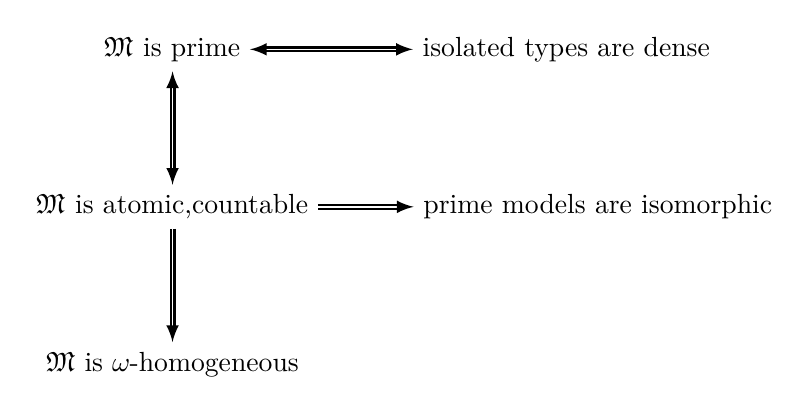
\begin{tikzpicture}
[a/.style={latex-latex,double,thick},
b/.style={-latex,thick,double}]
\node (1) {\(\fM\) is prime};
\node (2) [below of=1,yshift=-1cm] {\(\fM\) is atomic,countable};
\node (3) [below of=2,yshift=-1cm] {\(\fM\) is \(\omega\)-homogeneous};
\node (4) [right of=1,xshift=4cm] {isolated types are dense};
\node (5) [below of=4,yshift=-1cm,xshift=0.4cm] {prime models are isomorphic};
\draw[a] (1) -- (2);
\draw[a] (1) -- (4);
\draw[b] (2) -- (5);
\draw[b] (2) -- (3);
\end{tikzpicture}\end{center}


Let \(T\) be a countable complete theory with infinite models
\index{ prime model}
\index{atomic model}
\begin{definition}[]
Let \(T\) be a countable theory with infinite models, not necessarily complete
\begin{enumerate}
\item We call \(\fA_0\) a \textbf{prime model} of \(T\) if \(\fA_0\) can be elementarily embedded into all
models of \(T\)
\item A structure \(\fA\) is called \textbf{atomic} if all \(n\)-tuples \(\bara\) of elements of \(\fA\) are
atomic. This means that the types \(\tp(\bara)\) are isolated in \(S_n^{\fA}(\emptyset)=S_n(T)\)
\end{enumerate}
\end{definition}

Prime models need not exists. By Corollary \ref{cor4.2.7}, a tuple \(\bara\) is atomic iff it
satisfies a complete formula.

Since \(T\) has countable models, prime models must be countable and since non-isolated types
can be omitted in suitable models by Theorem \ref{thm4.1.2}, only isolated types can be realised
in prime models.

\begin{theorem}[]
\label{thm4.5.2}
A model of \(T\) is prime iff it is countable and atomic
\end{theorem}

\begin{proof}
As just noted, a prime model has to be countable and atomic.

Let \(\fM_0\) be a countable and atomic model of \(T\) and \(\fM\) any model of \(T\). We construct
an elementary embedding of \(\fM_0\) to \(\fM\) as a union of an ascending sequence of elementary
maps
\begin{equation*}
f:A\to B
\end{equation*}
between finite subsets \(A\) of \(M_0\) and \(B\) of \(M\). The empty map is elementary
since \(T\) is complete and \(\fM_0\equiv\fM\)

We show that \(f\) can be extended to any given \(A\cup\{a\}\). Let \(p(x)=\tp(a/A)\)
and \(f(p)=f(p(x))\). We show that \(f(p)\) has a realisation \(b\in M\)

Let \(\bara\) be a tuple which enumerates the elements of \(A\) and \(\varphi(x,\barx)\)
an \(L\)-formula which isolates the \(\tp(a\bara)\) since \(\fM_0\) is atomic. Then \(p(x)\) is
isolated by \(\varphi(x,\bara)\): clearly \(\varphi(x,\bara)\in\tp(a/\bara)\) and
if \(\rho(x,\bara)\in\tp(a/\bara)\) we have  \(\rho(x,y)\in\tp(a,\bara)\). This implies
that \(\fM_0\vDash\forall x(\varphi(x,\bara)\to\rho(x,\bara))\) and \(\fM\vDash\forall x(\varphi(x,f(\bara))\to\rho(x,f(\bara)))\). Thus \(f(p)\) is
isolated by \(\varphi(x,f(\bara))\) and since \(\varphi(x,f(\bara))\) can be realised in \(\fM\), so can
be \(f(p)\).
\wu{
Now we prove \(f(p)\) is indeed a type. If there are \(\varphi(x,\barx)\in\tp(b\barb)\setminus f(p)\).
Then \(\fM_0\not\vDash\varphi(a,\bara)\) and thus \(\neg\varphi(x,\barx)\in f(p)\subseteq\tp(b\barb)\), a contradiction.
}
\end{proof}

\begin{theorem}[]
\label{thm4.5.3}
All prime models of \(T\) are isomorphic
\end{theorem}

\begin{proof}
Let \(\fM_0\) and \(\fM_0'\) be two prime models. Since prime models are atomic, elementary maps
between finite subsets of \(\fM_0\) and \(\fM_0'\) can be extended to all finite extensions.
Since \(\fM_0\) and \(\fM_0'\) are countable, it follows as Lemma \ref{lemma4.3.3} that \(\fM_0\cong\fM_0'\);''
\end{proof}

\begin{corollary}[]
Prime models are \(\omega\)-homogeneous
\end{corollary}

\begin{proof}
Let \(\fM_0\) be prime and \(\bara\) any tuple of elements from \(M_0\). By Theorem
\ref{thm4.5.2}, \((\fM_0,\bara)\) is a prime model of its theory
\wu{
as it's still countable and atomic
}
. The claim follows now from Theorem \ref{thm4.5.3}
\end{proof}


\begin{definition}[]
The isolated types are \textbf{dense} in \(T\) if every consistent \(L\)-formulas \(\psi(x_1,\dots,x_n)\) belongs
to an isolated type \(p(x_1,\dots,x_n)\in S_n(T)\)
\end{definition}

\begin{theorem}[]
\label{thm4.5.7}
\(T\) has a prime model iff the isolated types are dense
\end{theorem}

\begin{proof}
Suppose \(T\) has a prime model \(\fM\) (so \(\fM\) is atomic by Theorem \ref{thm4.5.2}). Since
consistent formulas \(\psi(\barx)\) are realised in all models of \(T\), \(\psi(\barx)\) is realised
by an atomic tuple \(\bara\) and \(\psi(\barx)\) belongs to the isolated type \(\tp(\bara)\)

For the other direction notice that a structure \(\fM_0\) is atomic iff for all \(n\) the set
\begin{equation*}
\Sigma_n(x_1,\dots,x_n)=\{\neg\varphi(x_1,\dots,x_n)\mid\varphi(x_1,\dots,x_n)\text{ complete}\}
\end{equation*}
is not realised in \(\fM_0\).
\wu{
\(\bara\) is atomic iff it realise at least one complete formula.
}
Hence by Corollary \ref{cor4.1.3}, it's enough to show that the \(\Sigma_n\) are not isolated in \(T\).
This is the case iff for every consistent \(\psi(x_1,\dots,x_n)\) there is a complete
formula \(\varphi(x_1,\dots,x_n)\) with \(T\not\vDash\forall\barx(\psi(\barx)\to\neg\varphi(\barx))\).
\wu{
\(\Sigma_n\) is not isolated iff for every complete formula \(\theta\) there exists \(\gamma\in\Sigma_n\)
s.t. \(T\not\vDash\theta\to\gamma\). \(\gamma\) here is of the form \(\neg\varphi\) and we loose the condition of \(\theta\).
}
Since \(\varphi(\barx)\) is
complete, this is equivalent to \(T\vDash\forall\barx(\varphi(\barx)\to\psi(\barx))\). We conclude that \(\Sigma_n\) is not
isolated iff the isolated \(n\)-types are dense
\end{proof}



\begin{examplle}[]
Let \(T\) be the language having a unary predicate \(P_s\) for every finite
0-1-sequence \(s\in 2^{<\omega}\). The axioms of \(\Tree\) say that the \(P_s,s\in 2^{<\omega}\), form a
binary decomposition of the universe
\begin{itemize}
\item \(\forall x\;P_\emptyset(x)\)
\item \(\exists x\;P_s(x)\)
\item \(\forall x\;((P_{s0}(x)\vee P_{s1}(x))\leftrightarrow P_s(x))\)
\item \(\forall x\;\neg(P_{s0}(x)\wedge P_{s1}(x))\)
\end{itemize}


\(\Tree\) is complete and has quantifier elimination. There are no complete formulas and no
prime model
\end{examplle}


See Marker to see the full content
\begin{definition}[]
A family of formulas \(\varphi_s(\barx)\), \(s\in 2^{<\omega}\) is a \textbf{binary tree} if for all \(s\in 2^{<\omega}\) the
following holds
\begin{enumerate}
\item \(T\vDash\forall \barx\;((\varphi_{s0}(\barx)\vee\varphi_{s1}(\barx))\to\varphi_s(\barx))\)
\item \(T\vDash\forall\barx\;\neg(\varphi_{s0}(\barx)\wedge\varphi_{s1}(\barx))\)
\end{enumerate}
\end{definition}

\begin{theorem}[]
\label{thm4.5.9}
Let \(T\) be a complete theory
\begin{enumerate}
\item If \(T\) is small, it has no binary tree of consistent \(L\)-formulas. If \(T\) is countable,
the converse holds as well
\item If \(T\) has no binary tree of consistent \(L\)-formulas, the isolated types are dense
\end{enumerate}
\end{theorem}

\begin{proof}
\begin{enumerate}
\item Let \((\varphi_s(x_1,\dots,x_n))\) be a binary tree of consistent formulas. Then, for all \(\eta\in 2^\omega\),
the set
\begin{equation*}
\{\varphi_s(\barx)\mid s\subseteq\eta\}
\end{equation*}
is consistent and therefore is contained in some type \(p_{\eta}(\barx)\in S_n(T)\).
The \(p_\eta(\barx)\) are all different showing that \(T\) is not small.
\end{enumerate}
\end{proof}

\begin{exercise}
Countable theories without a binary tree of consistent formulas are small
\end{exercise}

\begin{proof}
If countable theory \(T\) is not small.
\end{proof}

\begin{exercise}
\label{ex4.5.2}
Show that isolated types being dense is equivalent to isolated types being (topologically) dense
in the Stone space \(S_n(T)\).
\end{exercise}

\begin{proof}
Let \(S=\{\text{the isolated types in }S_n(T)\}\). \(S\) is dense in \(S_n(T)\)
iff \(\barS=S_n(T)\). For any \(p\in S_n(T)\setminus S\), \(p\) is non-isolated. For any \(p\in[\phi]\), \(\phi\)
belongs to an isolated type \(q\). Thus \(q\in S_n(T)\cap S\). Hence \(\barS=S_n(T)\).
\end{proof}



\section{\texorpdfstring{\(\aleph_1\)}{ℵ₁}-categorical Theories}
\label{sec:org1651dd4}

\subsection{Indiscernibles}
\label{sec:orga118ad4}
\begin{definition}[]
Let \(I\) be a linear order and \(\fA\) an \(L\)-structure. A family \((a_i)_{i\in I}\) of elements
of \(A\) is called a \textbf{sequence of indiscernibles}  if for all \(L\)-formulas \(\varphi(x_1,\dots,x_n)\) and
all \(i_1<\dots<i_n\) and \(j_1<\dots<j_n\) from \(I\)
\begin{equation*}
\fA\vDash\varphi(a_{i_1},\dots,a_{i_n})\leftrightarrow\varphi(a_{j_1},\dots,a_{j_n})
\end{equation*}
\end{definition}

if two of the \(a_i\) are equal, all \(a_i\) are the same. Therefore it is often assumed that
the \(a_i\) are distinct

Sometimes sequences of indiscernibles are also called \textbf{order indiscernible} to distinguish them
from \textbf{totally indiscernible} sequences in which the ordering of the index set does not matter.

\begin{definition}[]
Let \(I\) be an infinite linear order and \(\cali=(a_i)_{i\in I}\) a sequence of \(k\)-tuples
in \(\fM\), \(A\subseteq M\). The \textbf{Ehrenfeucht-Mostowski type} \(\EM(\cali/A)\) of \(\cali\) over \(A\) is the set
of \(L(A)\)-formulas \(\varphi(x_1,\dots,x_n)\) with \(\fM\vDash\varphi(a_{i_1},\dots,a_{i_n})\) for all \(i_1<\dots<i_n\in I\), \(n<\omega\)
\end{definition}

\begin{lemma}[The Standard Lemma]
\label{lemma5.1.3}
Let \(I\) and \(J\) be two infinite linear orders and \(\cali=(a_i)_{i\in I}\) a sequence of elements
of a structure \(\fM\). Then there is structure \(\fN\equiv\fM\) with an indiscernible
sequences \((b_j)_{j\in J}\) realizing the Ehrenfeucht-Mostowski type \(\EM(\cali)\) of \(\cali\)
\end{lemma}

\wu{
We can also find a model \(\fN\succ\fM\)
}

\begin{corollary}[]
Assume that \(T\) has an infinite model. Then for any linear order \(I\), \(T\) has a model with
a sequence \((a_i)_{i\in I}\) of distinct indiscernibles
\end{corollary}

Let \([A]^n\) denote the set of all \(n\)-element subsets of \(A\)

\begin{theorem}[Ramsey]
Let \(A\) be infinite and \(n\in\omega\). Partition the set of \(n\)-elements subsets \([A]^n\) into
subsets \(C_1,\dots,C_k\). Then there is an infinite subset of \(A\) whose \(n\)-element subsets all
belong to the same subset \(C_i\)
\end{theorem}

\begin{proof}
Thinking of the partition as a colouring on \([A]^n\), we are looking for an infinite
subset \(B\) of \(A\) s.t. \([B]^n\) is monochromatic. We prove the theorem by induction
on \(n\). For \(n=1\), the statement is evident from the pigeonhole principle since there are
infinite elements and finite colors.

Assuming the theorem is true for \(n\), we now prove it for \(n+1\). Let \(a_0\in A\). Then any
colouring of \([A]^{n+1}\) induces a colouring of the \(n\)-element subsets of \(A'=A\setminus\{a_0\}\):
just colour \(x\in[A']^n\) by the colour of \(\{a_0\}\cup x\in[A]^{n+1}\). By the induction hypothesis,
there exists an infinite monochromatic subset \(B_1\) of \(A'\) in the induced colouring. Thus,
all the \((n+1)\)-element subsets of \(A\) consisting of \(a_0\) and \(n\) elements of \(B_1\)
have the same colour but \(\{a_0\}\cup B\) is not our desired set.

Now pick any \(a_1\in B_1\). By the same argument we obtain an infinite
subset \(B_2\subseteq B_1\) with the same properties. We thus construct an infinite
sequence \(A=B_0\supset B_1\supset B_2\supset\dots\) and elements \(a_i\in B_i\setminus B_{i+1}\) s.t.
the colour of each \((n+1)\)-element subset \(\{a_{i(0)},\dots,a_{i(n)}\}\) with \(i(0)<i(1)<\dots<i(n)\)
depends only on the value of \(i(0)\).
\begin{equation*}
a_0,a_1,a_2,\dots,a_n,\dots
\end{equation*}
Again by the pigeonhole principle there are infinitely
many values of \(i(0)\) for which this colour will be the same and we take \(\{a_{i(0)}\}\).
These \(a_{i(0)}\) then yields
the desired monochromatic set.
\end{proof}

\begin{proof}[Proof of Lemma \ref{ref:lemma5.1.3}]
Choose a set \(C\) of new constants with an ordering isomorphic to \(J\). Consider the theories
\begin{align*}
T'&=\{\varphi(\barc)\mid\varphi(\barx)\in\EM(\cali)\}\\
T''&=\{\varphi(\barc)\leftrightarrow\varphi(\bard)\mid\barc,\bard\in C\}
\end{align*}
Here the \(\varphi(\barx)\) are \(L\)-formulas and \(\barc,\bard\) tuples in increasing order. We have
to show that \(T\cup T'\cup T''\) is consistent. It is enough to show that
\begin{equation*}
T_{C_0,\Delta}=T\cup\{\varphi(\barc)\in T'\mid\barc\in C_0\}\cup\{\varphi(\barc)\leftrightarrow\varphi(\bard)\mid\varphi(\barx)\in\Delta,\barc,\bard\in C_0\}
\end{equation*}
is consistent for finite sets \(C_0\) and \(\Delta\). Note that \(\Diag_{\el}(\fM)\subseteq T\).
We can assume that the elements of \(\Delta\) are formulas
with free variables \(x_1,\dots,x_n\) and that all tuples \(\barc\) and \(\bard\) have the same
length

for notational simplicity we assume that all \(a_i\) are different. So we may
consider \(A=\{a_i\mid i\in I\}\) as an ordered set, which is the interpretation of \(C\). We define an
equivalence relation on \([A]^n\) by
\begin{equation*}
\bara\sim\barb\Longleftrightarrow\fM\vDash\varphi(\bara)\leftrightarrow\varphi(\barb)\text{ for all }\varphi(x_1,\dots,x_n)\in\Delta
\end{equation*}
where \(\bara,\barb\) are tuples in increasing order. Since this equivalence has at
most \(2^{\abs{\Delta}}\) many classes, by Ramsey's Theorem there is an infinite subset \(B\subseteq A\) with
all \(n\)-element subsets in the same equivalence class. We interpret the constants \(c\in C_0\)
by elements \(b_c\) in \(B\) ordered in the same way as the \(c\). Then \((\fM,b_c)_{c\in C_0}\) is
a model of \(T_{C_0,\Delta}\).
\end{proof}

\begin{lemma}[]
\label{lemma5.1.6}
Assume \(L\) is countable. If the \(L\)-structure \(\fM\) is generated by a well-ordered
sequence \((a_i)\) of indiscernibles, then \(\fM\) realises only countably many types over every
countable subset of \(M\)
\end{lemma}

\begin{proof}
\label{BIG Problem}: need more time to think

If \(A=\{a_i\mid i\in I\}\), then every element \(b\in M\) has the form \(b=t(\bara)\), where \(t\) is
an \(L\)-term and \(\bara\) is a tuple from \(A\) since \(\fM\) is generated by \((a_i)\)

Consider a countable subset \(S\) of \(M\). Write
\begin{equation*}
S=\{t_n^{\calm}(\bara^n)\mid n\in\omega\}
\end{equation*}
Let \(A_0=\{a_i\mid i\in I_0\}\) be the (countable) set of elements of \(A\) which occur in
the \(\bara^n\). Then every type \(\tp(b/S)\) is determined by \(\tp(b/A_0)\) since
every \(L(S)\)-formula
\begin{equation*}
\varphi(x,t_{n_1}^{\calm}(\bara^{n}),\dots)
\end{equation*}
can be replaced by the \(L(A_0)\)-formula \(\varphi(x,t_{n_1}(\bara^{n_1}),\dots)\)

\(\tp(b/A_0)=\tp(t(\bara)/A_0)=\{\varphi(\barx)\; \call_{A_0}\text{-formula}: \fM\vDash\varphi(t(\bara))\}\).

Now the type of \(b=t(\bara)\) over \(A_0\) depends only on \(t(\barx)\) (countably many
possibilities) and the type \(\tp(\bara/A_0)\) (really?). Write \(\bara=a_{\bari}\) for a tuple \(\bari\)
from \(I\). \uline{Since the \(a_i\) are indiscernible, the type depends only on}
\uline{the quantifier-free type \(\tp_{\qf}(\bari/I_0)\) in the structure \((I,<)\)} since it has
quantifier elimination. This type again depends on \(\tp_{\qf}(\bari)\) (finitely many
possibilities) and on the types  \(p(x)=\tp_{\qf}(i/I_0)\) of the elements \(i\) (Note the
quantifier elimination, then we only need to Booleanly combine these things to get \(\tp_{\qf}(\bari/I_0)\))
of \(\bari\). There are three kinds of such types:
\begin{enumerate}
\item \(i\) is bigger than all elements of \(I_0\)
\item \(i\) is an element \(i_0\) of \(I_0\)
\item For some \(i_0\in I_0\), \(i\) is smaller than \(i_0\) but bigger than all elements
of \(\{j\in I_0\mid j<i_0\}\)
\end{enumerate}


There is only one type in the first case, in the other case the type is determined by \(i_0\).
This results in countably many possibilities for each component of \(\bari\)
\end{proof}

\begin{definition}[]
Let \(L\) be a language. A \textbf{Skolem theory} \(\Skolem(L)\) is a theory in a bigger
language \(L_{\Skolem}\) with the following properties
\begin{enumerate}
\item \(\Skolem(L)\) has quantifier elimination
\item \(\Skolem(L)\) is universal
\item Every \(L\)-structure can be expanded to a model of \(\Skolem(L)\)
\item \(\abs{L_{\Skolem}}\le\max(\abs{L},\aleph_0)\)
\end{enumerate}
\end{definition}

\begin{theorem}[]
Every language \(L\) has a Skolem theory.
\end{theorem}

\begin{proof}
Nice \href{http://www-verimag.imag.fr/\~monin/EnseignementPublic/Misc/L2/INF242/Slides/cours09skolem\_En.pdf}{slide}. We have
\begin{enumerate}
\item \(\exists xP(x)\) is a consequence of \(P(a)\)
\item \(P(a)\) is not a consequence of \(\exists xP(x)\), but a model of \(\exists xP(x)\) \textbf{provides} a model
of \(P(a)\)
\end{enumerate}


Skolemization eliminates existential quantifiers and transforms a closed formula \(A\) to a formula \(B\) such that :
\begin{itemize}
\item \(A\) is a consequence of \(B\), \(B\vDash A\)
\item every model of A \textbf{provides} a model of B
\end{itemize}


Hence, \(A\) has a model if and only if \(B\) has a model : \emph{skolemization preserves the
existence of a model}, in other words \emph{it preserves satisfiability}.


We define an ascending sequence of languages
\begin{equation*}
L=L_0\subseteq L_1\subseteq L_2\subseteq\cdots
\end{equation*}
by introducing for every quantifier-free \(L_i\)-formula \(\varphi(x_1,\dots,x_n,y)\) a new \(n\)-place
\textbf{Skolem function}  \(f_\varphi\) (if \(n=0\), \(f_\varphi\) is a constant) and defining \(L_{i+1}\) as the
union of \(L_i\) and the set of these function symbols. The language \(L_{\Skolem}\) is the union
of all \(L_i\). We now define the Skolem theory as
\begin{equation*}
\Skolem=\{\forall\barx(\exists y\varphi(\barx,y)\to\varphi(\barx,f_\varphi(\barx)))\mid\varphi(\barx,y)\text{ q.f. $L_{\Skolem}$-formula}\}
\end{equation*}
\end{proof}

\begin{corollary}[]
\label{cor5.1.9}
Let \(T\) be a countable theory with an infinite model and let \(\kappa\) be an infinite cardinal.
Then \(T\) has a model of cardinality \(\kappa\) which realises only countably many types over every
countable subset.
\end{corollary}

\begin{proof}
Consider the theory \(T^*=T\cup\Skolem(L)\). Then \(T^*\) is countable, has an infinite model and
quantifier elimination

\textbf{Claim}. \(T^*\) is equivalent to a universal theory

\emph{Proof}. Modulo \(\Skolem(L)\) every axiom \(\varphi\) of \(T\) is equivalent to a
quantifier-free \(L_\Skolem\)-sentence \(\varphi^*\). Therefore \(T^*\) is equivalent to the universal
theory

Let \(I\) be a well-ordering of cardinality \(\kappa\) and \(\fN^*\) a model of \(T^*\) with
indiscernibles \((a_i)_{i\in I}\) (Existence by the Standard Lemma \ref{lemma5.1.3}). The claim
implies that the substructure \(\fM^*\) generated by
the \(a_i\) is a model of \(T^*\) and \(\fM^*\) has cardinality \(\kappa\) (As we can't control the size of
an elementary extension and Corollary \ref{cor3.1.5}). Since \(T^*\) has quantifier
elimination, \(\fM^*\) is an elementary substructure of \(\fN^*\) and \((a_i)\) is indiscernible
in \(\fM^*\). By Lemma \ref{lemma5.1.6}, there are only countably many types over every countable
set realised in \(\fM^*\). The same is then true for the reduct \(\fM=\restr{\fM^*}{L}\)
\end{proof}

\begin{exercise}
\label{ex5.1.1}
A sequence of elements in \((\Q,<)\) is indiscernible iff it is either constant, strictly
increasing or strictly decreasing
\end{exercise}

\begin{proof}
For any formula \(\varphi(x_1,x_2,\dots,x_n)\),
\begin{equation*}
\Q\vDash\varphi(x_1,x_2,\dots,x_n)\leftrightarrow
\end{equation*}
\end{proof}

\subsection{\texorpdfstring{\(\omega\)}{ω}-stable theories}
\label{sec:orgb72102a}
In this section we fix a complete theory \(T\) with infinite models

Our goal is theorem \ref{thm5.2.11}
\begin{theorem}[]
A countable theory \(T\) is \(\kappa\)-categorical iff all models of cardinality \(\kappa\) are saturated
\end{theorem}

\begin{center}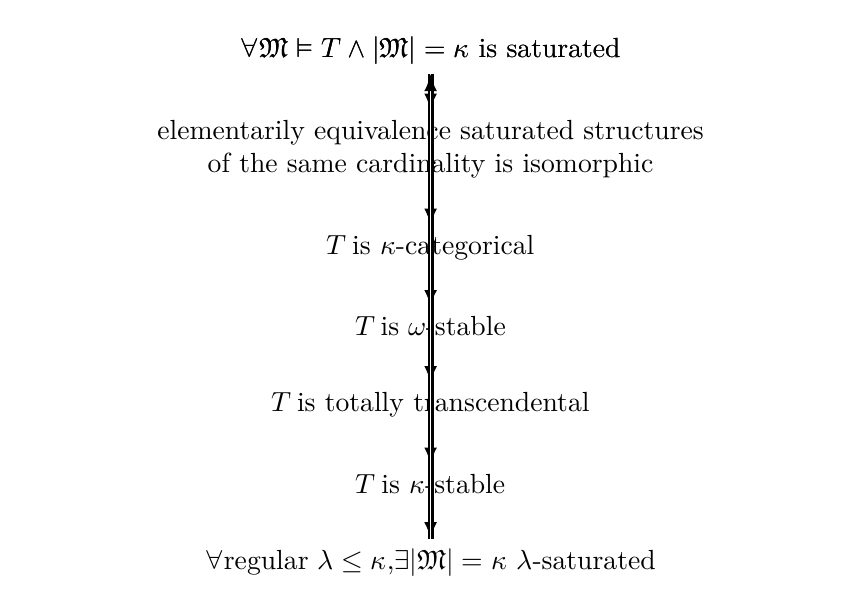
\begin{tikzpicture}
[a/.style={latex-latex,double,thick},
b/.style={-latex,thick,double}]
\node (2) {\(\forall\fM\vDash T\wedge\abs{\fM}=\kappa\) is saturated};
\node (7) [below of=2,text width=10cm,align=center,yshift=-0.25cm]{elementarily equivalence saturated structures\\ of the same cardinality is isomorphic};
\node (1) [below of=7,yshift=-0.25cm]{\(T\) is \(\kappa\)-categorical};
\node (3) [below of=1] {\(T\) is \(\omega\)-stable};
\node (4) [below of=3] {\(T\) is totally transcendental};
\node (5) [below of=4] {\(T\) is \(\kappa\)-stable};
\node (6) [below of=5] {\(\forall\)regular \(\lambda\le\kappa\),\(\exists\abs{\fM}=\kappa\) \(\lambda\)-saturated};
\node (8) {\(\forall\fM\vDash T\wedge\abs{\fM}=\kappa\) is saturated};
\draw[b] (2) -- (7);
\draw[b] (7) -- (1);
\draw[b] (1) -- (3);
\draw[b] (3) -- (4);
\draw[b] (4) -- (5);
\draw[b] (5) -- (6);
\draw[b] (6) -- (8);
\end{tikzpicture}\end{center}


In the previous section we saw that we may add indiscernible elements to a model without
changing the number of realised types. We will now use this to show that \(\aleph_1\)-categorical
theories a small number of types, i.e., they are \(\omega\)-stable. Conversely, with few types it is
easier to be saturated and since saturated structures are unique we find the connection to
categorical theories.

\begin{definition}[]
Let \(\kappa\) be an infinite cardinal. We say \(T\) is \textbf{\(\kappa\)-stable} if in each model of \(T\), over
every set of parameters of size at most \(\kappa\), and for each \(n\), there are at most \(\kappa\)
many \(n\)-types, i.e.,
\begin{equation*}
\abs{A}\le\kappa\Rightarrow\abs{S_n(A)}\le\kappa
\end{equation*}
\end{definition}

Note that if \(T\) is \(\kappa\)-stable, then - up to logical equivalence - we have \(\abs{T}\le\kappa\)
(Exercise \ref{ex5.2.6})

\begin{lemma}[]
\label{lemma5.2.2}
\(T\) is \(\kappa\)-stable iff \(T\) is \(\kappa\)-stable for 1-types, i.e.,
\begin{equation*}
 \abs{A}\le\kappa\Rightarrow\abs{S(A)}\le\kappa
\end{equation*}
\end{lemma}

\begin{proof}
Assume that \(T\) is \(\kappa\)-stable for 1-types. We show that \(T\) is \(\kappa\)-stable for \(n\)-types by
induction on \(n\). Let \(A\) be a subset of the model \(\fM\) and \(\abs{A}\le\kappa\). We may assume
that all types over \(A\) are realised in \(\fM\) (otherwise we take some elementary extensions by
Corollary \ref{cor2.2.9}). Consider the restriction map \(\pi:S_n(A)\to S_1(A)\). By assumption the
image \(S_1(A)\) has cardinality at most \(\kappa\).
Every \(p\in S_1(A)\) has the form \(\tp(a/A)\) for some \(a\in M\) since all types over \(A\) are
realized in \(\fM\). By Exercise \ref{ex4.2.5}, the fibre \(\pi^{-1}(p)\) is in bijection
with \(S_{n-1}(aA)\) and so has cardinality at most \(\kappa\) by induction. This shows \(\abs{S_n(A)}\le\kappa\cdot\kappa=\kappa\).
\end{proof}

\begin{examplle}[Algebraically closed fields]
The theories \(\ACF_p\) for \(p\) a prime or 0 are \(\kappa\)-stable for all \(\kappa\)
\end{examplle}

Note that by Theorem \ref{thm5.2.6} below it would suffice to prove that the theories \(\ACF_p\)
are \(\omega\)-stable

\begin{proof}
\label{Problem1}
Let \(K\) be a subfield of an algebraically closed field. By quantifier elimination, the type of
\uline{an element \(a\) over \(K\) is determined by the isomorphism type of the extension \(K[a]/K\)}.
If \(a\) is transcendental over \(K\), \(K[a]\) is isomorphic to the polynomial ring \(K[X]\).
If \(a\) is algebraic with minimal polynomial \(f\in K[X]\), then \(K[a]\) is isomorphic
to \(K[X]/(f)\). \uline{So there is one more 1-type over \(K\) than there are irreducible polynomials}
\end{proof}

That \(\ACF_p\) is \(\kappa\)-stable for \(n\)-types has a direct algebraic proof: the isomorphism type
of \(K[a_1,\dots,a_n]/K\) is determined by the vanishing ideal \(P\) of \(a_1,\dots,a_n\). By :((((

\begin{theorem}[]
\label{thm5.2.4}
A countable theory \(T\) which is categorical in an uncountable cardinal \(\kappa\) is \(\omega\)-stable
\end{theorem}

\begin{proof}
Let \(\fN\) be a model and \(A\subseteq N\) countable with \(S(A)\) uncountable. Let \((b_i)_{i\in I}\) be a
sequence of \(\aleph_1\) many elements with pairwise distinct types over \(A\). (Note that we can
assume that all types over \(A\) are realised in \(\fN\)) We choose first an elementary
substructure \(\fM_0\) of cardinality \(\aleph_1\) which contains \(A\) and all \(b_i\). Then we choose an
elementary extension \(\fM\) of \(\fM_0\). The model \(\fM\) is of cardinality \(\kappa\) and realises
uncountably many types over the countable set \(A\). By Corollary \ref{cor5.1.9}, \(T\) has another
model where this is not the case. So \(T\) cannot be \(\kappa\)-categorical
\end{proof}

\index{totally transcendental}
\begin{definition}[]
A theory \(T\) is \textbf{totally transcendental} if it has no model \(\fM\) with a binary tree of
consistent \(L(M)\)-formulas
\end{definition}

\begin{theorem}[]
\label{thm5.2.6}
\begin{enumerate}
\item \(\omega\)-stable theories are totally transcendental
\item Totally transcendental theories are \(\kappa\)-stable for all \(\kappa\ge\abs{T}\)
\end{enumerate}
\end{theorem}

It follows that a countable theory \(T\) is \(\omega\)-stable iff it is totally transcendental

\begin{proof}
\begin{enumerate}
\item Let \(\fM\) be a model with a binary tree of consistent \(L(M)\)-formulas with free variables
among \(x_1,\dots,x_n\). The set \(A\) of parameters which occur in the tree's formulas is
countable but \(S_n(A)\) has cardinality \(2^{\aleph_0}\)
\item Assume that there are there are more than \(\kappa\) many \(n\)-types over some set \(A\) of
cardinality \(\kappa\). Let us call an \(L(A)\)-formula \textbf{big} if it belongs to more than \(\kappa\) many types
over \(A\) (\(\abs{[\phi]}>\kappa\)) and \textbf{thin} otherwise. By assumption the true formula is big. If we
can show that each big formula decomposes into two big formulas, we can construct a binary
tree of big formulas, which finishes the proof.

So assume that \(\varphi\) is big. Since each thin formula belongs to at most \(\kappa\) types and since there
are at most \(\kappa\) formulas, there are at most \(\kappa\) types which contain thin formulas. Therefore
\(\varphi\) belongs to two distinct types \(p\) and \(q\) which contain only big formulas. If we
separate \(p\) and \(q\) by \(\psi\in p\) and \(\neg\psi\in q\), we decompose \(\varphi\) into the big
formulas \(\varphi\wedge\psi\) and \(\varphi\wedge\neg\psi\).
\end{enumerate}
\end{proof}

The proof and Lemma \ref{lemma5.2.2} show that \(T\) is totally transcendental iff there is no
binary tree of consistent formulas in \textbf{one} free variables

The general case follows from Exercise \ref{ex5.2.5}

\begin{definition}[]
Let \(\kappa\) be an infinite cardinal. An \(L\)-structure \(\fA\) is \textbf{\(\kappa\)-saturated} if in \(\fA\) all
types over sets of cardinality less than \(\kappa\) are realised. An infinite structure \(\fA\) is \textbf{saturated}
if it is \(\abs{\fA}\)-saturated
\end{definition}

Lemma \ref{lemma4.3.3} generalises to sets

\begin{lemma}[]
\label{lemma5.2.8}
Elementarily equivalent saturated structures of the same cardinality are isomorphic
\end{lemma}

\begin{proof}
Let \(\fA\) and \(\fB\) be elementary equivalent saturated structures each of cardinality \(\kappa\). We
choose enumerations \((a_\alpha)_{\alpha<\kappa}\) and \((b_\alpha)_{\alpha<\kappa}\) of \(A\) and \(B\) and construct an
increasing sequence of elementary maps \(f_\alpha:A_\alpha\to B_\alpha\). Assume that the \(f_\beta\) are constructed
for all \(\beta<\alpha\). The union of the \(f_\beta\) is an elementary map \(f_\alpha^*:A_\alpha^*\to B_\alpha^*\). The
construction will imply that \(A_\alpha^*\) and \(B_\alpha^*\) have cardinality at most \(\abs{\alpha}\), which
is smaller than \(\kappa\)

We write \(\alpha=\lambda+n\), and distinguish two cases

\(n=2i\): In this case, we consider \(p(x)=\tp(a_{\lambda+i}/A_\alpha^*)\). Realise \(f_\alpha^*(p)\) by \(b\in B\)
and define
\begin{equation*}
f_\alpha=f_\alpha^*\cup\{\la a_{\lambda+i},b\ra\}
\end{equation*}

\(n=2i+1\): Similarly, we find an extension
\begin{equation*}
f_\alpha=f_\alpha^*\cup\{\la a,b_{\lambda+i}\ra\}
\end{equation*}
Thus \(\bigcup_{\alpha<\kappa}f_\alpha\) is the desired isomorphism
\end{proof}

\begin{lemma}[]
Let \(S_0\subseteq S_1\subseteq\cdots\subseteq S_\alpha\subseteq\cdots\) be an increasing chain of sets indexed by \(\alpha<\kappa\) for some regular
cardinal \(\kappa\). If \(A\subseteq\bigcup_{\alpha<\kappa}S_\alpha\) and \(\abs{A}<\kappa\), then \(A\subseteq S_\alpha\) for some \(\alpha<\kappa\)
\end{lemma}

\begin{proof}
Define \(f:A\to\kappa\) by \(f(x)=\min\{\alpha:x\in S_\alpha\}\). Then \(\abs{f(A)}\le\abs{A}<\kappa\),
so \(\alpha:=\sup f(A)<\kappa\). For any \(x\in A\), we have \(f(x)\le\alpha\), and so \(x\in S_{f(x)}\subseteq S_\alpha\) and
thus \(A\subseteq S_\alpha\)
\end{proof}

\begin{lemma}[]
\label{lemma5.2.9}
If \(T\) is \(\kappa\)-stable, then for all regular \(\lambda\le\kappa\), there is a model of cardinality \(\kappa\) which is \(\lambda\)-saturated
\end{lemma}

\begin{proof}
By Exercise \ref{ex5.2.6} we may assume that \(\abs{T}\le\kappa\).  Consider a model \(\fM\) of cardinality
\(\kappa\). Since \(S(M_\alpha)\) has cardinality \(\kappa\), Corollary \ref{cor2.2.9} and the Löwenheim–Skolem theorem
give an elementary extension of cardinality \(\kappa\) in which all types over \(\fM\) are realised. So can
construct a continuous elementary chain
\begin{equation*}
\fM_0\prec\fM_1\prec\dots\prec\fM_\alpha\prec\cdots(\alpha<\lambda)
\end{equation*}
of models of \(T\) with cardinality \(\kappa\) s.t. all \(p\in S(M_\alpha)\) are realised in \(\fM_{\alpha+1}\).
Then \(\fM\) is \(\lambda\)-saturated. In fact, if \(\abs{A}<\lambda\) and if \(a\in A\) is contained in \(M_{\alpha(a)}\)
then \(\Lambda=\bigcup_{a\in A}\alpha(a)\) is an initial segment of \(\lambda\) of smaller cardinality than \(\lambda\).
\wu{
We can find since \(\kappa\) is regular iff \(\cf(\kappa)=\kappa\) iff \(\forall\alpha<\kappa\), \(\bigcup_{\beta<\alpha}M_\alpha\subsetneq M\). Thus
there is \(\gamma<\kappa\) s.t. \(\bigcup_{\beta<\alpha}S_\alpha\)
}
So \(\Lambda\) has an upper bound \(\mu<\lambda\). It follows that \(A\subseteq\fM_\mu\) and all types over \(A\) are realised
in \(\fM_{\mu+1}\)
\end{proof}

\begin{remark}
\label{re5.2.10}
If \(T\) is \(\kappa\)-stable for a regular cardinal \(\kappa\), the previous lemma yields a saturated model of
cardinality \(\kappa\).
\end{remark}

\begin{theorem}[]
\label{thm5.2.11}
A countable theory \(T\) is \(\kappa\)-categorical iff all models of cardinality \(\kappa\) are saturated
\end{theorem}

\begin{proof}
If all models of cardinality \(\kappa\) are saturated, it follows from Lemma \ref{lemma5.2.8} that \(T\) is
\(\kappa\)-categorical

Assume, for the converse that \(T\) is \(\kappa\)-categorical. For \(\kappa=\aleph_0\) the theorem follows from
Theorem \ref{thm4.3.1}. So we may assume that \(\kappa\) is uncountable. Then \(T\) is totally
transcendental by Theorem \ref{thm5.2.4} and \ref{thm5.2.6} and therefore \(\kappa\)-stable by Theorem
\ref{thm5.2.6}.

By Lemma \ref{lemma5.2.9}, \uline{all models of \(T\) of cardinality \(\kappa\) are \(\mu^+\)-saturated for}
\uline{all \(\mu<\kappa\). i.e., \(\kappa\)-saturated}
\end{proof}



\begin{exercise}
\label{ex5.2.2}
Show that the theory of an equivalence relation with two infinite classes has quantifier
elimination and is \(\omega\)-stable. Is it \(\aleph_1\)-categorical?
\end{exercise}


\begin{exercise}
\label{ex5.2.5}
If \(T\) is an \(L\)-theory and \(K\) is a sublanguage of \(L\), the \textbf{reduct} \(T\restriction K\) is
the set of all \(K\)-sentences which follow from \(T\). Show that \(T\) is totally transcendental
iff \(T\restriction K\) is \(\omega\)-stable for all at most countable \(K\subseteq L\)
\end{exercise}

\begin{proof}

\end{proof}

\begin{exercise}
\label{ex5.2.6}
If \(T\) is \(\kappa\)-stable, then \emph{essentially} (i.e., up to logical equivalence) \(\abs{T}\le\kappa\)
\end{exercise}

\begin{proof}
First for any \(\varphi,\psi\in T\), define \(\varphi\sim\psi\) iff \(T\vDash\varphi\leftrightarrow\psi\). If \(\abs{T/\sim}>\kappa\).

If \(T\not\vDash\varphi\leftrightarrow\psi\), then \(T\vDash(\varphi\wedge\neg\psi)\vee(\neg\varphi\wedge\psi)\). Thus for any non-equivalent \(\varphi\) and \(\psi\), they belong to
different types. Thus \(S_n(T)>\kappa\).

If \(T\) is \(\kappa\)-stable, then \(\abs{S_n(\emptyset)}\le\kappa\). Choose for any two \(n\)-types over the empty set
a separating formula \(\varphi\). Then any formula is logically equivalent to a finite Boolean combination
of these \(\kappa\)-many formulas.
\end{proof}

\subsection{Prime extensions}
\label{sec:orge32c284}
For any model \(\fM\vDash T\) and any \(A\subseteq\fM\)

  \begin{center}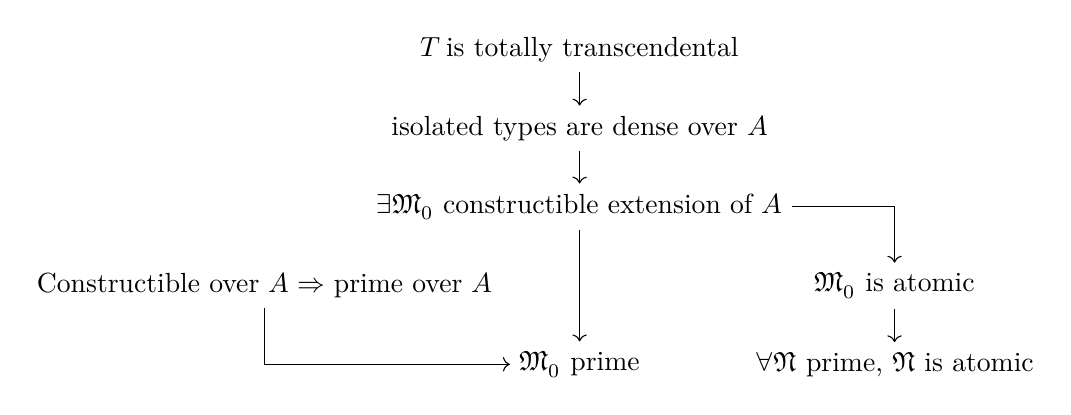
\begin{tikzpicture}
\node (1)  {\(T\) is totally transcendental};
\node (2) [below of=1] {isolated types are dense over \(A\)};
\node (3) [below of=2] {\(\exists\fM_0\) constructible extension of \(A\)};
\node (4) [left of=3,xshift=-3cm,yshift=-1cm] {Constructible over \(A\Rightarrow\) prime over \(A\)};
\node (5) [below of=3,yshift=-1cm] {\(\fM_0\) prime};
\node (6) [right of=3,xshift=3cm,yshift=-1cm] {\(\fM_0\) is atomic};
\node (7) [below of=6] {\(\forall\fN\) prime, \(\fN\) is atomic};
\draw[->] (1) -- (2);
\draw[->] (2) -- (3);
\draw[->] (3) -- (5);
\draw[->] (4) |- (5);
\draw[->] (3) -| (6);
\draw[->] (6) -- (7);
  \end{tikzpicture}\end{center}


\begin{definition}[]
Let \(\fM\) be a model of \(T\) and \(A\subseteq M\).
\begin{enumerate}
\item \(\fM\) is a \textbf{prime extension} of \(A\) (or \textbf{prime over} \(A\)) if every elementary map \(A\to\fN\)
extends to an elementary map \(\fM\to\fN\)
\begin{center}\begin{tikzcd}
\fM\ar[r]&\fN\\
A\ar[u,"id_A"]\ar[ur]
\end{tikzcd}\end{center}
\item \(B\subseteq M\) is \textbf{constructible} over \(A\) if \(B\) has an enumeration
\begin{equation*}
B=\{b_\alpha\mid\alpha<\lambda\}
\end{equation*}
where each \(b_\alpha\) is atomic over \(A\cup B_\alpha\) (\(\tp(b_\alpha/A\cup B_\alpha)\) is isolated), with \(B_\alpha=\{b_\mu\mid \mu<\alpha\}\)
\end{enumerate}
\end{definition}

So \(\fM\) is a prime extension of \(A\) iff \(\fM_A\) is a prime model of \(\Th(\fM_A)\)

\begin{lemma}[]
\label{lemma5.3.2}
If a model \(M\) is constructible over \(A\), then \(\fM\) is prime over \(A\)
\end{lemma}

\begin{proof}
Let \((m_\alpha)_{\alpha<\lambda}\) an enumeration of \(M\), s.t. each \(m_\alpha\) is atomic over \(A\cup M_\alpha\).
Let \(f:A\to\fN\) be an elementary map. We define inductively an increasing sequence of elementary
maps \(f_\alpha:A\cup M_{\alpha+1}\to\fN\) with \(f_0=f\). Assume that \(f_\beta\) is defined for all \(\beta<\alpha\). The
union of these \(f_\beta\) is an elementary map \(f_\alpha':A\cup M_\alpha\to\fN\). Since \(p(x)=\tp(a_\alpha/A\cup M_\alpha)\) is
isolated, \(f_\alpha'(p)\in S(f_\alpha'(A\cup M_\alpha))\) is also isolated and has a realisation \(b\) in \(\fN\). We
set \(f_\alpha=f_\alpha'\cup\{\la a_\alpha,b\ra\}\)

Finally, the union of all \(f_\alpha\) (\(\alpha<\lambda\)) is an elementary embedding \(\fM\to\fN\).
\end{proof}

\begin{theorem}[]
\label{thm5.3.3}
If \(T\) is totally transcendental, every subset of a model of \(T\) has a constructible prime extension
\end{theorem}

\wu{
Marker's Theorem 4.2.11
}

\begin{lemma}[]
\label{lemma5.3.4}
If \(T\) is totally transcendental, the isolated types are dense over every subset of any model
\end{lemma}

\begin{proof}
Consider a subset \(A\) of a model \(\fM\). Then \(\Th(\fM_A)\supset T\) has no binary tree of consistent
formulas. By Theorem \ref{thm4.5.9}, the isolated types in \(\Th(\fM_A)\) are dense
\end{proof}

\begin{proof}[Proof of Theorem \ref{thm5.3.3}]
By Lemma \ref{lemma5.3.2} it suffices to construct an elementary substructure \(\fM_0\prec\fM\) which
contains \(A\) and is constructible over \(A\). An application of Zorn's Lemma gives us a
maximal construction \((a_\alpha)_{\alpha<\lambda}\), which cannot be prolonged by an element \(a_\lambda\in M\setminus A_\lambda\).
\wu{
We need to show first that we can find \(a\) s.t. \(a\) is atomic over \(A\). But as the
isolated types are dense over \(A\), pick an \(L(A)\)-formula \(\varphi\) s.t. \(\fM\vDash\varphi(a)\). Then \(a\) is
atomic over \(A\).
}
Clearly \(A\) is contained in \(A_\lambda\). We show that \(A_\lambda\) is the universe of an elementary
substructure \(\fM_0\) using Tarski's Test. So assume that \(\varphi(x)\) is an \(L(A_\lambda)\)-formula
and \(\fM\vDash\exists x\varphi(x)\). Since isolated types over \(A_\lambda\) are dense by Lemma \ref{lemma5.3.4}, there is
an isolated \(p(x)\in S(A_\lambda)\) containing \(\varphi(x)\). Let \(b\) be a realisation of \(p(x)\)
in \(\fM\). We can prolong our construction by \(a_\lambda=b\); thus \(b\in A_\lambda\) by maximality
and \(\varphi(x)\) is realised in \(A_\lambda\).
\end{proof}

\begin{lemma}[]
\label{lemma5.3.5}
Let \(a\) and \(b\) be two finite tuples of elements of a structure \(\fM\). Then \(\tp(ab)\) is
atomic iff \(\tp(a/b)\) and \(\tp(b)\) are atomic
\end{lemma}

\begin{proof}
If \(\varphi(x,y)\) isolates \(\tp(a,b)\). As in the proof of Theorem \ref{thm4.5.2}, \(\varphi(x,b)\)
isolates \(\tp(a/b)\) and we claim that \(\exists x\varphi(x,y)\) isolates \(p(y)=\tp(b)\): we
have \(\exists x\varphi(x,y)\in p(y)\) and if \(\sigma(y)\in p(y)\), then
\begin{equation*}
\fM\vDash\forall x,y(\varphi(x,y)\to\sigma(y))
\end{equation*}
Hence \(\fM\vDash\forall y(\exists x\varphi(x,y)\to\sigma(y))\).

Now conversely, assume that \(\rho(x,b)\) isolates \(\tp(a/b)\) and that \(\sigma(y)\)
isolates \(p(y)=\tp(b)\). Then \(\rho(x,y)\wedge\sigma(y)\) isolates. Firstly, \(\rho(x,y)\wedge\sigma(y)\in\tp(a,b)\).
If \(\varphi(x,y)\in\tp(a,b)\), then \(\varphi(x,b)\in\tp(a/b)\) and
\begin{equation*}
\fM\vDash\forall x(\rho(x,b)\to\varphi(x,b))
\end{equation*}
Hence
\begin{equation*}
\forall x(\rho(x,y)\to\varphi(x,y))\in p(y)
\end{equation*}
and it follows that
\begin{equation*}
\fM\vDash\forall y(\sigma(y)\to\forall x(\rho(x,y)\to\varphi(x,y)))
\end{equation*}
Thus \(\fM\vDash\forall x,y(\rho(x,y)\wedge\sigma(y)\to\varphi(x,y))\)
\end{proof}

\begin{corollary}[]
Constructible extensions are atomic
\end{corollary}

\begin{proof}
Let \(\fM_0\) be a constructible extension of \(A\) and let \(\bara\) be a tuple from \(M_0\). We
have to show that \(\bara\) is atomic over \(A\). We can clearly assume that the elements
of \(\bara\) are pairwise distinct and do not belong to \(A\). We can also permute the elements
of \(\bara\) so that
\begin{equation*}
\bara=a_\alpha\barb
\end{equation*}
for some tuple \(\barb\in A_\alpha\). Let \(\varphi(x,\barc)\) be an \(L(A_\alpha)\)-formula which is complete
over \(A_\alpha\) and satisfied by \(a_\alpha\)
\(a_\alpha\) is also atomic over \(A\cup\{\barb\barc\}\). Using induction, we know
that \(\barb\barc\) is atomic over \(A\).
\wu{
Note that \(\barb\barc\in A_\alpha\), then we find a smaller ordinal. This process will end as there is
no infinite decreasing sequence.
}
By Lemma \ref{lemma5.3.5} applied
to \((\fM_0)_A\), \(a_\alpha\barb\barc\) is atomic over \(A\), which implies that \(\bara=a_\alpha\barb\) is
atomic over \(A\).
\end{proof}

\begin{corollary}[]
\label{cor5.3.7}
If \(T\) is totally transcendental, prime extensions are atomic
\end{corollary}

\begin{proof}
Let \(\fM\) be a model of \(T\) and \(A\subseteq M\).  Since \(A\) has at least one constructible
extension \(\fM_0\) and since all prime extensions of \(A\) are contained in \(\fM_0\) (isomorphic
over \(A\) to elementary substructure of \(\fM_0\)), all prime extensions are atomic
\end{proof}

A structure \(\fM\) is called a \textbf{minimal} extension of the subset \(A\) if \(M\) has no proper
elementary substructure which contains \(A\)

\begin{lemma}[]
\label{lemma5.3.8}
Let \(\fM\) be a model of \(T\) and \(A\subseteq M\). If \(A\) has a prime extension and a minimal
extension, they are isomorphic over \(A\), i.e., there is an isomorphism fixing \(A\) elementwise
\end{lemma}

\begin{proof}
A prime extension embeds elementarily in the minimal extension. This embedding must be
surjective by minimality
\end{proof}

\begin{exercise}
\label{ex5.3.2}
For every countable \(T\) the following are equivalent
\begin{enumerate}
\item Every parameter set has a prime extension (We say that \(T\) \emph{has prime extensions})
\item Over every countable parameter set the isolated types are dense
\item Over every parameter set the isolated types are dense
\end{enumerate}
\end{exercise}

\begin{proof}
\(3\to 2\to 1\) is from the text.

\(1\to 3\) from Theorem \ref{thm4.5.7}
\end{proof}
\subsection{Lachlan's Theorem}
\label{sec:org9abf7ac}
\begin{theorem}[Lachlan]
\label{thm5.4.1}
Let \(T\) be totally transcendental and \(\fM\) an uncountable model of \(T\). Then \(\fM\) has
arbitrary large elementary extensions which omit every countable set of \(L(M)\)-formulas that
is omitted in \(\fM\).
\end{theorem}

\begin{proof}
We call an \(L(M)\)-formula \textbf{large} if its realisation set \(\varphi(\fM)\) is uncountable. Since there is
no infinite binary tree of large formulas, there exists a \textbf{minimal} large formula
\(\varphi_0(x)\) in the sense that for every \(L(M)\)-formula \(\psi(x)\) either \(\varphi_0(x)\wedge\psi(x)\)
or \(\varphi_0(x)\wedge\neg\psi(x)\) is at most countable. Now it's easy to see that
\begin{equation*}
p(x)=\{\psi(x)\mid\varphi_0(x)\wedge\psi(x)\text{ large}\}
\end{equation*}
is a type in \(S(M)\).
\wu{
For any formula \(\psi\), if \(\varphi(\fM)=(\varphi(\fM)\wedge\psi(\fM))\cup(\varphi(\fM)\wedge\neg\psi(\fM))\). So exactly one of it belongs to \(p(x)\).
}

Clearly \(p(x)\) contains no formula of the form \(x\dot{=}a\) for \(a\in M\), so \(p(x)\) is not
realised in \(M\). On the other hand, every countable subset \(\Pi(x)\subseteq p(x)\) is realised
in \(\fM\): since \(\varphi_0(\fM)\setminus\psi(\fM)=\varphi_0(\fM)\wedge\neg\psi(\fM)\) is at most countable for every \(\psi(x)\in\Pi(x)\), the
elements of \(\varphi_0(\fM)\) which do not belong to the union of these sets realised \(\Pi(x)\).

Let \(a\) be a realisation of \(p(x)\) in a (proper) elementary extension \(\fN\). By Theorem
\ref{thm5.3.3}, we can assume that \(\fN\) is atomic over \(\fM\cup\{a\}\).

Fix \(b\in N\). We have to show that every countable subset \(\Sigma(y)\subset\tp(b/M)\) is realised
in \(M\).
\wu{
If the countable set is omitted in \(\fM\), then it is omitted in \(\fN\).
}

Let \(\chi(x,y)\) be an \(L(M)\)-formula s.t. \(\chi(a,y)\) isolates \(q(y)=\tp(b/M\cup\{a\})\). If \(b\)
realised an \(L(M)\)-formula \(\sigma(y)\), we have \(\fN\vDash\forall y(\chi(a,y)\to\sigma(y))\). Hence the formula
\begin{equation*}
\sigma^*(x)=\forall y(\chi(x,y)\to\sigma(y))
\end{equation*}
belongs to \(p(x)\)
\wu{
\(p(x)=\tp^{\fN}(a/M)\).
}
Note that \(\exists y\chi(x,y)\) belongs also to \(p(x)\).

Choose an element \(a'\in M\) which satisfies
\begin{equation*}
\{\sigma^*(x)\mid\sigma\in\Sigma\}\cup\{\exists y\chi(x,y)\}
\end{equation*}
and choose \(b'\in M\) with \(\fM\vDash\chi(a',b')\). Since \(\fM\vDash\sigma^*(a')\), \(\fM\vDash\sigma(b')\). So \(b'\)
realises \(\Sigma(y)\).

We have shown that \(\fM\) has a proper elementary extension which realises no new countable set
of \(L(M)\)-formulas. By iteration we obtain arbitrarily long chains of elementary extensions
with the same property
\end{proof}

\begin{corollary}[]
\label{cor5.4.2}
A countable theory which is \(\kappa\)-categorical for some uncountable \(\kappa\), is \(\aleph_1\)-categorical
\end{corollary}

\begin{proof}
Let \(T\) be \(\kappa\)-categorical and assume that \(T\) is not \(\aleph_1\)-categorical. Then \(T\) has a
model \(\fM\) of cardinality \(\aleph_1\) which is not saturated by Theorem \ref{thm5.2.11}.
\begin{center}\begin{tikzcd}
\fM\ar[r,"\not\cong"]\ar[d,"\prec"']&\fN\ar[d,"\prec"]\\
\fM'\ar[r,"\cong"']&\fN'
\end{tikzcd}\end{center}
\wu{
For any sentence \(\phi\), \(\fM\vDash\phi\Rightarrow\fM'\vDash\phi\Rightarrow\fN'\vDash\phi\Rightarrow\fN\vDash\phi\). Thus \(\fM\equiv\fN\). Then we can use Lemma
\ref{lemma5.2.8}.
}
So there is a type \(p\) over a countable subset of \(M\) which is not realised in \(\fM\). By
Theorem \ref{thm5.2.4} and \ref{thm5.2.6} \(T\) is totally transcendental and we have a atomic
constructible prime extension. Theorem \ref{thm5.4.1}
gives an elementary extension \(\fN\) of \(\fM\) of cardinality \(\kappa\) which omits all countable sets of
formulas which are omitted in \(\fM\). Thus also \(p\) is also omitted. Since \(\fN\) is not
saturated, \(T\) is not \(\kappa\)-categorical, a contradiction.
\end{proof}

\begin{exercise}
\label{ex5.4.1}
Prove in a similar way: if a countable theory \(T\) is \(\kappa\)-categorical for some uncountable \(\kappa\), it
is \(\lambda\)-categorical for every uncountable \(\lambda\le\kappa\)
\end{exercise}

\subsection{Vaughtian pairs}
\label{sec:orgd4fde06}
A crucial fact about uncountably categorical theories is the absence of definable sets whose
size is independent of the size of the model in which they live

In this section, \(T\) is a countable complete theory with infinite models

\begin{center}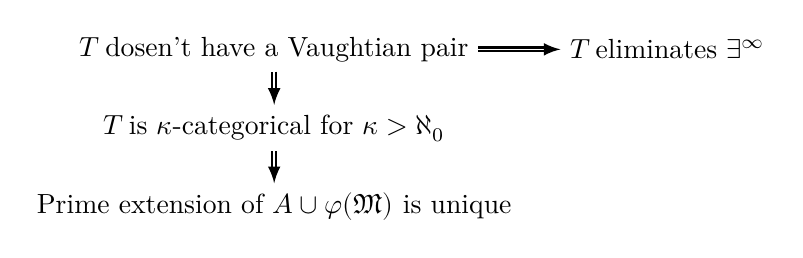
\begin{tikzpicture}
[a/.style={latex-latex,double,thick},
b/.style={-latex,thick,double}]
\node (1) {\(T\) dosen't have a Vaughtian pair};
\node (2) [below of=1]{\(T\) is \(\kappa\)-categorical for \(\kappa>\aleph_{0}\)};
\node (3) [below of=2]{Prime extension of \(A\cup\varphi(\fM)\) is unique};
\node (4) [right of=1,xshift=4cm]{\(T\) eliminates \(\exists^{\infty}\)};
\draw[b] (1) -- (2);
\draw[b] (1) -- (4);
\draw[b] (2) -- (3);
\end{tikzpicture}\end{center}

\begin{definition}[]
We say that \(T\) has a \textbf{Vaughtian pair} if there are two models \(\fM\prec\fN\) and
an \(L(M)\)-formula \(\varphi(x)\) s.t.
\begin{enumerate}
\item \(\fM\neq\fN\)
\item \(\varphi(\fM)\) is infinite
\item \(\varphi(\fM)=\varphi(\fN)\)
\end{enumerate}


If \(\varphi(x)\) doesn't contain parameters, we say that \(T\) has a Vaughtian pair for \(\varphi(x)\)
\end{definition}

\begin{remark}
Notice that \(T\) does not have a Vaughtian pair iff every model \(\fM\) is a minimal extension
of \(\varphi(\fM)\cup A\) for any formula \(\varphi(x)\) with parameters in \(A\subseteq M\) which defines an infinite
set in \(\fM\).
\wu{
If \(\fM\prec\fN\) is a Vaughtian pair and \(\varphi(\fM)=\varphi(\fN)\). Then as \(\fN\) is the minimal extension
of \(\varphi(\fM)\cup A\), \(\fN\prec\fM\) and thus we have an isomorphism
}
\end{remark}

Let \(\fN\) be a model of \(T\) where \(\varphi(\fN)\) is infinite but has smaller cardinality than \(\fN\).
The Löwenheim–Skolem Theorem yields an elementary substructure \(\fM\) of \(\fN\) which
contains \(\varphi(\fN)\) and has the same cardinality as \(\varphi(\fN)\). Then \(\fM\prec\fN\) is a Vaughtian pair
for \(\varphi(x)\). The next theorem shows that a converse of this observation is also true

\begin{theorem}[Vaught's Two-cardinal Theorem]
\label{thm5.5.2}
If \(T\) has a Vaughtian pair, it has a model \(\barfM\) of cardinality \(\aleph_1\)
with \(\varphi(\barfM)\) countable for some formula \(\varphi(x)\in L(\barM)\)
\end{theorem}

\begin{lemma}[]
\label{lemma5.5.3}
Let \(T\) be complete, countable and with infinite models
\begin{enumerate}
\item Every countable model of \(T\) has a countable \(\omega\)-homogeneous elementary extension
\item The union of an elementary chain of \(\omega\)-homogeneous models is \(\omega\)-homogeneous
\item Two \(\omega\)-homogeneous countable models of \(T\) realizing the same \(n\)-types for all \(n<\omega\)
are isomorphic
\end{enumerate}
\end{lemma}

\begin{proof}
\begin{enumerate}
\item Let \(\fM_0\) be a countable model of \(T\). We realise the countably many types
\begin{equation*}
\{f(\tp(a/A))\mid a,A\subseteq M_0,A\text{ finite},f:A\to M_0\text{ elementary}\}
\end{equation*}
in a countable elementary extension \(\fM_1\). By iterating this process we obtain an elementary
chain
\begin{equation*}
\fM_0\prec\fM_1\prec\cdots
\end{equation*}
whose union is \(\omega\)-homogeneous
\item Clear
\item Suppose \(\fA\) and \(\fB\) are \(\omega\)-homogeneous, countable and realise the same \(n\)-types. We
show that we can extend any finite elementary map \(f:\{a_1,\dots,a_i\}\to\{b_1,\dots,b_i\}\); \(a_j\mapsto b_j\) to
any \(a\in A\setminus A_i\). Realise the type \(\tp(a_1,\dots,a_i,a)\) by some
tuples \(\bbar{b'}=b_1',\dots,b_{i+1}'\) in \(B\).
\wu{
\(\tp^{\fA}(a_1,\dots,a_i,a)=\tp^{\fB}(\bbar{b'})\Rightarrow\tp^{\fB}(b_1,\dots,b_i)=\tp^{\fA}(a_1,\dots,a_i)=\tp^{\fB}(b_1',\dots,b_i')\).
}

Using the \(\omega\)-homogeneity of \(B\) we may extend
the finite partial isomorphism \(g=\{(b_j',b_j)\mid 1\le j\le i\}\) by \((b_{i+1}',b)\) for
some \(b\in B\). Then \(f_{i+1}=f_i\cup\{(a,b)\}\) is the required extension. Reverse the roles
of \(B\) and \(A\) we construct the desired isomorphism.
\end{enumerate}
\end{proof}

\begin{proof}[Proof of Theorem \ref{thm5.5.2}]
Suppose that the Vaughtian pair is witnessed (in certain models) by some formula \(\varphi(x)\). For
simplicity we assume that \(\varphi(x)\) does not contain parameters (see Exercise \ref{ex5.5.4}).
Let \(P\) be a new unary predicate. It is easy to find an \(L(P)\)-theory \(T_{\text{VP}}\) whose
models \((\fN,M)\) consist of a model \(\fN\vDash T\) and a subset \(M\) defined by the new
predicate \(P\) which is the universe of an elementary substructure \(\fM\) which together
with \(\fN\) forms a Vaughtian pair for \(\varphi(x)\).
\wu{
We can express the condition for Vaughtian pair in first-order language with \(P\):
\begin{enumerate}
\item \(\exists x(\neg P(x))\)
\item For each \(k>0\), \(\exists v_1\dots v_k(\bigwedge_{i<j}v_i\neq v_j\wedge\bigwedge\varphi(v_i))\)
\item \(\forall x(\varphi(x)\to P(x))\)
\end{enumerate}


And in addition, the elementary substructure
\begin{enumerate}
\setcounter{enumi}{3}
\item \(\forall\barv((\bigwedge_{i=1}^kP(v_i)\wedge\psi(\barv))\to\psi^P(\barv))\)
\end{enumerate}


As in Marker's p152. Let \(\fM\) be the elementary substructure of \(\fN\) by Löwenheim–Skolem Theorem .
}
The Löwenheim–Skolem Theorem applied to \(T_{\text{VP}}\) yields a Vaughtian pair \(\fM_0\prec\fN_0\)
for \(\varphi(x)\) with \(\fM_0,\fN_0\)  countable

We first construct an elementary chain
\begin{equation*}
(\fN_0,M_0)\prec(\fN_1,M_1)\prec\cdots
\end{equation*}
of countable Vaughtian pairs, with the aim that both components of the union pair
\begin{equation*}
(\fN,M)
\end{equation*}
are \(\omega\)-homogeneous and realise the same \(n\)-types. If \((\fN_i,M_i)\) is given, we first choose a
countable elementary extension \((\fN',M')\) s.t. \(\fM'\) realises all \(n\)-types which are
realised in \(\fN_i\).
\wu{
We only need to consider the 1-type. Then for each 1-type in \(\fN_i\), add a constant.
}
Then we choose as in the proof of Lemma
\ref{lemma5.5.3} a countable elementary extension \((\fN_{i+1},\fM_{i+1})\) of \((\fN',M')\) for
which \(\fN_{i+1}\) and \(\fM_{i+1}\) are \(\omega\)-homogeneous
\wu{
Prove: If \((\fN,M)\) is a countable \(\omega\)-homogeneous elementary extension of \((\fN',M')\), then both \(\fN\)
and \(\fM\) are homogeneous

Suppose \(\tp^{\fM}(\bara)=\tp^{\fM}(\barb)\) where \(\bara,\barb\in M^n\) and take \(a\in\fM\). For
any \(\varphi(\barx)\in\tp^{\fM}(\bara)\), \(\varphi(\barx)\in\tp^{(\fN,M)}(\bara)\) and
so \(\tp^{(\fN,M)}(\bara)=\tp^{(\fN,M)}(\barb)\). And there is \(b\in\fN\)
s.t. \(\tp^{(\fN,M)}(\bara,a)=\tp^{(\fN,M)}(\barb,b)\). But note
that \(\bigwedge_{i=1}^{n+1}P(x_i)\in\tp^{(\fN,M)}(\barb,b)\) and hence \(b\in M\).
}

It follows from Lemma \ref{lemma5.5.3} (3) that \(\fM\) and \(\fN\) are isomorphic
\wu{
since \(\fM\prec\fN\).
}

Next we construct a continuous elementary chain
\begin{equation*}
\fM^0\prec\fM^1\prec\cdots\prec\fM^\alpha\prec\cdots\quad(\alpha<\omega_1)
\end{equation*}
with \((\fM^{\alpha+1},\fM^\alpha)\cong(\fN,M)\) for all \(\alpha\). We start with \(\fM^0=\fM\). If \(\fM^\alpha\) is constructed, we
choose an isomorphism \(\fM\to\fM^\alpha\) and extend it to an isomorphism \(\fN\to\fM^{\alpha+1}\) (Lemma
\ref{lemma1.1.8}). For a countable limit ordinal \(\lambda\), \(\fM^\lambda\) is the union of the \(\fM^\alpha\) (\(\alpha<\lambda\)).
So \(\fM^\lambda\) is isomorphic to \(\fM\) by Lemma \ref{lemma5.5.3} (2) and \ref{lemma5.5.3} (3)

Finally we set
\begin{equation*}
\barfM=\bigcup_{\alpha<\omega_1}\fM^\alpha
\end{equation*}
\(\barfM\) has cardinality \(\aleph_1\) while \(\varphi(\barfM)=\varphi(\fM^\alpha)=\varphi(\fM^0)\).
\wu{
If \(\barfM\vDash\varphi(\bara)\), then  there is some \(\alpha<\omega_1\) s.t. \(\bara\in M^\alpha\cong M^0\).
}
\end{proof}

\begin{corollary}[]
\label{cor5.5.4}
If \(T\) is categorical in an uncountable cardinality, it does not have a Vaughtian pair
\end{corollary}

\begin{proof}
If \(T\) has a Vaughtian pair, then by Theorem \ref{thm5.5.2} it has a model \(\fM\) of
cardinality \(\aleph_1\) s.t. for some \(\varphi(x)\in L(M)\) the set \(\varphi(\fM)\) is countable. On the other
hand, if \(T\) is categorical in an uncountable cardinal, it is \(\aleph_1\)-categorical by Corollary
\ref{cor5.4.2} and by Theorem \ref{thm5.2.11}, all models of \(T\) of cardinality \(\aleph_1\) are
saturated. In particular, each formula is either satisfied by a finite number or by \(\aleph_1\) many
elements, a contradiction. \label{Problem2}
\end{proof}

\begin{corollary}[]
\label{cor5.5.5}
Let \(T\) be categorical in an uncountable cardinal, \(\fM\) a model, and \(\varphi(\fM)\) infinite and
definable over \(A\subseteq M\). Then \(\fM\) is the unique prime extension of \(A\cup\varphi(\fM)\)
\end{corollary}

\begin{proof}
By Corollary \ref{cor5.5.4}, \(T\) does not have a Vaughtian pair, so \(\fM\) is minimal
over \(A\cup\varphi(\fM)\). If \(\fN\) is a prime extension
\end{proof}

\begin{definition}[]
We say that \(T\) \textbf{eliminates the quantifier \(\exists^\infty x\) (there are infinitely many \(x\))}, if for
every \(L\)-formula \(\varphi(x,\bary)\) there is a finite bound \(n_\varphi\) s.t. in all models \(\fM\)
of \(T\) and for all parameters \(\bara\in M\)
\begin{equation*}
\varphi(\fM,\bara)
\end{equation*}
is either infinite or has at most \(n_\varphi\) elements
\end{definition}

\begin{remark}
This means that for all \(\varphi(x,\bary)\) there is a \(\psi(\bary)\) s.t. in all models \(\fM\) of \(T\)
and for all \(\bara\in M\)
\begin{equation*}
\fM\vDash\exists^\infty x\varphi(x,\bara)\Longleftrightarrow\fM\vDash\psi(\bara)
\end{equation*}
We denote this by
\begin{equation*}
T\vDash\forall\bary\left( \exists^\infty x\varphi(x,\bary)\leftrightarrow\psi(\bary) \right)
\end{equation*}
\end{remark}

\begin{proof}
If \(n_\varphi\) exists, we can use \(\psi(\bary)=\exists^{>n_{\varphi}}x\varphi(x,\bary)\). If conversely \(\psi(\bary)\) is
a formula which is implied by \(\exists^\infty x\varphi(x,\bary)\), a compactness argument shows that there must
be a bound \(n_\varphi\) s.t.
\begin{equation*}
T\vDash\exists^{>n_\varphi}x\varphi(x,\bary)\to\psi(\bary)
\end{equation*}
\wu{
First note that \(T\) is complete. If there is no such bound, then for
any \(n\in\N\), \(T\not\vDash\exists^{>n}x\varphi(x,\bary)\to\psi(\bary)\), which is
\(T\vDash\exists^{>n}x\varphi(x,\bary)\wedge\neg\psi(\bary)\). Thus by compactness \(T\vDash\exists^\infty x\varphi(x,\bary)\wedge\neg\psi(\bary)\), a contradiction.
}
\end{proof}

\begin{lemma}[]
\label{lemma5.5.7}
A theory \(T\) without Vaughtian pair eliminates the quantifier \(\exists^\infty x\)
\end{lemma}

\wu{
Check Marker's Lemma 4.3.37 and Lemma 6.1.14
}

\begin{proof}
Let \(P\) be a new unary predicate and \(c_1,\dots,c_n\) new constants. Let \(T^*\) be the theory
\wu{
Check Marker's Lemma 6.1.14 to see the the formal version
}
of all \(L\cup\{P,c_1,\dots,c_n\}\)-structures
\begin{equation*}
(\fM,N,a_1,\dots,a_n)
\end{equation*}
where \(\fM\) is a model of \(T\), \(N\) is the universe of a proper elementary substructure,
 \(a_1,\dots,a_n\) elements of \(N\) and \(\varphi(\fM,\bara)\subseteq N\).
Suppose that the
bound \(n_\varphi\) does not exists. Then, for any \(n\), there is a model \(\fN\) of \(T\)
and \(\bara\in N\) s.t. \(\varphi(\fN,\bara)\) is finite, but has more than \(n\) elements. Let \(\fM\) be a
proper elementary extension of \(\fN\).
Then \(\varphi(\fM,\bara)=\varphi(\fN,\bara)\)
\wu{
(as \(\varphi(\fN,\bara)\) is finite, we can add formulas to ensure this)
}
and the pair \((\fM,N,\bara)\) is a model of \(T^*\). This shows
that the theory
\begin{equation*}
T^*\cup\{\exists^{>n}x\varphi(x,\barc)\mid n=1,2,\dots\}
\end{equation*}
is finitely satisfiable. A model of this theory gives a Vaughtian pair for \(T\).
\end{proof}

\begin{exercise}
\label{ex5.5.1}
If \(T\) is totally transcendental and has a Vaughtian pair for \(\varphi(x)\), then it has, for all
uncountable \(\kappa\), a model of cardinality \(\kappa\) with countable \(\varphi(\fM)\).
\end{exercise}

\begin{proof}
Marker's Theorem 4.3.41
\end{proof}

\begin{exercise}
\label{ex5.5.4}
Let \(T\) be a theory, \(\fM\) a model of \(T\) and \(\bara\subseteq M\) a finite tuple of parameters.
Let \(q(\barx)\) be the type of \(\bara\) in \(\fM\). Then for new constants \(\barc\),
the \(L(\barc)\)-theory
\begin{equation*}
T(q)=\Th(\fM,\bara)=T\cup\{\varphi(\barc)\mid\varphi(\barx)\in q(\barx)\}
\end{equation*}
is complete. Show that \(T\) is \(\lambda\)-stable (or without Vaughtian pair etc.) iff \(T(q)\) is. For
countable languages this implies that \(T\) is categorical in some uncountable cardinal
iff \(T(q)\) is.
\end{exercise}

\begin{proof}
If \(T\) is \(\lambda\)-stable and \(\fN,\barb\vDash T(q)\), then there is an partial elementary map
\(f:\bara\to\barb\) from \(\fM\) to \(\fN\). By Marker's Corollary 4.1.7, we can extend \(f\) to an
elementary map \(f':\fM\to\fN'\) where \(\fN\prec\fN'\).
\end{proof}

\subsection{Algebraic formulas}
\label{sec:org3817a45}
\begin{definition}[]
Let \(\fM\) be a structure and \(A\) a subset of \(M\). A formula \(\varphi(x)\in L(A)\) is called
\textbf{algebraic} if \(\varphi(\fM)\) is finite. An element \(a\in M\) is algebraic over \(A\) if it realizes an
algebraic \(L(A)\)-formula. We call an element algebraic if it is algebraic over the empty set.
The \textbf{algebraic closure} of \(A\), \(\acl(A)\), is the set of all elements of \(\fM\) algebraic
over \(A\), and \(A\) is called \textbf{algebraically closed} if it equals its algebraic closure
\end{definition}

\begin{remark}
Note that the algebraic closure of \(A\) does not grow in elementary extensions of \(\fM\) because
an \(L(A)\)-formula which defines a finite set in \(\fM\) defines the same set in every elementary
extension
\wu{
We can express there are exactly \(m\) solutions in formula.
}
\end{remark}

By Theorem \ref{thm2.3.1}
\begin{equation*}
\abs{\acl(A)}\le\max(\abs{T},\abs{A})
\end{equation*}
In algebraically closed fields, an element \(a\) is algebraic over \(A\) precisely if \(a\) is
algebraic (in the field-theoretical sense) over the field generated by \(A\). This follows from
quantifier elimination in \(\ACF\)

We call a type \(p(x)\in S(A)\) algebraic iff \(p\) contains an algebraic formula. Any algebraic
type \(p\) is isolated by an algebraic formula \(\varphi(x)\in L(A)\), namely by any \(\varphi\in p\) having the
minimal number of solutions in \(\fM\).
\wu{
Suppose \(\psi\in p\) is algebraic. If \(\psi\) doesn't isolate \(p\). Then there is \(\phi\in p\)
s.t. \(\phi\wedge\psi(\fM)\) is a proper subset of \(\psi(\fM)\). This process will end since \(\psi\) is algebraic
}
This number is called the \textbf{degree} \(\deg(p)\) of \(p\). As isolated types are realised in every
model, the algebraic types over \(A\) are exactly of the form \(\tp(a/A)\) where \(a\) is
algebraic over \(A\). The \textbf{degree} of \(a\) over \(A\) \(\deg(a/A)\) is the degree of \(\tp(a/A)\).

\begin{lemma}[]
\label{lemma5.6.2}
Let \(p\in S(A)\) be non-algebraic and \(A\subseteq B\). Then \(p\) has a non-algebraic extension \(q\in S(B)\).
\end{lemma}

\begin{proof}
The extension \(q_0(x)=p(x)\cup\{\neg\psi(x)\mid\psi(x)\text{ algebraic }L(B)\text{-formula}\}\) is finitely
satisfiable. For otherwise there are \(\varphi(x)\in p(x)\)
\wu{
( \(p\) is a type and is closed under conjunction)
}
and algebraic \(L(B)\)-formulas \(\psi_1(x),\dots,\psi_n(x)\) with
\begin{equation*}
\fM\vDash\forall x(\varphi(x)\to\psi_1(x)\vee\dots\vee\psi_n(x))
\end{equation*}
But then \(\varphi(x)\)
\wu{
(\(\varphi(x)\) has finitely many solutions)
}
and hence \(p(x)\) is algebraic. So we can take for \(q\) any type containing \(q_0\).
\end{proof}

\begin{remark}
\label{re5.6.3}
Since algebraic types are isolated by algebraic formulas, an easy compactness argument shows that
a type \(p\in S(A)\) is algebraic iff \(p\) has only finitely many realisations (namely \(\deg(p)\)
many) in all elementary extensions of \(\fM\).
\end{remark}

\begin{proof}
\(\Rightarrow\). Obvious.

\(\Leftarrow\). Suppose \(p\in S(A)\) is not algebraic in \(\fM\). Add infinitely many constants \(C\), for
any \(\varphi\in p\), let \(\Phi=\{\varphi(c):c\in C\}\) and
\begin{equation*}
 \Gamma=\Diag_{\el}(\fM)\cup\{c\neq d:c,d\in C\}\cup\bigcup\{\Phi:\varphi\in p\}
\end{equation*}
Then \(\Gamma\) is finitely satisfied by \(\fM\) and we have a model where \(p\) has infinitely many realisations
\end{proof}

\begin{lemma}[]
\label{lemma5.6.4}
Let \(\fM\) and \(\fN\) be two structures and \(f:A\to B\) an elementary bijection between two subsets.
Then \(f\) extends to an elementary bijection between \(\acl(A)\) and \(\acl(B)\)
\end{lemma}

\begin{proof}
Let \(g:A'\to B'\) a maximal extension of \(f\) to two subsets of \(\acl(A)\) and \(\acl(B)\).
Let \(a\in \acl(A)\). Since \(a\) is algebraic over \(A'\), \(a\) is atomic over \(A'\). We can
therefore realise the type \(g(\tp(a/ A'))\) in \(\fN\) - by an element \(b\in\acl(B)\) - and obtain
an extension \(g\cup\{\la a,b\ra\}\) of \(g\). It follows that \(a\in A'\). So \(g\) is defined on the
whole \(\acl(A)\). Interchanging \(A\) and \(B\) shows that \(g\) is surjective
\end{proof}

\begin{definition}[]
A \textbf{pregeometry} (or \textbf{matroid}) \((X,\cl)\) is a set \(X\) with a closure operator \(\cl:\calp(X)\to\calp(X)\)
where \(\calp\) denotes the power set, s.t. for all \(A\subseteq X\) and \(a,b\in X\)
\begin{enumerate}
\item (REFLEXIVITY) \(A\subseteq\cl(A)\)
\item (FINITE CHARACTER) \(\cl(A)\) is the union of all \(\cl(A')\), where the \(A'\) range over all
finite subsets of \(A\)
\item (TRANSITIVITY) \(\cl(\cl(A))=\cl(A)\)
\item (EXCHANGE) \(a\in\cl(Ab)\setminus\cl(A)\Rightarrow b\in\cl(Aa)\)
\end{enumerate}
\end{definition}

A set \(A\) is called \textbf{closed} if \(A=\cl(A)\).

\begin{lemma}[]
If \(X\) is the universe of a structure, \(\acl\) satisfies REFLEXIVITY, FINITE CHARACTER and TRANSITIVITY
\end{lemma}

\subsection{Strongly minimal sets}
\label{sec:org496bcd2}
We fix a complete theory \(T\) with infinite models.
\begin{definition}[]
Let \(\fM\) be a model of \(T\) and \(\varphi(\barx)\) a non-algebraic \(L(M)\)-formula
\begin{enumerate}
\item The set \(\varphi(\fM)\) is called \textbf{minimal in \(\fM\)} if for all \(L(M)\)-formulas \(\psi(\barx)\) the
intersection \(\varphi(\fM)\wedge\psi(\fM)\) is either finite or cofinite in \(\varphi(\fM)\)
\item The formula \(\varphi(\barx)\)p is \textbf{strongly minimal} if \(\varphi(\barx)\) defines a minimal set in all
elementary extensions of \(\fM\). In this case, we also call the definable set \(\varphi(\fM)\)
strongly minimal. A \uline{non-algebraic} type containing a strongly minimal formula is called
strongly minimal
\item A theory \(T\) is strongly minimal if the formula \(x\dot=x\) is strongly minimal
\end{enumerate}
\end{definition}

Strong minimality is preserved under definable bijections; i.e., if \(A\) and \(B\) are
definable subsets of \(\fM^k\), \(\fM^m\) defined by \(\varphi\) and \(\psi\), respectively, s.t. there is a definable
bijection between \(A\) and \(B\), then if \(\varphi\) is strongly minimal so is \(\psi\).
\wu{
Suppose bijection \(f(\bara)=\barb\) iff \(\gamma(\bara,\barb)\). Then for any \(\theta(\barx)\), we have \(\theta'(\bary)=\exists\barx(\theta(\barx)\wedge\gamma(\barx,\bary))\)
}

\begin{examplle}[]
\begin{enumerate}
\item The following theories are strongly minimal, which is easily seen in each case using
quantifier elimination
\begin{itemize}
\item \(\Infset\). The sets which are definable over a parameter set \(A\) in a model \(M\) are
the finite subsets \(S\) of \(A\) and their completements \(M\setminus S\)
\item For a field \(K\), the theory of infinite \(K\)-vector spaces. The sets definable over a
set \(A\) are the finite subsets of the subspace spanned by \(A\) and their complements
\label{Problem3}
\wu{
\(K\) is divided by the subspace spanned by \(A\) and its complement.
}
\item The theories \(\ACF_p\). The definable sets of any model \(K\) are Boolean combinations of
zero-sets
\begin{equation*}
\{a\in K\mid f(a)=0\}
\end{equation*}
of polynomials \(f(X)\in K[X]\). Zero-sets are finite, or if \(f=0\), all of \(K\).
\wu{
\(f(x)\neq 0\) is cofinite
}.
\end{itemize}
\item If \(K\vDash\ACF_p\) , for any \(a,b\in K\), the formula \(ax_1+b=x_2\) defining an affine line \(A\)
in \(K^2\) is strongly minimal as there is a definable bijection between \(A\) and \(K\).
\wu{
The formula defines a map
}
\item For any strongly minimal formula \(\varphi(x_1,\dots,x_n)\), the \textbf{induced theory} \(T\restriction\varphi\) is
strongly minimal. Here, for any \(\fM\vDash T\), the induced theory is the theory of \(\varphi(\fM)\) with
the structure given by all intersections of 0-definable subsets of \(M^{nm}\) with \(\varphi(\fM)^m\)
for all \(m\in\omega\). This theory depends only on \(T\) and \(\varphi\), not on \(\fM\). \label{Problem4}
\end{enumerate}
\end{examplle}

Whether p\(\varphi(\barx,\bara)\) is strongly minimal depends only on the type of the parameter
tuple \(\bara\) and not on the actual model: observe that \(\varphi(\barx,\bara)\) is strongly minimal
iff for all \(L\)-formulas \(\psi(\barx,\barz)\) the set
\begin{align*}
\Sigma_\psi(\barz,\bara)=\{\exists^{>k}\barx(\varphi(\barx,\bara)\wedge&\psi(\barx,\barz))\wedge\\
&\exists^{>k}\barx(\varphi(\barx,\bara)\wedge\neg\psi(\barx,\barz))\mid k=1,2,\dots\}
\end{align*}
cannot be realised in any elementary extension. This means that for all \(\psi(\barx,\barz)\) there
is a bound \(k_\psi\) s.t.
\begin{equation*}
\fM\vDash\forall\barz(\exists^{\le k_\psi}\barx(\varphi(\barx,\bara)\wedge\psi(\barx,\barz))\vee\exists^{\le k_\psi}(\varphi(\barx,\bara)\wedge\neg\psi(\barx,\barz)))
\end{equation*}
This is an \textbf{elementary property} of \(\bara\), i.e., expressible by a first-order formula. So it
makes sense to call \(\varphi(\barx,\bara)\) a strongly minimal formula without specifying a model

\wu{
Note that in our definition, \(\varphi(\barx)\) a non-algebraic \(L(M)\)-formula. Thus from our
definition, \(\varphi(\barx,\bara)\in L(A)\) is strongly minimal as long as it has such elementary which is
required for all elementary extensions of \(\fA\). Guess this is the BASE model of all elementary
extensions.

One consequence is, we only need to say \(\abs{\varphi(\fC)}>k_\varphi\)  to say \(\abs{\varphi(\fC)}\) is infinite.
Just like we eliminate the \(\exists^\infty\)
}

\begin{lemma}[]
\label{lemma5.7.2}
If \(\fM\) is \(\omega\)-saturated, or if \(T\) eliminates the quantifier \(\exists^\infty\), any minimal formula is
strongly minimal. If \(T\) is totally transcendental, every infinite definable subset of \(\fM^n\)
contains a minimal set \(\varphi(\fM)\).
\end{lemma}

\begin{proof}
If \(\fM\) is \(\omega\)-saturated and \(\varphi(\barx,\bara)\) not strongly minimal, then for
some \(L\)-formula \(\psi(\barx,\barz)\) the set \(\Sigma_\psi(\barz,\bara)\) is realised in \(\fM\), so \(\varphi\) is not minimal.

If on the other hand \(\varphi(\barx,\bara)\) is minimal and \(T\) eliminates the quantifier \(\exists^\infty\),
then for all \(L\)-formulas \(\psi(\barx,\barz)\)
\begin{equation*}
\neg(\exists^\infty\barx(\varphi(\barx,\bara)\wedge\psi(\barx,\barz))\wedge\exists^\infty\barx(\varphi(\barx,\bara)\wedge\neg\psi(\barx,\barz)))
\end{equation*}
is an elementary property of \(\barz\).
\wu{
If we can eliminate \(\exists^\infty\), then we can express minimality by a first-order sentence. Thus it's
strongly minimal.
Guess the power of infinitary disjunction \emoji{😅}
}

If \(\varphi_0(\fM)\) does not contain a minimal set, one can construct from \(\varphi_0(\barx)\) a binary
tree of \(L(M)\)-formulas defining infinite subsets of \(\fM\).
\wu{
As \(\varphi_0(\fM)\) does not contain a minimal set, its not minimal?

If \(\varphi(\fM)\) is not minimal, then there is an \(L(M)\)-formula \(\psi(\barx)\) and
both \(\varphi(\fM)\wedge\psi(\fM)\) and \(\varphi(\fM)\wedge\neg\psi(\fM)\) are infinite and not minimal. Thus we can construct a
binary tree from this.
}
\end{proof}

From now on we will only consider strongly minimal formulas in one variable.

\begin{lemma}[]
\label{lemma5.7.3}
The formula \(\varphi(\fM)\) is minimal iff there is a unique non-algebraic type \(p\in S(M)\) containing \(\varphi(x)\)
\end{lemma}

\begin{proof}
If \(\varphi(\fM)\) is minimal, then clearly
\begin{equation*}
p=\{\psi\mid\psi(x)\in L(M)\text{ s.t. }\varphi\wedge\neg\psi\text{ is algebraic}\}
\end{equation*}
is the unique non-algebraic type in \(S(M)\) containing it.
\wu{
\(\varphi(x)\) is minimal iff for any \(\psi(x)\in L(M)\), \(\varphi\wedge\psi\) or \(\varphi\wedge\neg\psi\)  is algebraic.. Guess algebraic
requires \(\abs{\varphi(\fM)}>0\).

if there is another non-algebraic type \(q\in S(M)\) and we take \(\gamma(x)\in q\setminus p\). Then \(\gamma\wedge\varphi\in q\)
and hence \(\varphi\wedge\neg\gamma\) is algebraic. Thus \(\gamma\in p\)
}

If \(\varphi(\fM)\) is not minimal, there is some \(L\)-formula \(\psi\) with both \(\varphi\wedge\psi\) and \(\varphi\wedge\neg\psi\)
non-algebraic. By Lemma \ref{lemma5.6.2}, there are at least two non-algebraic types in \(S(M)\)
containing \(\varphi\).
\end{proof}

\begin{corollary}[]
\label{cor5.7.4}
A strongly minimal type \(p\in S(A)\) has a unique non-algebraic extension to all supersets \(B\)
of \(A\) in an elementary extensions of \(\fM\). Consequently, the type of \(m\)
realisations \(a_1,\dots,a_m\) of \(p\) with \(a_i\notin\acl(a_1,\dots,a_{i-1}A)\), \(i=1,\dots,m\) is uniquely determined.
\end{corollary}

\begin{proof}
Existence of non-algebraic extensions follows from Lemma \ref{lemma5.6.2}, which also allows us to
assume that \(B\) is a model.

Uniqueness follows from Lemma \ref{lemma5.7.3} applied to any strongly minimal formula of \(p\).
The last sentence follows by induction.

\label{Problem6}
\wu{
See Marker's Lemma 6.1.6. Thus \(p\) is strongly minimal in the problem.

First we need to prove that for any \(a,b\notin\acl(A)\), \(\tp(a/A)=\tp(b/A)\). As \(p\) is strongly
minimal, there is a strongly minimal formula \(\phi(x)\in p(x)\). For any \(\fM\vDash\psi(a)\),
as \(\phi(a)\wedge\psi(a)\), \(\phi(\fM)\wedge\psi(\fM)\) is infinite, and thus \(\phi(\fM)\wedge\neg\psi(\fM)\) is finite. As \(\fM\vDash\phi(b)\),
we have \(b\notin\phi(\fM)\wedge\neg\psi(\fM)\) and hence \(\fM\vDash\phi(b)\wedge\psi(b)\). Consequently, \(\tp(a/A)=\tp(b/A)\).

Inductive step is similar

}
\end{proof}

\begin{theorem}[]
\label{thm5.7.5}
\label{Problem7}
If \(\varphi(x)\) is strongly minimal formula in \(\fM\) without parameters, the operation
\begin{equation*}
\cl:\fP(\varphi(\fM))\to\fP(\varphi(\fM))
\end{equation*}
defined by
\begin{equation*}
\cl(A)=\acl^M(A)\cap\varphi(\fM)
\end{equation*}
is a pregeometry \((\varphi(\fM),\cl)\)
\end{theorem}

\begin{proof}
We have to verify EXCHANGE.
\wu{
Prove \(a\in\cl(Ab)\setminus\cl(A)\Rightarrow b\in\cl(Aa)\).
}
For notational simplicity we assume \(A=\emptyset\).
\wu{
Now we prove \(a\in\cl(b)\setminus\cl(\emptyset)\Rightarrow b\in\cl(a)\).
}
Let \(a\in\varphi(\fM)\) be not algebraic over \(\emptyset\) and \(b\in\varphi(\fM)\) not algebraic over \(a\).
\wu{
(Prove by contradiction)
}
By Corollary \ref{cor5.7.4}, all such pairs \(a,b\) have the same type \(p(x,y)\). Let \(A'\) be
an infinite set of non-algebraic elements realising \(\varphi\) (which exists in an elementary extension
of \(\fM\))
\wu{
\(a\) is non-algebraic that realising \(\varphi\) iff for any \(\psi\) that cofinite in \(\varphi\), \(a\in\bigcap\varphi(\fM)\wedge\psi(\fM)\).

If \(\varphi(\fM)\wedge\psi(\fM)\) and \(\varphi(\fM)\wedge\theta(\fM)\) are infinite, then either \((\varphi\wedge\psi\wedge\theta)(\fM)\) is infinite
or \((\varphi\wedge\neg(\psi\wedge\theta))(\fM)\) is infinite. But \(\varphi\wedge\neg(\psi\wedge\theta)=(\varphi\wedge\neg\psi)\vee(\varphi\wedge\neg\theta)\), thus it's finite and
\((\varphi\wedge\psi\wedge\theta)(\fM)\) is infinite. Hence \(\{\varphi\}\cup\{\psi:(\varphi\wedge\psi)(\fM)\text{ infinite}\}\) is finitely satisfiable and
thus satisfiable.

Then we just add constants satisfying these formulas. This is an elementary extension by Tarski test.
}
and \(b'\) non-algebraic over \(A'\).
\wu{
\(\varphi\) is strongly minimal and we can view \(A'\) as some extensions
}
Since all \(a'\in A'\) have the same
type \(p(x,b')\) over \(b'\), no \(a'\) is algebraic over \(b'\).
\wu{
\(a'\) is algebraic over \(b'\) iff there is \(\fM\vDash\varphi(a',b')\) s.t. \(\varphi(\fM,b')\) is finite. But for
all \(a',a''\in A'\), \(\tp(a',b')=\tp(a'',b')\). Thus \(\abs{\varphi(\fM,b')}\ge\abs{\varphi(A')}\).
}
Thus also \(a\) is not
algebraic over \(b\).
\end{proof}

The same proof shows that algebraic closure defines a pregeometry on the set of realizations of
a \emph{minimal} type, i.e., a non-algebraic type \(p\in S_1(A)\) having a unique non-algebraic extension
to all supersets \(B\) of \(A\) in elementary extensions of \(\fM\). Here is an example to show
that a minimal type need not be strongly minimal

Let \(T\) be the theory of \(\fM=(M,P_i)_{i<\omega}\) in which the \(P_i\) form a proper descending
sequence of subsets. The type \(p=\{x\in P_i\mid i<\omega\}\in S_1(\emptyset)\) is minimal. If all \(P_{i+1}\) are
cofinite in \(P_i\), then \(p\) does not contain a minimal formula and is not strongly minimal

In pregeometries there is a natural notion of independence and dimension, so in light of Theorem
\ref{thm5.7.5} , we may define the following

If \(\varphi(x)\) is strongly minimal without parameters, the \textbf{\(\varphi\)-dimension} of a model \(\fM\)
of \(T\) is the dimension of the pregeometry \((\varphi(\fM),\cl)\)
\begin{equation*}
\dim_\varphi(\fM)
\end{equation*}
If \(\fM\) is the model of a strongly minimal theory, we just write \(\dim(\fM)\)

If \(\varphi(x)\) is defined over \(A_0\subseteq M\), the closure operator of the pregeometry \(\varphi(\fM_{A_0})\)
is given by
\begin{equation*}
\cl(A)=\acl^M(A_0\cup A)\cap\varphi(\fM)
\end{equation*}
and
\begin{equation*}
\dim_\varphi(\fM/A_0):=\dim_{\varphi}(\fM_{A_0})
\end{equation*}
is called the \(\varphi\)-dimension of \(\fM\) over \(A_0\).

\begin{lemma}[]
\label{lemma5.7.6}
Let \(\varphi(x)\) be defined over \(A_0\) and strongly minimal, and let \(\fM\) and \(\fN\) be models
containing \(A_0\). Then there exists an \(A_0\)-elementary map between \(\varphi(\fM)\) and \(\varphi(\fN)\)
iff \(\fM\) and \(\fN\) have the same \(\varphi\)-dimension over \(A_0\)
\end{lemma}

\begin{proof}
An \(A_0\)-elementary map between \(\varphi(\fM)\) and \(\varphi(\fN)\) maps bases to bases, so one direction is
clear

For the other direction we use Corollary \ref{cor5.7.4}: if \(\varphi(\fM)\) and \(\varphi(\fN)\) have the same
dimension over \(A_0\), let \(U\) and \(V\) be bases of \(\varphi(\fM)\) and \(\varphi(\fN)\), respectively, and
let \(f:U\to V\) be a bijection. By Corollary \ref{cor5.7.4}, \(f\) is \(A_0\)-elementary
\wu{
The are indiscernibles.
}
and by Lemma \ref{lemma5.6.4} \(f\) extends to an elementary
bijection \(g:\acl(A_0U)\to\acl(A_0V)\). Thus \(g\upharpoonright\varphi(\fM)\) is an \(A_0\)-elementary map
from \(\varphi(\fM)\) to \(\varphi(\fN)\)
\end{proof}

\begin{corollary}[]
\label{cor5.7.7}
\begin{enumerate}
\item A theory \(T\) is strongly minimal iff over every parameter set there is exactly one
non-algebraic type
\item In models of a strongly minimal theory the algebraic closure defines a pregeometry
\item Bijections between independent subsets of models of a strongly minimal theory are elementary.
In particular, the type of \(n\) independent elements is uniquely determined
\end{enumerate}
\end{corollary}

\begin{proof}
\begin{enumerate}
\item Lemma \ref{lemma5.7.3}
\item From Theorem \ref{thm5.7.5}
\end{enumerate}
\end{proof}

If \(T\) is strongly minimal, by the preceding we have
\begin{equation*}
\abs{S(A)}\le\abs{\acl(A)}+1
\end{equation*}
\wu{
1 is for the unique non-algebraic type. Every algebraic type \(p\) is isolated by \(\varphi_p(x)\).
Also \(\varphi(\fM)\subseteq\acl(A)\). For different \(\varphi_p\) and \(\varphi_q\), \(\varphi_p(\fM)\neq\varphi_q(\fM)\). So different algebraic \(p\)
is at least realized by one unique element.
}
Strongly minimal theories are therefore \(\lambda\)-stable for all \(\lambda\ge\abs{T}\)
\wu{
as \(\abs{\acl(A)}\le\max(\abs{T},\abs{A})\).
}
Also there can be no binary tree of finite or cofinite sets. So by the remark after the proof of
Theorem \ref{thm5.2.6} \(T\) is totally transcendental
\wu{
as we restrict \(\varphi\) to one variable.
}
. If \(\varphi(\fM)\) is cofinite and \(\fN\) a proper
elementary extension of \(\fM\), then \(\varphi(\fN)\) is a proper extension of \(\varphi(\fM)\)
\wu{
as \(\abs{\fM-\varphi(\fM)}\) is fixed.
}
Thus strongly minimal theories have no Vaughtian pairs.

\begin{theorem}[]
\label{thm5.7.8}
Let \(T\) be strongly minimal. Models of \(T\) are uniquely determined by their dimensions. The
set of possible dimensions is an end segment of the cardinals. A model \(\fM\) is \(\omega\)-saturated
iff \(\dim(\fM)\ge\aleph_0\). All models are \(\omega\)-homogeneous
\end{theorem}

\begin{proof}
Let \(\fM_0,\fM_1\) be models of the same dimension, and let \(B_0,B_1\) be bases for \(\fM_0\)
and \(\fM_1\), respectively. Then any bijection \(f:B_0\to B_1\) is an elementary map by Corollary
\ref{cor5.7.7}, which extends to an isomophism of the algebraic closure \(\fM_0\) and \(\fM_1\) by
Lemma \ref{lemma5.6.4}

\textbf{Claim}. Every infinite algebraically closed subset \(S\) of \(M\) is the universe of an
 elementary substructure

\emph{Proof}. By Theorem \ref{thm2.1.2} it suffices to show that every
consistent \(L(S)\)-formula \(\varphi(x)\) can be realised in \(S\). If \(\varphi(\fM)\) is finite, all
realisations are algebraic over \(S\) and belong to \(S\). If \(\varphi(\fM)\) is cofinite, \(\varphi(\fM)\)
meets all infinite sets.

Let \(A\) be a finite subset of \(\fM\) and \(p\) the non-algebraic type in \(S(A)\).
\wu{
Suppose there are i guess. Since all algebraic types are isolated.
}
Thus \(p\) is realised in \(\fM\) exactly if \(M\neq\acl(A)\)
\wu{
Note that for any \(\varphi\in p\), \(\varphi(\fM)\) is cofinite. If \(p\) is not realised,
then \(\bigcup_{\varphi\in p}(\neg\varphi)(\fM)=\fM\) and every element of \(\fM\) is algebraic over \(A\).
}
i.e., iff \(\dim(\fM)>\dim(A)\). Since
all algebraic types over \(A\) are always realised in \(\fM\), this shows that \(\fM\) is
\(\omega\)-saturated iff \(\fM\) has infinite dimension.

Let \(f:A\to B\) be an elementary bijection between two finite subsets of \(M\). By Lemma
\ref{lemma5.6.4}, \(f\) extends to an elementary bijection between \(\acl(A)\) and \(\acl(B)\).
If \(a\in M\setminus\acl(A)\), then \(p=\tp(a/A)\) is the unique
\wu{
Corollary \ref{cor5.7.4}
}
non-algebraic type over \(A\)
 and \(f(p)\) is the unique non-algebraic type over \(B\). Since \(\dim(A)=\dim(B)\), the
 argument in the previous paragraph shows that \(f(p)\) is realised in \(\fM\)
\wu{
As \(M\setminus\acl(A)\neq\emptyset\), \(\dim(\fM)>\dim(A)\)
}
\end{proof}

\begin{corollary}[]
If \(T\) is countable and strongly minimal, it is categorical in all uncountable cardinalities
\end{corollary}

\begin{proof}
Let \(\fM_1\) and \(\fM_2\) be two models of cardinality \(\kappa>\aleph_0\). Choose two bases \(B_1\) and \(B_2\)
of \(\fM_1\) and \(\fM_2\) respectively. Then \(B_1\) and \(B_2\) both have cardinality \(\kappa\)
as \(\abs{\acl(A)}\le\max(\abs{T},\abs{A})\). Then any
bijection \(f:B_1\to B_2\) is an elementary map by Corollary \ref{cor5.7.7}, which extends to an
isomophism of the algebraic closures \(M_1\) and \(M_2\) by Lemma \ref{lemma5.6.4}
\end{proof}

\begin{exercise}
\label{ex5.7.1}
If \(\fM\) is minimal and \(\omega\)-saturated, then \(\Th(\fM)\) is strongly minimal
\end{exercise}


\subsection{The Baldwin-Lachlan Theorem}
\label{sec:org31e8c17}
\begin{theorem}[Baldwin-Lachlan]
Let \(\kappa\) be an uncountable cardinal. A countable theory \(T\) is \(\kappa\)-categorical iff \(T\) is
\(\omega\)-stable and has no Vaughtian pairs
\end{theorem}

\begin{proof}
If \(T\) is categorical in some uncountable cardinal, then \(T\) is \(\omega\)-stable by Theorem
\ref{thm5.2.4} and has no Vaughtian pair by Corollary \ref{cor5.5.4}.

For the other direction we first obtain a strongly minimal formula: since \(T\) is totally
transcendental, it has a prime model \(\fM_0\). (This follows from Theorems \ref{thm4.5.7} and
\ref{thm4.5.9} or from Theorem \ref{thm5.3.3}) Let \(\varphi(x)\) be a minimal formula in \(L(M_0)\),
which exists by Lemma \ref{lemma5.7.2}. Since \(T\) has no Vaughtian pairs, \(\exists^\infty\) can be
eliminated by Lemma \ref{lemma5.5.7} and hence \(\varphi(x)\) is strongly minimal by Lemma
\ref{lemma5.7.2}.

Let \(\fM_1,\fM_2\) be models of cardinality \(\kappa\). We may assume that \(\fM_0\) is an elementary submodel
of both \(\fM_1\) and \(\fM_2\)
\wu{
as \(\fM_0\) is prime.
}
Since \(T\) has no Vaughtian pair, \(\fM_i\) is a minimal extension of \(M_0\cup\varphi(\fM_i)\), \(i=1,2\).
Therefore \(\varphi(\fM_i)\) has cardinality \(\kappa\)
\wu{
\(M_0\) is prime model and thus is countable since \(T\).
}
and hence we conclude
that \(\dim_\varphi(\fM_1/M_0)=\kappa=\dim_\varphi(\fM_2/M_0)\). By Lemma \ref{lemma5.7.6} there exists
an \(M_0\)-equivalent map from \(\varphi(\fM_0)\) to \(\varphi(\fM_1)\), which by Lemma \ref{lemma5.3.8} extends to
an isomorphism from \(\fM_1\) to \(\fM_2\)
\end{proof}

\begin{corollary}[]
Let \(\kappa\) be an uncountable cardinal. Then \(T\) is \(\aleph_1\)-categorical iff \(T\) is \(\kappa\)-categorical
\end{corollary}

\begin{corollary}[]
Suppose \(T\) is \(\aleph_1\)-categorical, \(\fM_1,\fM_2\) are models of \(T\), \(a_i\in\fM_i\) and \(\varphi(x,a_i)\)
strongly minimal, \(i=1,2\), with \(\tp(a_1)=\tp(a_2)\). If \(\fM_1\) and \(\fM_2\) have the same
respective \(\varphi\)-dimension, then they are isomorphic
\end{corollary}
\section{Morley Rank}
\label{sec:org5f38564}
\subsection{Saturated models and the monster}
\label{sec:org320c7c1}
\begin{lemma}[]
\label{11-1}
Let \(S_0\subseteq S_1\subseteq\cdots\subseteq S_\alpha\subseteq\cdots\) be an increasing chain of sets indexed by \(\alpha<\kappa\) for some regular
cardinal \(\kappa\). If \(A\subseteq\bigcup_{\alpha<\kappa}S_\alpha\) and \(\abs{A}<\kappa\), then \(A\subseteq S_\alpha\) for some \(\alpha<\kappa\)

Or more generally if \(\kappa\) is not regular, \(A\subseteq\bigcup_{\alpha<\cf(\kappa)}S_\alpha\) and \(\abs{A}<\kappa\) implies
that \(A\subseteq S_\alpha\)
\end{lemma}

\begin{proof}
Define \(f:A\to\kappa\) by \(f(x)=\min\{\alpha:x\in S_\alpha\}\). Then \(\abs{f(A)}\le\abs{A}<\cf(\kappa)\),
so \(\alpha:=\sup f(A)<\kappa\). For any \(x\in A\), we have \(f(x)\le\alpha\) and so \(x\in S_{f(x)}\subseteq\alpha\).
Thus \(A\subseteq S_\alpha\)
\end{proof}

\begin{definition}[]
A structure \(\fM\) of cardinality \(\kappa\ge\omega\) is \textbf{special} if \(\fM\) is the union of an elementary
chain \(\fM_\lambda\) where \(\lambda\) runs over all cardinals less than \(\kappa\) and each \(\fM_\lambda\) is \(\lambda^+\)-saturated.
\end{definition}

\wu{
\(\fM_\lambda\) is \(\lambda^+\)-saturated implies that \(\abs{\fM_\lambda}\ge\lambda\).
}

We call \((\fM_\lambda)\) a \textbf{specialising chain}

\begin{theorem}[]
If \(\fM\) is a structure and \(\kappa\) is a cardinal, there is a \(\kappa\)-saturated \(\fN\succeq\fM\)
\end{theorem}

\begin{proof}
Build an elementary chain
\begin{equation*}
\fM=\fM_0\preceq\fM_1\preceq\cdots\preceq\fM_\alpha\preceq\cdots
\end{equation*}
of length \(\kappa^+\), where
\begin{enumerate}
\item \(\fM_{\alpha+1}\) is an elementary extension of \(\fM_\alpha\) realizing every type in \(S_1(M_\alpha)\)
\item If \(\alpha\) is a limit ordinal, then \(\fM_\alpha=\bigcup_{\beta<\alpha}\fM_\beta\)
\end{enumerate}


Let \(\fN=\bigcup_{\alpha<\kappa^+}\fM_\alpha\). Then \(\fN\succeq\fM\). If \(A\subseteq N\) and \(\abs{A}<\kappa\), then \(A\subseteq M_\alpha\) for
some \(\alpha<\kappa^+\) since \(\kappa^+\) is regular! Any \(p\in S_1(A)\)  extends to a \(p'\in S_1(M_\alpha)\) which is
realized by \(\fM_{\alpha+1}\subseteq\fN\)
\end{proof}


\begin{remark}
Saturated structures are special. If \(\abs{\fM}\) is regular, the converse is true \label{Problem8}
\end{remark}

\begin{proof}
From a base model, we build for each \(\lambda^+\)-saturated model
\end{proof}

\begin{lemma}[]
Let \(\lambda\) be an infinite cardinal \(\ge\abs{L}\). Then every \(L\)-structure \(\fM\) of
cardinality \(2^\lambda\) has a \(\lambda^+\)-saturated elementary extension of cardinality \(2^\lambda\).
\end{lemma}

Marker's Theorem 4.3.12

\begin{proof}
Every set of cardinality \(2^\lambda\) has \(2^\lambda\) many subsets of cardinality at most \(\lambda\).
\wu{
Equivalently to see the number of functions \(\lambda\to 2^\lambda\), which is equal to \(\abs{(2^\lambda)^\lambda}=2^\lambda\).
}
This allows us to construct a continuous elementary chain
\begin{equation*}
\fM=\fM_0\prec\fM_1\prec\cdots\prec\fM_\alpha\prec\cdots\quad(\alpha<\lambda^+)
\end{equation*}
of structures of cardinality \(2^\lambda\) s.t. all \(p\in S(A)\), for \(A\subseteq M_\alpha\), \(\abs{A}\le\lambda\), are
realised in \(\fM_{\alpha+1}\). The union of this chain has the desired properties.
\end{proof}

\begin{corollary}[]
Let \(\kappa>\abs{L}\) be an uncountable cardinal. Assume that
\begin{equation*}
\lambda<\kappa\Rightarrow 2^\lambda\le\kappa\label{eq6.1}
\end{equation*}
Then every infinite \(L\)-structure \(\fM\) of cardinality smaller than \(\kappa\) has a special extension
of cardinality \(\kappa\).
\end{corollary}

Inaccessible cardinal \(\kappa\)

Let \(\alpha\) be a limit ordinal. Then for any cardinal \(\mu\), \(\kappa=\beth_\alpha(\mu)\) satisfies \eqref{eq6.1} and we
have \(\cf(\kappa)=\cf(\alpha)\).

\begin{proposition}[]
Let \(\fM,\fN\) be \(L\)-structures. Suppose \(A\subseteq A_1\subseteq M\) and \(B\subseteq N\) and \(f:A\to B\) is a partial
elementary map. Suppose \(N\) is \(\kappa\)-saturated, \(\abs{A}<\kappa\) and \(\abs{A_1}\le\kappa\). Then there is a
partial elementary map \(g:A_1\to B_1\) extending \(f\)
\end{proposition}

\begin{proof}
Let \(A_1=\{a_\alpha:\alpha<\lambda\}\) where \(\abs{A_1}=\lambda\). Then at each step, \(\dom(f_\alpha)\le\abs{A}+\abs{\alpha}<\lambda\le\kappa\)
\end{proof}


\begin{theorem}[]
\label{thm6.1.4}
Two elementarily equivalent special structure of the same cardinality are isomorphic
\end{theorem}

\begin{proof}
\label{Problem8}
Let \(\fA\) and \(\fB\) be two elementarily equivalent special structures of cardinality \(\kappa\) with
specialising chains \((\fA_\lambda)\) and \((\fB_\lambda)\), respectively. The well-ordering defined in the
proof of Lemma \ref{lemmaA.3.7} can be used to find enumerations \((a_\alpha)_{\alpha<\kappa}\)
and \((b_\alpha)_{\alpha<\kappa}\) of \(A\) and \(B\) s.t. \(a_\alpha\in A_{\abs{\alpha}}\) and \(b_\alpha\in B_{\abs{\alpha}}\).
\wu{
Do we really need this enumeration
}
We construct an increasing sequence of elementary maps \(f^\alpha:A^\alpha\to B^\alpha\) s.t. for all \(\alpha\) which are
zero or limit ordinals we have \(a_{\alpha+i}\in A^{\alpha+2i}\), \(b_{\alpha+1}\in B^{\alpha+2i+1}\), and
also \(\abs{A^\alpha}\le\abs{\alpha}\), \(A^\alpha\subseteq A_{\abs{\alpha}}\), \(\abs{B^\alpha}\le\abs{\alpha}\), \(B^\alpha\subseteq B_{\abs{\alpha}}\).
This is doable since each \(A_{\abs{\alpha}}\) is \(\abs{\alpha}^+\)-saturated
\end{proof}

\begin{definition}[]
A structure \(\fM\) is
\begin{itemize}
\item \textbf{\(\kappa\)-universal} if every structure of cardinality \(<\kappa\) which is elementarily
equivalent to \(\fM\) can be elementarily embedded into \(\fM\)
\item \textbf{\(\kappa\)-homogeneous} if for every subset \(A\) of \(M\) of cardinality smaller than \(\kappa\)
and for every \(a\in M\), every elementary map \(A\to M\) can be extended to an elementary
map \(A\cup\{a\}\to M\)
\item \textbf{strongly \(\kappa\)-homogeneous} if for every subset \(A\) of \(M\) of cardinality less than \(\kappa\), every
elementary map \(A\to M\) can be extended to an automorphism of \(\fM\).
\end{itemize}
\end{definition}

\begin{theorem}[]
Special structures of cardinality \(\kappa\) are \(\kappa^+\)-universal and strongly \(\cf(\kappa)\)-homogeneous
\end{theorem}

\begin{proof}
Let \(\fM\) be a special structure of cardinality \(\kappa\).

\wu{
Fix a specialising chain \((\fM_\lambda)_{\lambda<\kappa}\). For any \(\fN\equiv\fM\) with \(\abs{\fN}\le\kappa\), \(\emptyset\) is the
partial elementary map from \(N\) to \(M\). For each \(a\in N\) and \(f_\alpha\), we map to
some \(b\in\fM_{\abs{f_\alpha}}\). Thus we get a elementary map from \(\fN\) to \(\fM\)
}

Let \(A\) be a subset of \(M\) of cardinality less than \(\cf(\kappa)\) and let \(f:A\to M\) an
elementary map. Fix a specialising sequence \((\fM_\lambda)\). For \(\lambda_0\) sufficiently
large, \(\fM_{\lambda_0}\) contains \(A\). The sequence
\begin{equation*}
M_\lambda^*=
\begin{cases}
(\fM_\lambda,a)_{a\in A}&\text{if }\lambda_0\le\lambda\\
(\fM_{\lambda_0},a)_{a\in A}&\text{if }\lambda<\lambda_0
\end{cases}
\end{equation*}
is then a specialising sequence of \((\fM,a)_{a\in A}\). For the same reason \((\fM,f(a))_{a\in A}\) is
special. By Theorem \ref{thm6.1.4} these two structures are isomorphic under an automorphism
of \(\fM\) which extends \(f\)
\end{proof}

Let \(T\) be a complete theory with infinite models. For convenience, we would like to work in a
very large saturated structure, large enough so that any model of \(T\) can be considered as an
elementary substructure. If \(T\) is totally transcendental, by Remark \ref{re5.2.10} we can
choose such a \textbf{monster model} as a saturated model of cardinality \(\kappa\) where \(\kappa\) is a regular cardinal
greater than all the models we ever consider otherwise. Using Exercise \ref{ex8.2.7} this also
works for stable theories and regular \(\kappa\) with \(\kappa^{\abs{T}}=\kappa\). For any infinite
\(\lambda\), \(\kappa=(\lambda^{\abs{T}})^+\) has this property.

In order to construct the \textbf{monster model} \(\fC\) for an arbitrary theory \(T\) we will work in BGC.
This is a convervative extension of ZFC which adds classes to ZFC. Then \textbf{being a model} of \(T\)
interpreted as being the union of an elementary chain of (set-size) models of \(T\). The universe
of our monster model \(\fC\) will be a proper class.

\begin{theorem}[BGC]
There is a class-size model \(\fC\) of \(T\) s.t. all types over all subsets of \(C\) are realised
in \(\fC\). Moreover \(\fC\) is uniquely determined up to isomorphism
\end{theorem}

\begin{proof}
Global choice allows us to construct a long continuous elementary chain \((M_\alpha)_{\alpha\in On}\) of
models of \(T\) s.t. all types over \(M_\alpha\) are realised in \(M_{\alpha+1}\). Let \(\fC\) be the union
of this chain. The uniqueness is proved as in Lemma \ref{lemma5.2.8}.
\end{proof}

We call \(\fC\) the \textbf{monster model} of \(T\). Note that Global Choice implies that \(\fC\) can be
well-ordered.

\begin{corollary}[]
\begin{itemize}
\item \(\fC\) is \(\kappa\)-saturated for all cardinals \(\kappa\)
\item Any model of \(T\) is elementarily embeddable in \(\fC\)
\item Any elementary bijection between two subsets of \(\fC\) can be extended to an automorphism of \(\fC\)
\end{itemize}
\end{corollary}

We say that two elements are \textbf{conjugate over} some parameter set \(A\) if there is an automorphism
of \(\fC\) fixing \(A\) elementwise and taking one to the other. Note that \(a,b\in\fC\) are conjugate
over \(A\) iff they have the same type over \(A\). We call types \(p\in S(A)\), \(q\in S(B)\)
\textbf{conjugate over} \(D\) if there is an automorphism \(f\) of \(\fC\) fixing \(D\) and taking \(A\)
to \(B\) and s.t. \(q=\{\varphi(x,f(a))\mid \varphi(x,a)\in p\}\). Note that strictly speaking \(\Aut(\fC)\) is not
an object in Bernays-Gödel Set Theory but we will nevertheless use this term as a way of talking
about automorphisms

Readers who mistrust set theory can fix a regular cardinal \(\gamma\) bigger than the cardinality of all
models and parameter sets they want to consider. For \(\fC\) they may then use a special model of
cardinality \(\kappa=\beth_\gamma(\aleph_0)\). This is \(\kappa^+\)-universal and strongly \(\gamma\)-homogeneous

\emph{We will use the following convention throughout the rest of this book}
\begin{itemize}
\item Any \textbf{model} of \(T\) is an elementary substructure of \(\fC\). We identify models with their
universes and denote them by \(M,N,\dots\)
\item \textbf{Parameter sets \(A,B,\dots\) are} subsets of \(\fC\)
\item Formulas \(\varphi(x)\) with parameters define a \textbf{subclass} \(\F=\varphi(\fC)\) of \(\fC\). Two formulas are
\textbf{equivalent} if they define the same class
\item We write \(\vDash\varphi\) for \(\fC\vDash\varphi\)
\item A set of formulas with parameters from \(\fC\) is \textbf{consistent} if it is realised in \(\fC\)
\item If \(\pi(x)\) and \(\sigma(x)\) are partial types we write \(\pi\vDash\sigma\) for \(\pi(\fC)\subseteq\sigma(\fC)\)
\item A \textbf{global} type is a type \(p\) over \(\fC\); we denote this by \(p\in S(\fC)\)
\end{itemize}


\begin{lemma}[]
An elementary bijection \(f:A\to B\) extends to an elementary bijection between \(\acl(A)\to\acl(B)\).
\end{lemma}

\begin{proof}
Extend \(f\) to an automorphism \(f'\) of \(\fC\). Clearly \(f'\) maps \(\acl(A)\) to \(\acl(B)\)
\wu{
Strongly homogeneous
}
\end{proof}

This implies Lemma \ref{lemma5.6.4} and the second claim in the proof of Theorem \ref{lemma5.7.6}


Note that by the remark over Lemma \ref{lemma5.6.2} for any model \(M\) and any \(A\subseteq M\) the
algebraic closure of \(A\) in the sense of \(M\) equals the algebraic closure in the sense
of \(\fC\).

\begin{lemma}[]
Let \(\D\) be a definable class and \(A\) a set of parameters. T.F.A.E.
\begin{enumerate}
\item \(\D\) is definable over \(A\)
\item \(\D\) is invariant under all automorphisms of \(\fC\) which fix \(A\) pointwise
\end{enumerate}
\end{lemma}

\begin{proof}
\(\Rightarrow\) is easy as for any \(F\in\Aut(\fC/A)\) and \(\D=\varphi(\fC,\bara)\), \(\fC\vDash\varphi(\bars,\bara)\)
iff \(\fC\vDash\varphi(F(\bars),\bara)\). \href{https://math.stackexchange.com/questions/3361635/when-are-automorphism-invariant-subsets-definable}{StackExchange}

\(x\in\D\Leftrightarrow\vDash\varphi(x,\bara)\Leftrightarrow\varphi(F(x),F(\bara))\leftrightarrow\varphi(F(x),\bara)\Leftrightarrow F(x)\in\D\)

\(\Leftarrow\). Another proof from Chernikov. Assume that \(\D=\varphi(\fC,b)\) where \(b\in\fC\), and
let \(p(y)=\tp(b/A)\)

\textbf{Claim 1}. \(p(y)\vdash\forall x(\varphi(x,y)\leftrightarrow\varphi(x,b))\), which says that for any realisations \(b'\), \(\varphi(\fC,b)=\varphi(\fC,b')\)

Indeed, let \(b'\vDash p(y)\) be arbitrary. Then \(\tp(b/A)=\tp(b'/A)\) so there is
some \(\sigma\in\Aut(\fC/A)\) with \(\sigma(b)=b'\). Then \(\sigma(X)=\varphi(\fC,b')\) and by assumption \(\sigma(X)=X\),
thus \(\varphi(\fC,b)=X=\varphi(\fC,b')\).

There is some \(\psi(y)\in p\) (there is a finite subset of \(p(y)\) that does the job and we take
the conjunction) s.t.
\begin{equation*}
\psi(y)\vDash\forall x(\varphi(x,y)\leftrightarrow\varphi(x,b))
\end{equation*}
Let \(\theta(x)\) be the formula \(\exists y(\psi(y)\wedge\varphi(x,y))\). Note that \(\theta(x)\) is an \(L(A)\)-formula,
as \(\psi(y)\) is

\textbf{Claim 2}. \(X=\theta(\fC)\)

If \(a\in X\), then \(\vDash\varphi(a,b)\), and as \(\psi(y)\in\tp(b/A)\) we have \(\vDash\theta(a)\). Conversely,
if \(\vDash\theta(a)\), let \(b'\) be s.t. \(\vDash\psi(b')\wedge\varphi(a,b')\). But by the choice of \(\psi\) this implies that \(\vDash\varphi(a,b)\)

\(\Leftarrow\) Let \(\D\) be defined by \(\varphi\), defined over \(B\supset A\). Consider the maps
\begin{equation*}
\fC\xrightarrow{\tau}S(B)\xrightarrow{\pi}S(A)
\end{equation*}
where \(\tau(c)=\tp(c/B)\) and \(\pi\) is the restriction map. Let \(Y\) be the image of \(\D\)
in \(S(A)\). Since \(Y=\pi[\varphi]\). \(Y\) is closed.
\wu{
Note that \(\tau(\D)=[\varphi]\). \(\tau(\D)=\{\tp(c/B):\fC\vDash\varphi(c)\}\subseteq[\varphi]\). For any \(q(x)\in[\varphi]\), as \(\fC\) is
saturated, \(\fC\vDash q(d)\) and \(d\in\D\). Thus \(q\in\tau(\D)\). \(\pi\) is continuous
}


Assume that \(\D\) is invariant under all automorphisms of \(\fC\) which fix \(A\) pointwise. Since
elements which have the same type over \(A\) are conjugate by an automorphism of \(\fC\), this
means that \(\D\)-membership depends only on the type over \(A\), i.e., \(\D=(\pi\tau)^{-1}(Y)\).
\wu{
For any \(\tp(c/A)=\tp(d/A)\) and \(c\in\D\), as \(c\) and \(d\) are conjugate, \(d\in\D\).

For any \(c\notin\D\), \(\pi\tau(c)\in Y\) iff \(\tp(c/A)\in\pi[\varphi]\) iff there is \(d\in\D\)
s.t. \(\tp(c/A)=\tp(d/A)\) but then \(c\in\D\).
}

This implies that \([\varphi]=\pi^{-1}(Y)\)
\wu{
\(\tau(\D)=[\varphi]=\tau(\tau^{-1}\pi^{-1})(Y)=\pi^{-1}(Y)\)
}
, or \(S(A)\setminus Y=\pi[\neg\varphi]\); hence \(S(A)\setminus Y\) is also closed and
we conclude that \(Y\) is clopen. By Lemma \ref{lemma4.2.3} \(Y=[\psi]\) for some \(L(A)\)-formula \(\psi\).
This \(\psi\) defines \(\D\).
\wu{
For any \(d\in\fC\)
\begin{equation*}
\vDash\psi(d)\Leftrightarrow\tp(d/A)\Leftrightarrow d\in\D
\end{equation*}
}
\end{proof}

The same proof shows that the same is true for definable \textbf{relations} \(R\subseteq\fC^n\); namely, \(R\)
is \(A\)-definable iff it is invariant under all \(\alpha\in\Aut(\fC/A)\)

\begin{definition}[]
\(X\subseteq\fC^n\) is \textbf{definable almost over} \(A\) if there is an \(A\)-definable equivalence
relation \(E\) on \(\fC^n\) with finitely many classes and \(X\) is a union of some \(E\)-classes
\end{definition}


A slight generalization of the previous lemma
\begin{lemma}[]
\label{P2.13}
Let \(X\subseteq\fC^n\) be definable. TFAE
\begin{enumerate}
\item \(X\) is almost \(A\)-definable, i.e., there is an \(A\)-definable equivalence relation \(E\)
on \(\fC^n\) with finitely many classes, s.t. \(X\) is a union of \(E\)-classes
\item The set \(\{\sigma(X):\sigma\in\Aut(\fC/A)\}\) is finite
\item The set \(\{\sigma(X):\sigma\in\Aut(\fC/A)\}\) is small
\end{enumerate}
\end{lemma}

\begin{proof}
\label{Problem12}
\(1\to 2\). Let \(\varphi(x_1,x_2)\in L(A)\) be the \(A\)-definable equivalence relation \(E\), and
let \(b_1,\dots,b_n\in M\) be representatives in each equivalence class so that each class can be
written as \([b_i]=\varphi(\fC,b_i)\). Given \(\sigma\in\Aut(\fC/A)\), since \(\varphi(x_1,x_2)\leftrightarrow\varphi(\sigma(x_1),\sigma(x_2))\), the image
of each \([b_i]\) under \(\sigma\) will be
\begin{equation*}
\sigma([b_i])=\{\sigma(x):\varphi(x,b_i)\}=\{x':\varphi(x',\sigma(b_i))\}=\{x:\varphi(x,b_{j_i})\}=[b_{j_1}]
\end{equation*}
for some \(j_i\le n\). Now \(X\) is a disjoint union of some \([b_i]\)'s, so \(\sigma(X)\) is a disjoint
union of some \([b_j]\)'s. Since there are only finitely many equivalence classes, there can
only be finitely many possibilities for disjoint unions of these classes

\(2\to 1\). Let \(X=\varphi(\fC,b)\) and \(p(y)=\tp(b/A)\). Given \(\sigma\in\Aut(\fC/A)\), we
have \(\sigma(X)=\varphi(\fC,\sigma(b))\). Then from assumption, there must be distinct \(b_1,\dots,b_n\) s.t.
\begin{equation*}
\{\sigma(X):\sigma\in\Aut(\fC/A)\}=\{\varphi(\fC,b_i):i\le n\}
\end{equation*}
Now if \(\tp(b'/A)=\tp(b/A)\), then strong homogeneity yields some \(\sigma\in\Aut(\fC/A)\)
s.t. \(\sigma(b)=b'\). Then the above argument again shows that \(\varphi(x,b')\) defines \(\sigma(X)\) for
some \(\sigma\in\Aut(\fC/A)\). Thus \(\sigma(X)=\varphi(\fC,b')=\varphi(\fC,b_i)\) for some \(i\le k\). Therefore
\(p(y)\vdash\bigvee_{i\le k}\forall x(\phi(x,y)\leftrightarrow\phi(x,b_i))\). By compactness there is
some \(\psi(y)\in p\) s.t. \(\psi(y)\vdash\bigvee_{i\le k}\forall(\phi(x,y)\leftrightarrow\phi(x,b_i))\). Now define \(E(x_1,x_2)\) as
\begin{equation*}
\forall y(\psi(y)\to(\phi(x_1,y)\leftrightarrow\phi(x_2,y)))
\end{equation*}
so it is \(A\)-definable. It is easy to check that \(E\) is an equivalence relation with
finitely many classes, and that \(X\) is a union of \(E\)-classes (\(a_1Ea_2\) iff they agree on
\(\phi(x,b_i)\) for all \(i\le k\), and so \(X=\phi(\fC,b_0)\) is given by the union of all possible
combinations intersected with it)

\(3\to 1\) Assume for contradiction that
\begin{equation*}
\abs{\{\sigma(X):\sigma\in\Aut(\fC/A)\}}=\lambda\ge\omega
\end{equation*}
we can find \(\lambda\)-many elements \((b_i:i<\lambda)\subset\fC\) to represent the distinct images under automorphisms.
Then the set
\begin{equation*}
q(y)=p(y)\cup\{\neg\forall x(\varphi(x,y)\leftrightarrow\varphi(x,b_i)):i<\lambda\}
\end{equation*}
will be finitely satisfiable. Thus \(q(y)\) is realised by some \(b'\). But such \(b'\) has the
same type as \(b\) over \(A\) and so strong homogeneity yields some \(\sigma\in\Aut(\fC/A)\)
s.t. \(\sigma(b)=b'\). Applying such \(\sigma\) on \(X\) gives the image \(\varphi(\fC,b')=\varphi(\fC,b_i)\) for some \(i<\lambda\),
a contradiction
\end{proof}





\begin{definition}[]
The \textbf{definable closure} \(\dcl(A)\) of \(A\) is the set of elements \(c\) for which there is
an \(L(A)\)-formula \(\varphi(x)\) s.t. \(c\) is the unique element satisfying \(\varphi\). Elements or
tuples \(a\) and \(b\) are said to be \textbf{interdefinable} if \(a\in\dcl(b)\) and \(b\in\dcl(a)\).
\end{definition}

Both \(\acl(A)\) and \(\dcl(A)\) are preserved by \(\Aut(\fC/A)\)

\begin{corollary}[]
\begin{enumerate}
\item \(a\in\dcl(A)\) iff \(a\) has only one conjugate over \(A\).
\item \(a\in\acl(A)\)  iff \(a\) has finitely many conjugates
\end{enumerate}
\end{corollary}

\begin{proof}
\begin{enumerate}
\item \(a\in\acl(A)\) iff \(\{a\}\) is \(A\)-definable iff \(\{a\}\) is invariant under all automorphisms
of \(\fC\) which fix \(A\) pointwise
\item Follows from Remark \ref{re5.6.3} since the realisations of \(\tp(a/A)\) are exactly the
conjugates of \(a\) over \(A\).

\(a\in\acl(A)\) iff \(\tp^{\fC}(a/A)\) is algebraic iff \(\tp(a/A)\) has finitely many realisations
\end{enumerate}
\end{proof}

\begin{examplle}[]
If \(T\) is a theory of a set, then \(a\in\acl(B)=\dcl(B)\) iff \(a\in B\)
\end{examplle}

\begin{exercise}
\label{6.1.1}
Finite structures are saturated
\end{exercise}

\begin{proof}
Suppose \(\abs{\fA}=n\) and for any \(\abs{A}<n\). Suppose \(p(x)\in S^{\fA}(A)\) is not realised,
then for any \(a\in\fA\), there is a \(\varphi_a\in p(x)\) s.t. \(\fA\not\vDash\varphi_a(a)\).
Hence \(\fA\not\vDash\bigwedge_{a\in\fA}\varphi_a(a)\). \(\fA\) has a elementary extension \(\fB\) s.t. \(\fB\vDash p(b)\). Then
\(\fB\vDash\bigwedge_{a\in\fA}\varphi_a\) and hence \(\fA\vDash\exists a\bigwedge_{a\in\fA}\varphi_a\). A contradiction
\end{proof}

\begin{exercise}
\label{6.1.2}
\(\acl(A)\) is the intersection of all models which contain \(A\)
\end{exercise}

\begin{proof}
\(\acl(A)=\{a\in\fC\mid\exists\varphi\in L(A)\text{ s.t. }\abs{\varphi(\fC)}<\omega\wedge\vDash\varphi(a)\}\). For any models \(M\)
contains \(A\), \(\varphi(M)=\varphi(\fC)\) since \(M\prec\fC\). Thus \(\acl(A)\subseteq M\) for any \(M\).

Fix any model \(M\) which contains \(A\). If \(b\) is not algebraic over \(A\), then \(b\) has
infinitely many conjugates over \(A\).

then \(b\) has a
conjugate over \(A\) which does not belong to \(M\). This implies that \(M\) has a
conjugate \(M'\) over \(A\) which does not contain \(b\).
\end{proof}

\begin{exercise}[Robinson's Joint Consistency Lemma]
\label{ex6.1.3}
Extend the complete \(L\)-theory \(T\) to an \(L_1\)-theory \(T_1\) and
an \(L_2\)-theory \(T_2\) s.t. \(L=L_1\cap L_2\). If \(T_1\) and \(T_2\) are both consistent, show
that \(T_1\cup T_2\) is consistent.
\end{exercise}

\begin{proof}
Choose special models \(\fA_i\) of \(T_i\) of the same cardinality and observe that a reduct of a
special model is again special
\end{proof}

\begin{exercise}[Beth's Interpolation Theorem]
\label{ex6.1.4}
If \(\vDash\varphi_1\to\varphi_2\) for \(L_i\)-sentences \(\varphi_i\), there is an \(L=L_1\cap L_2\)-sentence \(\theta\) s.t. \(\vDash\varphi_1\to\theta\)
and \(\vDash\theta\to\varphi_2\)
\end{exercise}

\begin{exercise}
If \(M\) is \(\kappa\)-saturated, then over every set of cardinality smaller than \(\kappa\), every type in \(\kappa\) many
variables is realised in \(M\)
\end{exercise}

\subsection{Morley rank}
\label{sec:org8de22ec}
Let \(T\) be a complete (possibly uncountable) theory

We now define the Morley rank \(\MR\) for formulas \(\varphi(x)\) with \textbf{parameters in the monster}
\textbf{model}.

\begin{center}
\begin{tabular}{ll}
\(\MR\varphi\ge 0\) & if \(\varphi\) is consistent\\
\(\MR\varphi\ge\beta+1\) & if there is an infinite family \((\varphi_i(x)\mid i<\omega)\) of formulas\\
 & (in the same variable \(x\)) which imply \(\varphi\), are pairwise\\
 & inconsistent and s.t. \(\MR\varphi_i\ge\beta\) for all \(i\)\\
\(\MR\varphi\ge\lambda\) & (for a limit ordinal \(\lambda\)) if \(\MR\varphi\ge\beta\) for all \(\beta<\lambda\)\\
\end{tabular}
\end{center}

\begin{remark}
\(\varphi_i\) implies \(\varphi\) means \(\varphi_i(\fC)\subseteq\varphi(\fC)\). Thus we are finding infinite definable disjoint subsets i guess
\end{remark}

\begin{definition}[]
To define \(\MR\varphi\) we distinguish three cases
\begin{enumerate}
\item If there is no \(\alpha\) with \(\MR\varphi\ge\alpha\), we put \(\MR\varphi=-\infty\)
\item \(\MR\varphi\ge\alpha\) for all \(\alpha\), we put \(\MR\varphi=\infty\)
\item Otherwise, by the definition of \(\MR\varphi\ge\lambda\) for limit ordinals, there is a maximal \(\alpha\)
with \(\MR\varphi\ge\alpha\), and we set \(\MR\varphi\ge\alpha\), and we set \(\MR\varphi=\max\{\alpha\mid\MR\varphi\ge\alpha\}\).
\end{enumerate}
\end{definition}

Note that
\begin{alignat*}{3}
&\MR\varphi=-\infty\quad&&\Leftrightarrow\quad&&\varphi\text{ is inconsistent}\\
&\MR\varphi=0\quad&&\Leftrightarrow\quad&&\varphi\text{ is consistent and algebraic}\\
\end{alignat*}

If a formula has ordinal-valued Morley rank, we also say that \textbf{this formula has} Morley rank. The
Morley rank \(\MR(T)\) of \(T\) is the Morley rank of the formula \(x\dot=x\).  The Morley rank
of a formula \(\varphi(x,a)\) only depends on \(\varphi(x,y)\) and the type of \(a\). It follows that if a
formula has Morley rank, then it is less than \(\left( 2^{\abs{T}} \right)^+\).  \label{Problem9}

\begin{remark}
If \(\varphi\) implies \(\psi\), then \(\MR\varphi\le\MR\psi\). If \(\varphi\) has rank \(\alpha<\infty\), then for every \(\beta<\alpha\) there is a
formula \(\psi\) which implies \(\varphi\) and has rank \(\beta\)
\end{remark}

\begin{examplle}[]
In \(\Infset\) the formula \(x_1\dote a\) has Morley rank 0.
\wu{
It has quantifier elimination.
}
If considered as a formula in two variables, \(\varphi(x_1,x_2)=x_1\dote a\), it has Morley rank 1
\end{examplle}

The next lemma expresses the fact that the formulas of rank less than \(\alpha\) form an \textbf{ideal} in the
Boolean algebra of equivalence classes of formulas
\begin{lemma}[]
\begin{equation*}
\MR(\varphi\vee\psi)=\max(\MR\varphi,\MR\psi)
\end{equation*}
\end{lemma}

\begin{proof}
By the previous remark, we have \(\MR(\varphi\vee\psi)\ge\max(\MR\varphi,\MR\psi)\). For the other inequality we show
by induction on \(\alpha\) that
\begin{equation*}
\MR(\varphi\vee\psi)\ge\alpha+1\text{ implies }\max(\MR\varphi,\MR\psi)\ge\alpha+1
\end{equation*}
Let \(\MR(\varphi\vee\psi)\ge\alpha+1\). Then there is an infinite family of formulas \((\varphi_i)\) that imply \(\varphi\vee\psi\),
are pairwise inconsistent and s.t. \(\MR\varphi_i\ge\alpha\). By the induction hypothesis, for each \(i\) we
have \(\MR(\varphi_i\wedge\varphi)\ge\alpha\) or \(\MR(\varphi_i\wedge\psi)\ge\alpha\)
\wu{
as \(\MR((\varphi\wedge\psi)\wedge\varphi_i)\ge\alpha\) and \(((\varphi\wedge\psi)\wedge\varphi_i)(\fM)=\varphi_i(\fM)\).
}
If the first case holds for infinite many \(i\), then \(\MR\varphi\ge\alpha+1\). Otherwise \(\MR\psi\ge\alpha+1\)
\end{proof}

We call \(\varphi\) and \(\psi\) \(\alpha\)-equivalent
\begin{equation*}
\varphi\sim_\alpha\psi
\end{equation*}
if their symmetric difference \(\varphi\triangle\psi\) has rank less than \(\alpha\).Then \(\alpha\)-equivalence is an equivalence
relation.
\wu{
\(\varphi\triangle\psi=(\varphi\wedge\neg\psi)\vee(\neg\varphi\wedge\psi)=\neg(\varphi\to\psi)\vee\neg(\psi\to\varphi)=\neg((\varphi\to\psi)\wedge(\psi\to\varphi))\)

Suppose \(\varphi\sim_\alpha\psi\) and \(\psi\sim_\alpha\theta\). Note that \(\varphi\triangle\theta=(\varphi\triangle\psi)\triangle(\psi\triangle\theta)\). As
\(\MR((\varphi\triangle\psi)\vee(\psi\triangle\theta))<\alpha\) and \((\varphi\triangle\psi)\triangle(\psi\triangle\theta)\subset(\varphi\triangle\psi)\vee(\psi\triangle\theta)\), \(\MR((\varphi\triangle\psi)\triangle(\psi\triangle\theta))<\alpha\) and thus
\(\MR(\varphi\triangle\theta)<\alpha\).
}

\index{$\alpha$-strongly minimal}
We call a formula \(\varphi\) \textbf{\(\alpha\)-strongly minimal} if it has rank \(\alpha\) and for any formula \(\psi\)
implying \(\varphi\) either \(\psi\) or \(\varphi\wedge\neg\psi\) has rank less than \(\alpha\), (equivalently, if every \(\psi\subseteq\varphi\) is
\(\alpha\)-equivalent to \(\emptyset\) or to \(\varphi\)).
\wu{
Thus we are actually
talking about for any formula \(\psi\), either \(\varphi\wedge\psi\) or \(\varphi\wedge\neg\psi\) has rank less than \(\alpha\), which is
natural for building a tree
}
In particular, \(\varphi\) is 0-strongly minimal iff \(\varphi\) is realised by a
single element and \(\varphi\) is 1-strongly minimal iff \(\varphi\) is strongly minimal

\begin{lemma}[]
Each formula \(\varphi\) of rank \(\alpha<\infty\) is equivalent to a disjunction of finitely many pairwise disjoint
\(\alpha\)-strongly minimal formulas \(\varphi_1,\dots,\varphi_d\), the \(\alpha\)-strongly minimal components (or just components)
of \(\varphi\). The components are uniquely determined up to \(\alpha\)-equivalence
\end{lemma}

\begin{proof}
Suppose \(\varphi\) is a formula of rank \(\alpha\) without such a decomposition. Then \(\varphi\) can be written as the
disjoint disjunction of a formula \(\varphi_1\) of rank \(\alpha\) and another formula \(\psi_1\) of rank \(\alpha\) not having
such a decomposition.
\wu{
\(\varphi\) is not \(\alpha\)-strongly minimal and \(\MR\varphi=\alpha\) implies that there is a \(\psi\) implying
\(\varphi\) s.t. \(\MR\psi=\MR(\varphi\wedge\neg\psi)=\alpha\).
As \(\varphi\leftrightarrow \psi\vee(\varphi\wedge\neg\psi)\). At least one of them is not \(\alpha\)-strongly minimal. If one of them is \(\alpha\)-strongly
minimal, then the other doesn't have such decomposition. If both of them is not \(\alpha\)-strongly
minimal, then we can continue this process for both of them. This will end since
otherwise \(\MR\varphi\) will be greater than \(\alpha\). (ANOTHER TREE!)
}
Inductively there are formulas \(\varphi=\varphi_0,\varphi_1,\dots\) of rank \(\alpha\) and \(\psi_1,\psi_2,\dots\) so
that \(\varphi_i\) is the disjoint union of \(\varphi_{i+1}\) and \(\psi_{i+1}\). But then the rank of \(\varphi\) would
be greater than \(\alpha\)

Let \(\psi\) be an \(\alpha\)-strongly minimal formula implying \(\varphi\) and let \(\varphi_1,\dots,\varphi_d\) be the \(\alpha\)-strongly minimal
components. Then \(\psi\) can be decomposed into the formulas \(\psi\wedge\varphi_i\), one of which must be
\(\alpha\)-equivalent to \(\psi\).
\wu{
\(\psi\triangle(\psi\wedge\varphi_i)=(\varphi\vee\neg\psi_i)\)\ldots{}
}
So up to \(\alpha\)-equivalence the components of \(\varphi\) are exactly the \(\alpha\)-strongly minimal formulas implying \(\varphi\)
\end{proof}

\wu{
First, note that \(\varphi\) is \(\alpha\)-strongly minimal if it's minimal over \(\fC\)

Given any \(L(A)\)-formula \(\varphi\) and \(\MR\varphi=\alpha\), if \(\varphi\) is not \(\alpha\)-minimal over \(A\), then it can be
decomposed into disjoint \(L(A)\)-formulas \(\varphi_1\) and \(\psi_1\) with \(\MR\varphi_1=\MR\psi_1=\alpha\). If one of them is not \(\alpha\)-minimal,
then we decompose it. This process will end since otherwise \(\MR\varphi>\alpha\)
}

\begin{definition}[]
For a formula \(\varphi\) of Morley rank \(\alpha<\infty\), the \textbf{Morley degree} \(\MD(\varphi)\) is the number of its
\(\alpha\)-strongly minimal components
\end{definition}

The Morley degree is not defined for inconsistent formulas or formulas not having Morley rank.
The Morley degree of a consistent algebraic formula is the number of its realisations. Strongly
minimal formulas are exactly the formulas of Morley rank and Morley degree 1. As with strongly
minimal formulas it is easy to see that Morley rank and degree are preserved under definable
bijections

Defining \(\MD_\alpha(\varphi)\) as the Morley degree for formulas \(\varphi\) of rank \(\alpha\)

\begin{lemma}[]
If \(\varphi\) is the disjoint union of \(\psi_1\) and \(\psi_2\), then
\begin{equation*}
\MD_\alpha(\varphi)=\MD_\alpha(\psi_1)+\MD_\alpha(\psi_2)
\end{equation*}
\end{lemma}

\begin{theorem}[]
The theory \(T\) is totally transcendental iff each formula has Morley rank
\end{theorem}

\begin{proof}
Since there are no arbitrarily large ordinal Morley ranks, each formula \(\varphi(x)\) without Morley
rank can be decomposed into two disjoint formulas without Morley rank, yielding a binary tree of
consistent formulas in the free variable \(x\)
\wu{
Let \(\beta=\sup\{\MR\psi:\psi\text{ implies }\varphi\text{ and }\MR\psi<\infty\}\). Then as \(\MR\varphi=\infty\ge\beta+2\), then there is
an infinite family \((\varphi_i(x)\mid i<\omega)\) of formulas which implies \(\varphi\), are pairwise inconsistent and
s.t. \(\MR\varphi_i\ge\beta+1\) for all \(i\). Then \(\MR(\varphi\wedge\neg\varphi_i)\ge\beta+2\ge\beta+1\). Hence \(\MR(\varphi\wedge\varphi_i)=\MR(\varphi\wedge\neg\varphi_i)=\infty\).
}

Let \((\varphi_s(x)\mid s\in\tensor[^{<\omega}]{2}{})\) be a binary tree of consistent formulas. Then non of
the \(\varphi_s\) has Morley rank. Otherwise there is a \(\varphi_s\) whose ordinal rank \(\alpha\) is minimal and
(among the formulas of rank \(\alpha\)) of minimal degree. Then both \(\varphi_{s0}\) and \(\varphi_{s1}\) have rank
\(\alpha\) and therefore smaller degree than \(\varphi\), a contradiction
\end{proof}

A group is said to have the \textbf{descending chain condition} (dcc) on definable subgroups, if there is
no infinite properly descending chain \(H_0\supset H_1\supset H_2\supset\cdots\) of definable subgroups

\begin{remark}
A totally transcendental has the descending chain condition on definable subgroups
\end{remark}

\begin{proof}
If \(H\) is a definable proper subgroup of a totally transcendental group \(G\), then either the
Morley rank or the Morley degree of \(H\) must be smaller than that of \(G\) since any coset
of \(H\) has the same Morley rank and degree as \(H\). Therefore the claim follows from the fact
that the ordinals are well-ordered
\end{proof}

\begin{definition}[]
The \textbf{Morley rank} \(\MR(p)\) of a type \(p\) is the minimal rank of any formula in \(p\).
If \(\MR(p)\) is an ordinal, then its \textbf{Morley degree} \(\MD(p)\) is the minimal degree of a
formula of \(p\) having rank \(\alpha\). If \(p=\tp(a/A)\) we also write \(\MR(a/A)\) and \(\MD(a/A)\)
\end{definition}

Algebraic types have Morley rank 0 and
\begin{equation*}
\MD(p)=\deg(p)
\end{equation*}
Strongly minimal types are exactly the types of Morley rank and Morley degree 1.

Let \(p\in S(A)\) have Morley rank \(\alpha\) and Morley degree \(d\). Then by definition there is
some \(\varphi\in p\) of rank \(\alpha\) and degree \(d\). Clearly, \(\varphi\) is uniquely determined up to \(\alpha\)-equivalence
since for all \(\psi\) we have \(\MR(\varphi\wedge\neg\psi)<\alpha\) iff \(\psi\in p\). Thus \(p\) is uniquely determined by \(\varphi\):
\begin{equation}
p=\{\psi(x)\mid \psi\in L(A),\MR(\varphi\wedge\neg\psi)<\alpha\}\label{6.2}
\end{equation}
Obviously, \(\alpha\)-equivalent formulas determines the same type (see Lemma \ref{lemma5.7.3})
\label{Problem10}
\wu{
i guess here is an analogy
}

\index{$\alpha$-minimal}
Thus \(\varphi\in L(A)\) belongs to a unique type of rank \(\alpha\) iff \(\varphi\) is \textbf{\(\alpha\)-minimal} over \(A\); i.e., if
\(\varphi\) has rank \(\alpha\) and cannot be decomposed as the union of two \(L(A)\)-formulas of rank \(\alpha\)
\wu{
If \(\varphi=\psi\vee\theta\) and \(\MR\varphi=\MR\psi=\MR\theta=\alpha\), then \(\MD(\varphi)=\MD(\psi)+\MD(\theta)\).

Strongly minimality is on \(\fC\) but minimality is on \(A\)

If \(M\) is a \(\omega\)-saturated model containing \(A\). Then \(\MR^{M}(\varphi)=\MR^{\fC}(\varphi)\).
}

\begin{lemma}[]
\label{lemma6.2.11}
Let \(\varphi\) be a consistent \(L(A)\)-formula
\begin{enumerate}
\item \(\MR\varphi=\max\{\MR(p)\mid\varphi\in p\in S(A)\}\)
\item Let \(\MR\varphi=\alpha\). Then
\begin{equation*}
\MD\varphi=\sum\left( \MD(p)\mid\varphi\in p\in S(A),\MR(p)=\alpha \right)
\end{equation*}
\end{enumerate}
\end{lemma}

\begin{proof}
\begin{enumerate}
\item If \(\MR\varphi=\infty\), then \(\{\varphi\}\cup\{\neg\psi\mid\psi\in L(A),\MR\psi<\infty\}\) is consistent.
\wu{
Suppose \(\{\varphi\}\cup\{\neg\psi_1,\dots,\neg\psi_n\}\) is inconsistent, then \(\vDash\varphi\to\neg\bigwedge\neg\psi_i\), which is equivalent to
\(\vDash\varphi\to\bigvee\psi_i\). But \(\MR(\bigvee\psi_i)=\max\MR(\psi_i)<\infty\) and \(\MR(\varphi)=\infty\), a contradiction
}
Any type over \(A\) containing this set of formulas has rank \(\infty\)

If \(\MR\varphi=\alpha\), there is a decomposition of \(\varphi\) in \(L(A)\)-formulas \(\varphi_1,\dots,\varphi_k\), \(\alpha\)-minimal
over \(A\). (Note that \(k\) is bounded by \(\MD\varphi\)). By \eqref{6.2}, the \(\varphi_i\) determine a
type \(p_i\) of rank \(\alpha\)

\item The \(p_i\) are exactly the types of rank \(\alpha\) containing \(\varphi\). Furthermore
\begin{equation*}
\MD\varphi_i=\MD(p_i)
\end{equation*}
\end{enumerate}
\end{proof}

\begin{corollary}[]
If \(p\in S(A)\) has Morley rank and \(A\subseteq B\), then
\begin{equation*}
\MD(p)=\sum\left\{\MD(q)\mid p\subseteq q\in S(B),\MR(p)=\MR(q)\right\}
\end{equation*}
\end{corollary}

\begin{corollary}[]
Let \(p\in S(A)\) have Morley rank and \(A\subseteq B\). Then \(p\in S(A)\) has at least one and at
most \(MD(p)\) many extension to \(B\) of the same rank
\end{corollary}

\textbf{Caveat}: Set-theoretically we defined the Morley rank as a function which maps each \(\alpha\) to a class
of formulas. In Bernays-Gödel set theory one cannot in general define functions from ordinals to
classes by a recursive scheme. The more conscientious reader should therefore use a different
definition: for each set \(A\) define the relation \(\MR_A(\varphi)\ge\alpha\) using only formulas with
parameters from \(A\), and put \(\MR\varphi\ge\alpha\) if \(\MR_A(\varphi)\ge\alpha\) for some (sufficiently large) \(A\).
The following exercise shows that if \(\varphi\) is defined over an \(\omega\)-saturated model \(M\), we
have \(\MR\varphi=\MR_M\varphi\)

\begin{exercise}
\label{ex6.2.1}
Let \(\varphi\) be a formula with parameters in the \(\omega\)-saturated model \(M\). If \(\MR\varphi>\alpha\), show that
there is an infinite family of formulas \textbf{with parameters in} \(M\) which each imply \(\varphi\), are
pairwise inconsistent and have Morley rank \(\ge\alpha\).
\end{exercise}

\begin{proof}
From Marker's Lemma 6.2.2

There are an infinite family \((\psi_i(\barx,\barc_i)\mid i\in\omega)\), each of which implies \(\varphi\) and are
pairwise inconsistent. Let \(\bara\) be the elements of \(M\) occurring in \(\varphi\). As \(M\) is
\(\omega\)-saturated and each \(\barc_i\) is finite, for each \(m\in\omega\) we have
\begin{equation*}
\tp^{\fC}(\bara,\barc_1,\dots,\barc_m)=\tp^{M}(\bara,\bard_1,\dots,\bard_m)=\tp^{\fC}(\bara,\bard_1,\dots,\bard_m)
\end{equation*}
for \(\bard_i\in M\).

\textbf{Claim} If \(\tp^{\fC}(\bara)=\tp^{\fC}(\barb)\), then \(\MR(\theta(\barx,\bara))=\MR(\theta(\barx,\barb))\) for
any \(\theta(\barx,\bary)\)

We prove that \(\MR(\theta(\barx,\bara))\ge\alpha\) iff \(\MR(\theta(\barx,\barb))\ge\alpha\)

If \(\MR(\theta(\barx,\bara))=-\infty\), then \(\vDash\neg\exists\barx\theta(\barx,\bara)\) and so \(\vDash\neg\exists\barb\barx\theta(\barb)\).
So \(\MR(\theta(\barx,\barb))=-\infty\). And vice versa. So \(\MR(\theta(\barx,\bara))\ge 0\)
iff \(\MR(\theta(\barx,\barb))\ge 0\).

If \(\alpha=\beta+1\). We have \(\psi_1(\barx,\barc_1),\psi_2(\barx,\barc_2),\dots\). As \(\fC\) is saturated, for
each \(m\in\omega\), we have
\begin{equation*}
\tp(\bara,\barc_1,\dots,\barc_m)=\tp(\barb,\bard_1,\dots,\bard_m)
\end{equation*}
Then \(\psi_1(\barx,\bard_1),\psi_2(\barx,\bard_2),\dots\) is what we want

Hence \(\MR(\psi_i(\barv,\bard_i))=\MR(\psi_i(\barv,\barc_i))\ge\alpha\) and we are done.
\end{proof}

\begin{exercise}
\label{ex6.2.2}
Let \(\varphi\) be a formula of Morley rank \(\alpha<\infty\) and \(\psi_0,\psi_1,\dots\) an infinite sequence of formulas.
Assume that there is a number \(k\) s.t. the conjunction any \(k\) of the \(\psi_i\) has Morley rank
smaller than \(\alpha\). Then \(\MR(\varphi\wedge\psi_i)<\alpha\)  for almost all \(i\)
\end{exercise}

\begin{proof}
Note that \(\vDash\varphi\leftrightarrow\bigvee_{i=1}^{n}\varphi_i\). If we have an upper bound for the size of
each \(\abs{[\varphi_i]_{\sim_\alpha}}\), then the number of formulas of Morley rank \(\alpha\) is finite.

\(\varphi\wedge\psi_0,\varphi\wedge\psi_1,\dots\) is just a infinite sequence of formulas implying \(\varphi\). We can
consider \(\theta_0,\theta_1,\dots\) for simplicity.

\textbf{Claim} If \(\MR\theta_i=\MR\theta_j=\alpha\) and \(\MR(\theta_i\triangle\theta_j)<\alpha\), then \(\MR(\theta_i\wedge\theta_j)=\alpha\). Or more generally,
if \(\varphi=\varphi_0\vee\varphi_1\) and \(\varphi_0\) and \(\varphi_1\) are inconsistent. If \(\MR\varphi=\alpha\) and \(\MR\varphi_i<\alpha\),
then \(\MR\varphi_{1-i}=\alpha\).

\textbf{Claim} If \(\theta_1\sim_\alpha\theta_2\) and \(\theta_1\wedge\theta_2\) consistent, then \(\theta_1\wedge\theta_2\sim_\alpha\theta_1\).

Hence if \(\theta_1\sim_\alpha\theta_2\sim_\alpha\theta_3\), then \(\MR(\theta_1\wedge\theta_2)=\alpha\) and \(\MR(\theta_1\wedge\theta_2\wedge\theta_3)=\alpha\)

Let \(I\) be set of all \(i\) for which \(\theta_i\) has rank \(\alpha\). If there is a \(k\)-elements
subsets \(A\) of \(I\) whose elements are all \(\alpha\)-equivalent. Then for
any \(i,j\in A\), \(\MR(\theta_i\wedge\theta_j)=\alpha\). Then \(\MR(\bigwedge_{i\in A}\theta_i)=\alpha\), a contradiction. Thus we get an
upper bound

So \(\abs{I}\le(k-1)\MD\varphi\).
\end{proof}

\begin{exercise}
\label{ex6.2.4}
If \(T\) is totally transcendental, then all types over \(\omega\)-saturated models have Morley degree 1
\end{exercise}

\begin{proof}
Let \(M\) be an \(\omega\)-saturated model and let \(p\) be a type over \(M\) of Morley rank \(\alpha\) and
degree \(n\), witnessed by \(\varphi(x,\barm)\in p\). If \(n>1\), there is a formula \(\psi(x,\barb)\) s.t.
\(\varphi(x,\barm)\wedge\psi(x,\barb)\) and \(\varphi(x,\barm)\wedge\neg\psi(x,\barb)\) both have Morley rank \(\alpha\).
Choose \(\bara\in M\) with \(\tp(\bara/\barm)=\tp(\barb/\barm)\). Then both formulas
\(\varphi(x,\barm)\wedge\psi(x,\bara)\) and \(\varphi(x,\barm)\wedge\neg\psi(x,\bara)\) have rank \(\alpha\) and degree less than \(d\),
a contradiction
\end{proof}

\begin{exercise}
\label{ex6.2.8}
If \(p\) is a type over \(\acl(A)\), then \(p\) and \(p\upharpoonright A\) have the same Morley rank
\end{exercise}

\begin{proof}
Let \(a\) be in \(\acl(A)\) and \(a_1,\dots,a_n\) the conjugates of \(a\) over \(A\). Then \(\varphi(x,a)\)
and \(\varphi(x,a_1)\vee\dots\vee\varphi(x,a_n)\) have the same Morley rank

Let \(a\) be in \(\acl(A)\), then there is an \(L(A)\)-formula \(\varphi(x)\) s.t. \(\vDash\varphi(a)\) and
let \(\psi(x)\) asserts that \(\abs{\varphi(\fC)}=s\). Then \(\psi(x)\in\tp(a/A)\) and hence there are only
finitely many conjugates of \(a\) over \(A\).

Let \(a_1,\dots,a_n\) be the conjugates of \(a\) over \(A\). If \(\MR(\varphi(x,a))\ge 0\) and
\(\bigwedge\varphi(\fC,a_i)=\emptyset\), then, assume
that \(\vDash\forall x\;\varphi(x,a_i)\wedge\neg\varphi(x,a_j)\). Thus \(\vDash\exists y\forall x(\varphi(x,y)\wedge\neg\varphi(x,a_j))\)
and \(\exists y\forall z(\varphi(z,y)\wedge\neg\varphi(z,x))\in\tp(a_i/A)=\tp(a_j/A)\). But \(\exists z\varphi(z,x)\in\tp(a_j/A)\), a
contradiction. Thus \(\bigwedge\varphi(\fC,a_i)\neq\emptyset\) and \(\MR(\bigwedge\varphi(x,a_i))\ge 0\).

Now suppose \(\MR(\varphi(x,a))\ge\alpha+1\) and \(\MR(\bigwedge\varphi(x,a_i))\ge\alpha\).
\end{proof}

\subsection{Countable models of \texorpdfstring{\(\aleph_1\)}{ℵ₁}-categorical theories}
\label{sec:orge3d0ffe}
Fix a countable \(\aleph_1\)-categorical theory \(T\). For models \(M\prec N\) of \(T\) and \(\varphi(x)\in L(M)\)
a strongly minimal formula, we write \(\dim_\varphi(N/M)\) for the \(\varphi\)-dimension of \(N\) over \(M\)

\begin{theorem}[]
Let \(T\) be a countable \(\aleph_1\)-categorical theory, \(M\prec N\) be models of \(T\), \(A\subseteq M\)
and \(\varphi(x)\in L(A)\) a strongly minimal formula.
\begin{enumerate}
\item If \(b_1,\dots,b_n\in\varphi(N)\) are independent over \(M\) and \(N\) is prime over \(M\cup\{b_1,\dots,b_n\}\),
then
\begin{equation*}
\dim_\varphi(N/M)=n
\end{equation*}
\item \(\dim_\varphi(N)=\dim_\varphi(M)+\dim_\varphi(N/M)\)
\end{enumerate}
\end{theorem}

\begin{proof}
For ease of notation we assume \(A=\emptyset\)
\begin{enumerate}
\item Let \(c\in\varphi(N)\). We want to show that \(c\) is algebraic over \(M\cup\{b_1,\dots,b_n\}\). Assume the
contrary. Then \(p(x)=\tp(c/M\cup\{b_1,\dots,b_n\})\) is strongly minimal
\wu{
\(\tp(c/M\cup\{b_1,\dots,b_n\})\) is not algebraic and contains strongly minimal \(\varphi\)
}
and is axiomatised by
\begin{equation*}
\{\varphi(x)\}\cup\{\neg\varphi_i(x)\mid i\in I\}
\end{equation*}
where the \(\varphi_i\) range over all algebraic formulas defined over \(M\cup\{b_1,\dots,b_n\}\).
Since \(\varphi(M)\) is infinite, any finite subset of \(p(x)\) is realised by an element of \(M\).
\wu{
Since \(p(x)\) is axiomatised by \(\{\varphi(x)\}\cup\{\neg\varphi_i(x)\mid i\in I\}\). And every disjunction of finite subset of
algebraic formulas has only finitely many realisations
}
Thus \(p(x)\) is not isolated
\wu{
Suppose that \(p(x)\)  is isolated by \(\psi(x)\). Then we have \(\vDash\forall x(\psi(x)\to\neg\varphi_i(x))\)
and \(\forall x(\varphi_i(x)\to\psi(x))\). Thus \(\neg\psi(\fC)\supseteq\bigcup\varphi_i(\fC)=\acl(M\cup\{b_1,\dots,b_n\})\) and so \(\psi(\fC)\) is finite,
a contradiction.
}
But all elements of the prime extension \(N\) are atomic
over \(M\cup\{b_1,\dots,b_n\}\) by Corollary \ref{cor5.3.7}.
\item This follows from Remark \ref{lemmaC.1.8} if we can show that a basis of \(\varphi(N)\) over \(\varphi(M)\)
is also a basis of \(\varphi(N)\) over \(M\). So the proof is complete once we have established the
following lemma
\end{enumerate}
\end{proof}

\begin{lemma}[]
\label{Problem11}
Let \(T\) be \(\omega\)-stable, \(M\prec N\) models of \(T\), \(\varphi(x)\) be strongly minimal and \(b_i\in\varphi(N)\).
If the \(b_i\) are independent over \(\varphi(M)\), they are independent over \(M\)
\end{lemma}

1\#+BEGIN\textsubscript{proof}
Assume that \(b_1,\dots,b_n\) are algebraically independent over \(\varphi(M)\) but dependent
over \(a\in M\). Put \(\barb=b_1,\dots,b_n\). An argument as in the proof of Theorem \ref{thm5.5.2} shows
that we may assume that \(M\) is \(\omega\)-saturated.
\wu{
assume \(M\) has a \(\omega\)-saturated elementary extension \(M'\). We want to show that we doesn't
change the result.

If \(\barb'\) are algebraically independent over \(\varphi(M')\supseteq\varphi(M)\),
then \(\tp(\barb/\varphi(M))=\tp(\barb'/\varphi(M'))\) by Corollary \ref{cor5.7.4}

And if we prove that \(\barb'\) are algebraically independent over \(M'\),
}

Let \(p=\tp(\barb/M)\). We choose a sequence \(\barb^0,\barb^1,\dots\) in \(\varphi(M)\) s.t. \(\barb^{2i}\) is an \(n\)-tuple of
elements algebraically independent over \(a\barb^0,\dots,\barb^{2i-1}\) and \(\barb^{2i+1}\)
realises \(p\upharpoonright a\barb^0\dots\barb^{2i}\).
\wu{
By Theorem \ref{thm5.7.8}, we always can find such \(\barb^{2i}\) since

Guess 1: \(\dim(\varphi(M))\ge\omega\)
}

Let \(q=\tp(a/B)\) where \(B=\bigcup(\barb^i)\). Since the sequence \((\barb^i)\) is indiscernible,
\wu{
\(\barb\) is algebraically independent over \(\varphi(M)\) and hence over \(\bigcup_{i\in\omega}\barb^i\)
}
every permutation \(\pi\) of \(\omega\) defines a type \(\pi(q)\) over \(B\)
\wu{
of the form \(\varphi(x,\barb^{\pi(0)},\barb^{\pi(1)},\dots)\).
}
If \(\{i\mid\pi(2i)\text{ even}\}\neq\{i\mid\pi'(2i)\text{ even}\}\), we have \(\pi(q)\neq\pi'(q)\).
\wu{
Suppose for all \(i,j\), \(f(i)<f(j)\) and \(g'(i)<g'(j)\). Then as
\(ff^{-1}(0)<ff^{-1}(1)<\dots\), \(gf^{-1}(0)<gf^{-1}(1)<\dots\). But as \(g\) and \(f\) is surjective
onto \(\N\), \(gf^{-1}(i)=i\) and \(ff^{-1}(i)=i\). Thus \(f=g\).
}
So there are
uncountably many types over \(B\) and \(T\) is not \(\omega\)-stable
\#+END\textsubscript{proof}

\begin{corollary}[]
The dimension
\begin{equation*}
\dim(N/M)=\dim_\varphi(N/M)
\end{equation*}
of \(N\) over \(M\) does not depend on \(\varphi\): it is the maximal length of an elementary chain
\begin{equation*}
M=N_0\precneq N_1\precneq\cdots\precneq N_n=N
\end{equation*}
between \(M\) and \(N\)
\end{corollary}

\begin{proof}
Follows from the previous theorem since \(T\) has no Vaughtian pairs
\end{proof}

\subsection{Computation of Morley Rank}
\label{sec:orgc6b1eaa}
\begin{lemma}[]
\label{lemma6.4.1}
If \(b\) is algebraic over \(aA\), we have \(\MR(b/A)\le\MR(a/A)\)
\end{lemma}

\begin{proof}
Let \(\MR(a/A)=\alpha\). We prove \(\RM(b/A)\le\alpha\) by induction on \(\alpha\). Let \(d=\MD(b/Aa)\). Choose
an \(L(A)\)-formula \(\varphi(x,y)\) in \(\tp(ab/A)\) s.t. \(\MR(\exists y\varphi(x,y))=\alpha\)
and \(\abs{\varphi(a',\fC)}\le d\) for all \(a'\).

We show that the Morley rank of \(\chi(y)=\exists x\varphi(x,y)\) is bounded by \(\alpha\). For this consider an
infinite family \(\chi_i(\fC)\) of disjoint subclasses of \(\chi(\fC)\) defined over some extension \(A'\)
of \(A\). Put \(\psi_i(x)=\exists y(\varphi(x,y)\wedge\chi_i(y))\). Since any \(d+1\) of the \(\psi_i\) has empty intersection
\end{proof}

\section{Simple Theories}
\label{sec:orgf5156d8}
\subsection{Dividing and forking}
\label{sec:org884ce9a}
We work in a countable complete theory \(T\) with infinite models

\href{https://ivv5hpp.uni-muenster.de/u/baysm/einfacheTheorien/vortraege/boissonneau-dividingAndForking.pdf}{supplement}

\begin{lemma}[The Standard Lemma \ref{lemma5.1.3}]
\label{lemma7.1.1}
Let \(A\) be a set of parameters, \(\cali\) an infinite sequence of tuples and \(J\) a linear order.
Then there is a sequence of indiscernibles over \(A\) of order type \(J\) realizing \(\EM(\cali/A)\)
\end{lemma}

\wu{
Note that we are working in a monster model
}

\begin{definition}[]
A family \((\varphi_i(x))_{x\in I}\) is \textbf{\(k\)-inconsistent} if for every \(k\)-element subset \(K\)
of \(I\) the set \(\{\varphi_i\mid i\in K\}\) is inconsistent
\end{definition}


\begin{definition}[]
We say \(\varphi(x,b)\) \textbf{divides} over \(A\) (w.r.t. \(k\)) if there is a sequence \((b_i)_{i<\omega}\) of
realisations of \(\tp(b/A)\) s.t. \((\varphi(x,b_i))_{i<\omega}\) is \(k\)-inconsistent. A set of
formulas \(\pi(x)\) divides over \(A\) if \(\pi(x)\) implies some \(\varphi(x,b)\) which divides
over \(A\). There is no harm in allowing \(\varphi(x,y)\) to contain parameters from \(A\)
\end{definition}

\wu{
Note that although we don't restrict our choice of realisations, but by \(k\)-inconsistency,
the number of same realisations is less than \(k\)
}

If \(\varphi(x,a)\) implies \(\psi(x,a')\) and \(\psi(x,a')\) divides over \(A\), then \(\varphi(x,a)\) divides
over \(A\). Thus \(\varphi\) divides over \(A\) iff \(\{\varphi\}\) divides over \(A\). Also a set \(\pi\) divides
over \(A\) iff a conjunction of formulas from \(\pi\) divides over \(A\). Note that it makes sense to
say that \(\pi(\barx)\) divides over \(A\) for \(\barx\) an infinite sequence of variables as we
may use dummy variables without changing the meaning of dividing

\wu{
Guess in the definition of divide, we want \(\varphi(x,b)\) to be consistent

As there is a sequence \((a_i')_{i<\omega}\) of realisations of \(\tp(a'/A)\)
s.t. \((\psi(x,a_i'))_{i<\omega}\) is \(k\)-inconsistent. If \(a,a'\in A\),
then \(\forall y(\varphi(y,x)\to\psi(y,a'))\in\tp(a/A)\) and \(\forall y(\varphi(y,a)\to\psi(y,x))\in\tp(a'/A)\). So for each \(a_i\)
realizing \(\tp(a/A)\) and \(a_i'\) realizing \(\tp(a'/A)\), \(\forall x(\varphi(x,a_i)\to\psi(x,a_i'))\). Thus as
\((\varphi(x,a_i)\wedge\psi(x,a_i'))_{i<\omega}\) is \(k\)-inconsistent, \((\varphi(x,a_i))_{i<\omega}\) is inconsistent
since \(\varphi(\fC,a_i)\wedge\psi(\fC,a_i')=\varphi(\fC,a_i)\)

Or, check \href{https://ivv5hpp.uni-muenster.de/u/baysm/einfacheTheorien/vortraege/boissonneau-dividingAndForking.pdf}{this}. by adding dummy variables we have
\begin{equation*}
\vDash\forall x(\varphi(x,b,b')\to\psi(x,b,b'))
\end{equation*}
since \(\psi(x,b,b')\) divides over \(A\), there is a sequence \((b_i,b_i')_{i\in\N}\)
realising \(\tp(bb'/A)\) and s.t. \(\{\psi(x,b_i,b_i')\mid i\in\N\}\) is \(k\)-inconsistent,
so \(\{\varphi(x,b_i,b_i')\mid i\in\N\}\) is \(k\)-inconsistent
}


\begin{examplle}[]
\begin{enumerate}
\item The formula \(x=b\) divides over \(A\) iff there is infinitely many different element
realising \(\tp(b/A)\), which means \(b\notin\acl(A)\). \(k=2\)
\item If a set \(\pi(x)\) of formulas is consistent and defined over \(\acl(A)\), then it doesn't
divide over \(A\)
\item In the theory \(\DLO\), the formula \(b_1<x<b_2\) divides over the empty set (for \(k=2\)). The
type \(p=\{x>a\mid a\in\Q\}\) does not divide over the empty set for any \(k\)
\end{enumerate}
\end{examplle}

\wu{
\(\tp(b_3,b_4)=\tp(b_1,b_2)\) iff \(b_3<b_4\). For
}

\begin{remark}
\begin{enumerate}
\item If \(a\notin\acl(A)\), then \(\tp(a/Aa)\) divides over \(A\)
\end{enumerate}
\end{remark}

\wu{
1\#+BEGIN\textsubscript{proof}
\begin{enumerate}
\item \(\tp(a/Aa)\) divides over \(A\) iff there is a \(\varphi(x,a)\in\tp(a/Aa)\), a \(L(A)\)-formula,
divides over \(A\) iff there is \((a_i)_{i<\omega}\) with \(\tp(a_i/A)=\tp(a/A)\)
s.t. \((\varphi(x,a_i))_{i<\omega}\) is \(k\)-inconsistent

Note that as \(\exists x\varphi(x,x)\in\tp(a/A)\), \(\vDash\varphi(a_i,a_i)\). As \(a\notin\acl(A)\), there is infinite such \(a_i\).
\end{enumerate}
\#+END\textsubscript{proof}
}

\begin{lemma}[]
\label{lemma7.1.4}
The set \(\pi(x,b)\) divides over \(A\) iff there is a sequence \((b_i)_{i<\omega}\) of indiscernibles
over \(A\) with \(\tp(b_0/A)=\tp(b/A)\) and \(\bigcup_{i<\omega}\pi(x,b_i)\) inconsistent
\end{lemma}

We may replace \(\omega\) by any infinite linear order. Note also that \(b\) may be a tuple of infinite length

\begin{proof}
If \((b_i)_{i<\omega}\) is a sequence of indiscernibles over \(A\) with \(\tp(b_0/A)=\tp(b/A)\)
\wu{
(Note that \(\vDash\varphi(b_i)\leftrightarrow\varphi(b_j)\) for any \(i,j\in\omega\). Thus each of \((b_i)_{i<\omega}\) realises \(\tp(b/A)\))
}
and \(\bigcup_{i<\omega}\pi(x,b_i)\) inconsistent, there is a conjunction \(\varphi(x,b)\) of formulas
from \(\pi(x,b)\) for which \(\Sigma(x)=\{\varphi(x,b_i)\mid i<\omega\}\) is inconsistent.
So \(\Sigma\) contains some \(k\)-element inconsistent subset. This implies that \((\varphi(x,b_i))_{i<\omega}\)
is \(k\)-inconsistent
\wu{
since \(b_i\) is indiscernibles
}

Assume conversely that \(\pi(x,b)\) divides over \(A\). Then some finite conjunction \(\varphi(x,b)\) of
formulas from \(\pi(x,b)\) divides. Let \((b_i)_{i<\omega}\) be a sequence of realisations
of \(\tp(b/A)\) s.t. \((\varphi(x,b_i)\mid i<\omega)\) is \(k\)-inconsistent.
\wu{
Then by Lemma \ref{lemma7.1.1} there is a sequence \((c_i)_{i<\omega}\) of indiscernibles
realizing \(\EM((b_i)_{i<\omega}/A)\). Therefore each of \((c_i)_{i<\omega}\) realises \(\tp(b/A)\)
and \((\varphi(x,c_i)\mid i<\omega)\) is \(k\)-inconsistent. Thus \(\bigcup_{i<\omega}\pi(x,c_i)\) is inconsistent
}
\end{proof}

\begin{corollary}[]
TFAE
\begin{enumerate}
\item \(\tp(a/Ab)\) does not divide over \(A\)
\item For any infinite sequence of \(A\)-indiscernibles \(\cali\) containing \(b\), there
some \(a'\) with \(\tp(a'/Ab)=\tp(a/Ab)\) and s.t. \(\cali\) is indiscernible over \(Aa'\)
\item For any infinite sequence of \(A\)-indiscernibles \(\cali\) containing \(b\), there exists \(\cali'\)
with \(\tp(\cali'/Ab)=\tp(a/Ab)\) and s.t. \(\cali'\) is indiscernible over \(Aa\)
\item For any infinite sequence of \(A\)-indiscernibles \(\cali\)  containing \(b\), there exists a
sequence \(\cali'\) and some \(a'\) with \(\tp(\cali'/Ab)=\tp(\cali/Ab)\), \(\tp(a'/Ab)=\tp(a/Ab)\) and
s.t. \(\cali'\) is indiscernible over \(Aa'\)
\end{enumerate}
\end{corollary}

1\#+BEGIN\textsubscript{proof}
Since \(\tp(a'/Ab)=\tp(a/Ab)\), we can take an automorphism fixing \(Ab\) pointwise and
taking \(a'\) to \(a\). Then

\(1\to 4\). Let \(\cali=(b_i)_{i\in I}\) be an infinite sequence of indiscernibles with \(b_{i_0}=b\).
Let \(p(x,y)=\tp(ab/A)\). Then \(\bigcup_{i\in I}p(x,b_i)\) is consistent by Lemma \ref{lemma7.1.4}.
\wu{
As \((b_i)_{i\in I}\) contains \(b\), \(\tp(b/A)=\tp(b_i/A)\) for all \(i\in\omega\).
}
Let \(a'\) be a realisation. By Lemma \ref{lemma7.1.1}, there is \(\cali''=(b_i'')_{i\in I}\)
indiscernible over \(Aa'\) and realising \(\EM(\cali/Aa')\). Since \(\vDash p(a',b_{i_0}'')\), there is
an automorphism \(\alpha\in\Aut(\fC/Aa')\) taking \(b_{i_0}''\) to \(b\). put \(\cali'=\alpha(\cali'')\)

\(2\to 1\). Let \(p(x,y)=\tp(ab/A)\) and let \((b_i)_{i<\omega}\) be a sequence of indiscernibles
 with \(\tp(b_0/A)=\tp(b/A)\). We have to show that \(\bigcup_{i<\omega}p(x,b_i)\) is consistent.
By assumption there is \(a'\) with \(\tp(a'/Ab)=\tp(a/Ab)\) s.t. \(\cali\) is indiscernible
over \(Aa'\).
As \(\vDash p(a',b)\), \(a'\) is a realisation of \(\bigcup_{i<\omega}p(x,b_i)\)
\wu{
\(\vDash p(a',b)\Rightarrow\vDash p(a,b)\vDash\)
}

\#+END\textsubscript{proof}

\begin{proposition}[]
If \(\tp(a/B)\) does not divide over \(A\subseteq B\) and \(\tp(c/Ba)\) does not divide over \(Aa\),
then \(\tp(ac/B)\) does not divide over \(A\)
\end{proposition}

\begin{proof}
Let \(b\in B\) be a finite tuple and \(\cali\) an infinite sequence of \(A\)-indiscernible
containing \(b\). If \(\tp(a/B)\) does not divide over \(A\), there is some \(\cali'\)
with \(\tp(\cali'/Ab)=\tp(\cali/Ab)\) and indiscernible over \(Aa\). If \(\tp(c/Ba)\) does not divide
over \(Aa\), there is \(\cali''\) with \(\tp(\cali''/Aab)=\tp(\cali'/Aab)\) and indiscernible over \(Aac\)
proving the claim
\end{proof}

\begin{theorem}[]
The set of formulas \(\pi(x)\) \textbf{forks} over \(A\) if \(\pi(x)\) implies a
disjunction \(\bigvee_{l<d}\varphi_l(x)\) of formulas \(\varphi_l(x)\) each dividing over \(A\)
\end{theorem}



\section{Stable Theories}
\label{sec:org396dc1b}
\subsection{Heirs and coheirs}
\label{sec:orgac2668a}
\subsection{Stability}
\label{sec:org853d75a}
\subsection{Definable types}
\label{sec:orgad32991}
\subsection{Elimination of imaginaries and \texorpdfstring{\(T^{\eq}\)}{Teq}}
\label{sec:orgb86b2d3}





\appendix
\section{Set Theory}
\label{sec:org7b986d9}
\subsection{Sets and classes}
\label{sec:org2f03fe8}
Bernays-Gödel set theory is formulated in a two-sorted language, one type of objects being
\textbf{sets} and the other type of objects being \textbf{classes}, with the element-relation defined between sets
and sets and between sets and classes only. We use lower case letters as variables for sets and
capital letters for classes. BG has the following axioms
\begin{enumerate}
\item \begin{enumerate}
\item Extensionality: Sets containing the same elements are equal
\item Empty set: The empty set exists
\item Pairing: For any sets \(a\) and \(b\), \(\{a,b\}\) is a set. This means that there is a set
which has exactly the elements \(a\) and \(b\)
\item Union: For every set \(a\), the union \(\bigcup a=\{z\mid\exists y\; z\in y\in a\}\) is a set
\item Power set: For every set \(a\), the power set \(\fP(a)=\{y\mid y\subseteq a\}\) is a set
\item Infinity: There is an infinite set
\end{enumerate}
\item \begin{enumerate}
\item Class extensionality:
\item Comprehension: If \(\varphi(x,y_1,\dots,y_m,Y_1,\dots,Y_n)\) is a formula in which only set-variables are
quantified, and if \(b_1,\dots,b_m,B_1,\dots,B_n\) are sets and classes, respectively, then
\begin{equation*}
\{x\mid\varphi(x,b_1,\dots,b_m,B_1,\dots,B_n)\}
\end{equation*}
is a class
\item Replacement: If a class \(F\) is a function, i.e., if for every set \(b\) there is a
unique set \(c=F(b)\) s.t. \((b,c)=\{\{b\},\{b,c\}\}\) belongs to \(F\), then for every
set \(a\) the image \(\{F(z)\mid z\in a\}\) is a set.
\end{enumerate}
\item Regularity: Every nonempty set has an \(\in\)-minimal element
\end{enumerate}


For BGC we add
\begin{enumerate}
\setcounter{enumi}{3}
\item Global Choice: There is a function \(F\) s.t. \(F(a)\in a\) for every nonempty set \(a\).

BGC is a conservative extension of ZFC
\end{enumerate}
\subsection{Cardinals}
\label{sec:orgbabb186}
\begin{theorem}[Cantor's Theorem]
\begin{enumerate}
\item If \(\kappa\) is infinite, then \(\kappa\cdot\kappa=\kappa\)
\item \(2^\kappa>\kappa\)
\end{enumerate}
\end{theorem}

\begin{corollary}[]
\begin{enumerate}
\item If \(\lambda\) is infinite, then \(\kappa+\lambda=\max(\kappa,\lambda)\)
\item If \(\kappa>0\) and \(\lambda\) are infinite, then \(\kappa\cdot\lambda=\max(\kappa,\lambda)\)
\item If \(\kappa\) is infinite, then \(\kappa^\kappa=2^\kappa\)
\end{enumerate}
\end{corollary}

\begin{corollary}[]
The set
\begin{equation*}
2^{<\omega}=\bigcup_{n<\omega}2^n
\end{equation*}
of all finite sequences of elements of a nonempty set \(x\) has cardinality \(\max(\abs{x},\aleph_0)\)
\end{corollary}

\begin{proof}
Let \(\kappa\) be the cardinality of all finite sequences in \(x\). Clearly \(\abs{x}\le\kappa\) and \(\aleph_0\le\kappa\).
On the other hand
\begin{equation*}
\kappa=\sum_{n\in\N}\abs{x}^n\le\left( \sup_{n\in\N}\abs{x}^n \right)\cdot\aleph_0=\max(\abs{x},\aleph_0)
\end{equation*}
because
\begin{equation*}
\sup_{n\in\N}\abs{x}^n=
\begin{cases}
1&\text{if }\abs{x}=1\\
\aleph_0&\text{if }2\le\abs{x}\aleph_0\\
\abs{x}&\text{if }\aleph_0\le\abs{x}
\end{cases}
\end{equation*}
\end{proof}

For every cardinal \(\mu\) the \textbf{beth function} is defined as
\begin{equation*}
\beth_\alpha(\mu)=
\begin{cases}
\mu&\text{if }\alpha=0\\
2^{\beth_\beta(\mu)}&\text{if }\alpha=\beta+1\\
\sup_{\beta<\alpha}\beth_\beta(\mu)&\text{if $\alpha$ is a limit ordinal}
\end{cases}
\end{equation*}

For any linear linear order \((X,<)\) we can easily construct a well-ordered \textbf{cofinal subset},
i.e., a subset \(Y\) s.t. for any \(x\in X\) there is some \(y\in Y\) with \(x\le y\).

\begin{definition}[]
The \textbf{cofinality} \(\cf(X)\) is the smallest order type of a well ordered cofinal subset of \(X\)
\end{definition}

\(\cf(X)\) is a \textbf{regular} cardinal where an infinite cardinal \(\kappa\) is regular if \(\cf(\kappa)=\kappa\).
Successor cardinals and \(\omega\) are regular.

\begin{lemma}[The Gödel well-ordering]
\label{lemmaA.3.7}
There is a bijection \(On\to On\times On\) which induces a bijection \(\kappa\to\kappa\times\kappa\) for all infinite
cardinals \(\kappa\)
\end{lemma}

\begin{proof}
Define
\begin{equation*}
(\alpha,\beta)<(\alpha',\beta')\Leftrightarrow(\max(\alpha,\beta),\alpha,\beta)<_{\text{lex}}(\max(\alpha',\beta'),\alpha',\beta')
\end{equation*}
Since this is a well-ordering, there is a unique order-preserving bijection \(\gamma:On\times On\to On\).
We show by induction that \(\gamma\) maps \(\kappa\times\kappa\) to \(\kappa\) for every infinite cardinal \(\kappa\), which in turn
implies \(\kappa\cdot\kappa=\kappa\) Since the image of \(\kappa\times\kappa\) is an initial segment, it suffices to show that the
set \(X_{\alpha,\beta}\) of predecessors of \((\alpha,\beta)\) has smaller cardinality than \(\kappa\) for every \(\alpha,\beta<\kappa\).
We note first that \(X_{\alpha,\beta}\) is contained in \(\delta\times\delta\) with \(\delta=\max(\alpha,\beta)+1\). Since \(\kappa\) is
infinite, we have that the cardinality of \(\delta\) is smaller than \(\kappa\). Hence by
induction \(\abs{X_{\alpha,\beta}}\le\abs{\delta}\cdot\abs{\delta}<\kappa\).
\end{proof}


\section{Fields}
\label{sec:org64d42d3}
\subsection{Ordered fields}
\label{sec:org4329d31}
Let \(R\) be an integral domain. A linear < ordering on \(R\) is \textbf{compatible} with the ring
structure if for all \(x,y,z\in R\)
\begin{align*}
x<y&\to x+z<y+z\\
x<y\wedge 0<z&\to xz<yz
\end{align*}
A field \((K,<)\) together with a compatible ordering is an \textbf{ordered field}

\begin{lemma}[]
Let \(R\) be an integral domain and < a compatible ordering of \(R\). Then the ordering < can be
uniquely extended to an ordering of the quotient field of \(R\)
\end{lemma}

It is easy to see that in an ordered field sums of squares can never be negative. In particular,
1, 2, . . . are always positive and so the characteristic of an ordered field is 0. A field K in
which −1 is not a sum of squares is called \textbf{formally real}.
\section{Combinatorics}
\label{sec:orga4a3630}
\subsection{Pregeometris}
\label{sec:org61a1c6f}
\begin{definition}[]
A \textbf{pregeometry} \((X,\cl)\) is a set \(X\) with a closure operator \(\cl:\fP(X)\to\fP(X)\) s.t for
all \(A\subseteq X\) and \(a,b\in X\)
\begin{enumerate}
\item (REFLEXIVITY) \(A\subseteq\cl(A)\)
\item (FINITE CHARACTER) \(\cl(A)\) is the union of all \(\cl(A')\), where the \(A'\) range over
all finite subsets of \(A\)
\item (TRANSITIVITY) \(\cl(\cl(A))=\cl(A)\)
\item (EXCHANGE) \(a\in\cl(Ab)\setminus\cl(A)\Rightarrow b\in\cl(Aa)\)
\end{enumerate}
\end{definition}

\begin{remark}
The following structures are pregeometries
\begin{enumerate}
\item A vector space \(V\) with the linear closure operator
\end{enumerate}
\end{remark}

A pregeometry where points and the empty set are closed, i.e., where
\begin{equation*}
\cl'(\emptyset)=\emptyset \quad\text{ and }\quad
\cl'(x)=\{x\}\text{ for all }x\in X
\end{equation*}
is called \textbf{geometry}. For any pregeometry \((X,\cl)\), there is an associated
geometry \((X',\cl')\) obtained by setting \(X'=X^\bullet/\sim\) and \(\cl'(A/\sim) =\cl(A)^\bullet/\sim\)
where \(\sim\) is the equivalence relation on \(X^\bullet=X\setminus\cl(\emptyset)\) defined by \(\cl(x) =\cl(y)\).

\begin{definition}[]
Let \((X,\cl)\) be a pregeometry. A subset \(A\) of \(X\) is called
\begin{enumerate}
\item \textbf{independent} if \(a\notin\cl(A\setminus\{a\})\) for all \(a\in A\)
\item a \textbf{generating set} if \(X=\cl(A)\)
\item a \textbf{basis} if \(A\) is an independent generating set
\end{enumerate}
\end{definition}

\begin{lemma}[]
Let \((X,\cl)\) be a pregeometry with generating set \(E\). Any independent subset of \(E\) can
be extended to a basis contained in \(E\). In particular, every pregeometry has a basis
\end{lemma}

\begin{proof}
Let \(B\) be an independence set. If \(x\in X\setminus\cl(B)\), \(B\cup\{x\}\) is again independent. As for
any \(b\in B\), \(b\notin\cl(B\setminus\{b\})\), whence \(b\notin\cl(B\setminus\{b\}\cup\{x\})\).

This implies that for a maximal independent subset \(B\) of \(E\), we have \(E\subseteq\cl(B)\) and
therefore \(X=\cl(B)\)
\end{proof}

\begin{definition}[]
Let \((X,\cl)\) be a pregeometry. Any subset \(S\) gives rise to two new pregeometries, the
\textbf{restriction} \((S,\cl^S)\) and the \textbf{relativisation} \((X,\cl_S)\) where
\begin{align*}
&\cl^S(A)=\cl(A)\cap S\\
&\cl_S(A)=\cl(A\cup S)
\end{align*}
\end{definition}

\begin{remark}
\label{reC.1.5}
Let \(A\) be a basis of \((S,\cl^S)\) and \(B\) a basis of \((X,\cl_S)\). Then the (disjoint)
union \(A\cup B\) is a basis of \((X,\cl)\)
\end{remark}

\begin{proof}
Clearly \(A\cup B\) is a generating set.
\wu{
Given \(\cl(A)=S\), we show that \(\cl(A\cup B)=\cl(S\cup B)=X\). For this is clear
since \(S\cup B\subseteq\cl(A\cup B)\).
}
Since \(B\) is independent over \(S\), we
have \(b\notin\cl_S(B\setminus\{b\})=\cl(A\cup B\setminus\{b\})\) for all \(b\in B\). Consider an \(a\in A\). We have to show
that \(a\notin\cl(A'\cup B)\), where \(A'=A\setminus\{a\}\). As \(a\notin\cl(A')\), we let \(B'\) be a maximal subset
of \(B\) with \(a\notin\cl(A'\cup B')\). If \(B'\neq B\) this would imply that \(a\in\cl(A'\cup B'\cup\{b\})\) for
any \(b\in B\setminus B'\) which would in turn imply \(b\in\cl(A\cup B')\), a contradiction
\end{proof}

\begin{lemma}[]
All bases of a pregeometry have the same cardinality
\end{lemma}

\begin{proof}
Let \(A\) be independent and \(B\) a generating subset of \(X\). We show that
\begin{equation*}
\abs{A}\le\abs{B}
\end{equation*}
Assume first that \(A\) is infinite. Then we extend \(A\) to a basis \(A'\). Choose for
every \(b\in B\) a finite subset \(A_b\) of \(A'\) with \(b\in\cl(A_b)\)
\wu{
FINITE CHARACTER condition
}
Since the union of
the \(A_b\) is a generating set, we have \(A'=\bigcup_{b\in B}A_b\). This implies that \(B\) is infinite
and
\begin{equation*}
\abs{A}\le\abs{A'}\le\abs{B}
\end{equation*}

Now assume that \(A\) is finite. That \(\abs{A}\le\abs{B}\) follows immediately from the following
exchange principle: \emph{Given any \(a\in A\setminus B\) there is some \(b\in B\setminus A\) s.t. \(A'=\{b\}\cup A\setminus\{a\}\) is
independent}. For, since \(a\in\cl(B)\), \(B\) cannot be contained in \(\cl(A\setminus\{a\})\)
\wu{
\(A\setminus\{a\}\) cannot be a generating set since \(a\notin\cl(A\setminus\{a\})\).
}
Choose \(b\) in \(B\) but not in \(\cl(A\setminus\{a\})\). It follows from the exchange property that \(A'\) is
independent
\wu{
For any \(a'\in A'\), let \(A''=A'\setminus\{a'\}\), we have,
\begin{equation*}
b\notin\cl(A''a')\Rightarrow a'\notin\cl(A''b)\vee a'\in\cl(A'')
\end{equation*}
Hence \(a'\notin\cl(A''b)\), so \(A'\) is independent
}
\end{proof}

\begin{definition}[]
The \textbf{dimension} \(\dim(X)\) of a pregeometry \((X,\cl)\) is the cardinality of a basis. For a
subset \(S\) of \(X\) let \(\dim(S)\) be the dimension of \((S,\cl^S)\) and \(\dim(X/S)\) the
dimension of \((X,\cl_S)\)
\end{definition}

By Remark \ref{reC.1.5} we have
\begin{lemma}[]
\label{lemmaC.1.8}
\(\dim(X)=\dim(S)+\dim(X/S)\)
\end{lemma}


\section{Index}
\label{sec:org13dd69f}
\renewcommand{\indexname}{}
\printindex
\section{{\bfseries\sffamily TODO} Don't understand}
\label{sec:orgedf2a6f}
Companion to this book
Chernikov's \href{https://www.math.ucla.edu/\~chernikov/teaching/StabilityTheory285D/StabilityNotes.pdf}{Lecture notes on stability theory}

Lemma \ref{lemma3.2.13}

Exercise \ref{ex3.2.3}

theorem \ref{thm4.3.1} need to enhance my TOPOLOGY and ALGEBRA!!!

\begin{center}
\begin{tabular}{llllll}
\hline
\ref{BIG Problem} & \ref{Problem1} & \ref{Problem2}:done & \ref{cor5.5.5} & \ref{Problem3} & \ref{Problem4}\\
\ref{Problem6}:done & \ref{Problem7} & \ref{Problem8}:done & \ref{Problem9} & \ref{Problem10}:done & \ref{Problem11}\\
\ref{Problem12} &  &  &  &  & \\
\end{tabular}
\end{center}
\end{document}
